\chapter{SUSY Search with a customized top tagger}

\clearpage
\section{Introduction}
\label{sec:c4intro}
Physics motivation for this SUSY search, experiment instruments and physics objects have been discussed in previous chapters. In this thesis, a stop and gluino search in all hadronic channels has been designed. The targeting signal models are listed in the Fig.~\ref{fig:signal_diagrams}.

\begin{figure}[ht!]
\begin{centering}
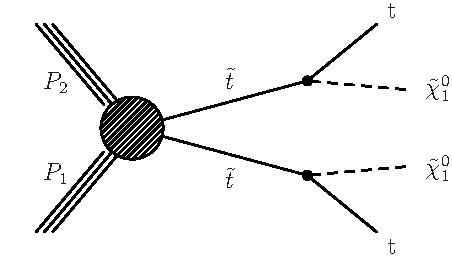
\includegraphics[width=0.40\textwidth]{sections/mc4/Introduction/figures/T2tt.pdf}\\
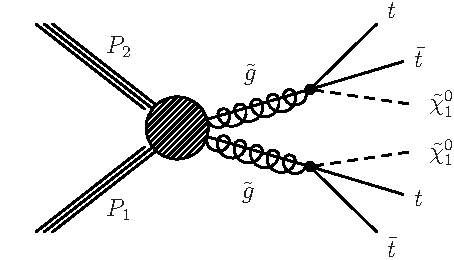
\includegraphics[width=0.33\textwidth]{sections/mc4/Introduction/figures/T1tttt_feynman.pdf}
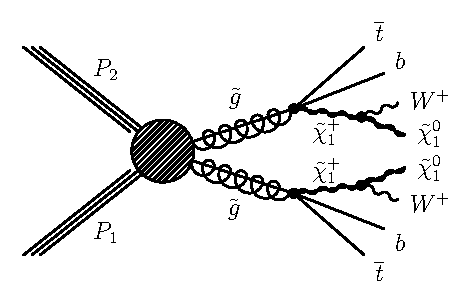
\includegraphics[width=0.33\textwidth]{sections/mc4/Introduction/figures/T1ttbb.pdf}\\
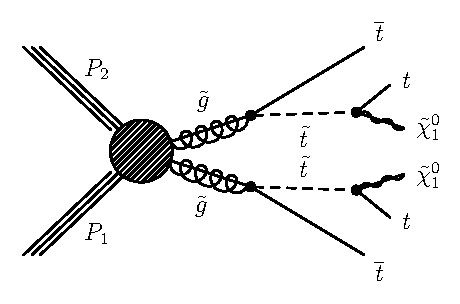
\includegraphics[width=0.33\textwidth]{sections/mc4/Introduction/figures/T5tttt.pdf}
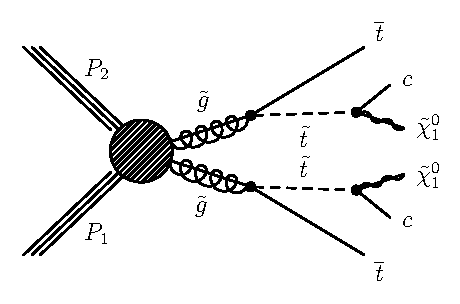
\includegraphics[width=0.33\textwidth]{sections/mc4/Introduction/figures/T5ttcc.pdf}\\
\caption{Signal models of interest in this search:
top squark pair production with the top squark decaying into a top quark and
neutralino (top),
and top squarks from cascade decays of gluinos (middle and bottom).
The SUSY simplified model topology shown at the top is referred to as T2tt,
the middle left model as T1tttt, middle right model as T1ttbb
the bottom left one as T5tttt and the bottom right one as T5ttcc.}
\label{fig:signal_diagrams}
\end{centering}
\end{figure}

The first step of the search is to design a search region with proper cuts. Since we are looking into all hadronic channels, we would veto the leptons and isolated tracks. The number of jets and \MET requirements are also needed to suppress the standard model background. A set of $\Delta\phi$ cuts between the \MET and several leading jets are also applied to reject QCD events. Moreover, since the signal final states have b-jets and top-jets, the numbers of b-jets and top-jets cuts are also added into the baseline selection. We use the official recommendation of b-jet tagger from CMS b-tagger working group. However, for the top-jet, we applied cut-based top jet identification in the 2015 analysis\cite{PhysRevD.96.012004}. In this 2016 analysis, we design a new top-jet identification algorithm to improve the analysis. Several working points are designed in top-jet tagger.

The next step is to determine the top-jet working point and optimize the search bins. We optimize the search bin definition for both medium and tight top-jet working point, and then choose the tight one because it is more sensitive for some signals.

Then, we need to estimate the backgrounds for all search bins. The major background is for TT-jets, W-jets and single top processes. The Z-jets, QCD, TTZ and other rare processes are not negligible, too.

Finally, we can set limit on the model parameters with the data yield, background estimation and targeting model yields. The interpretation is based on the simplified model\cite{Alwall:2008ag}.



\clearpage
\section{Customized top tagger}
\label{sec:c4tt}
\subsubsection{Motivation}
A cut-based top jet tagger is applied in 2015 paper for this analysis\cite{CMS-PAS-SUS-16-030}. The cut-based top jet tagger has a wonderful efficiency over the top pt spectrum. However, the mistag rate is also relatively high in this tagger. Therefore, we design a new top tagger to reduce the mistag rate. 

\subsubsection{Description of the method}

Before we move to the top tagger algorithm, let’s review the top decay modes. The top jet decay (Fig~\ref{fig:c4twdecaymod}) can be categorized into two classes: hadronically decayed tops and leptonically (and semi-leptonically) decayed tops. We focus on the hadronically decayed tops since we are searching SUSY in hadronic channels. The hadronically decayed tops can majorly be detected in three ways (Fig~\ref{fig:c4twdecaymod}): a fat mono-jet with mass close to top mass, a fat mono-jet with mass close to W mass and one b-jet, and 3 resolved jets. Our cut-based algorithm is designed following these three scenarios respectively. 

\begin{figure}[htbp]
 \begin{center}
  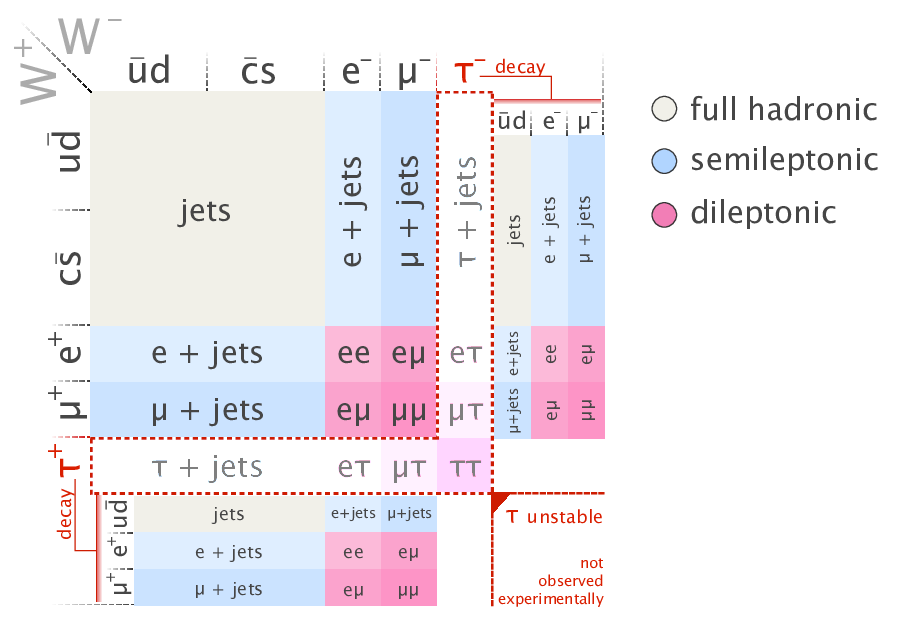
\includegraphics[width=0.55\textwidth]{figures/c4/c4_top_w_decaymod.png}
  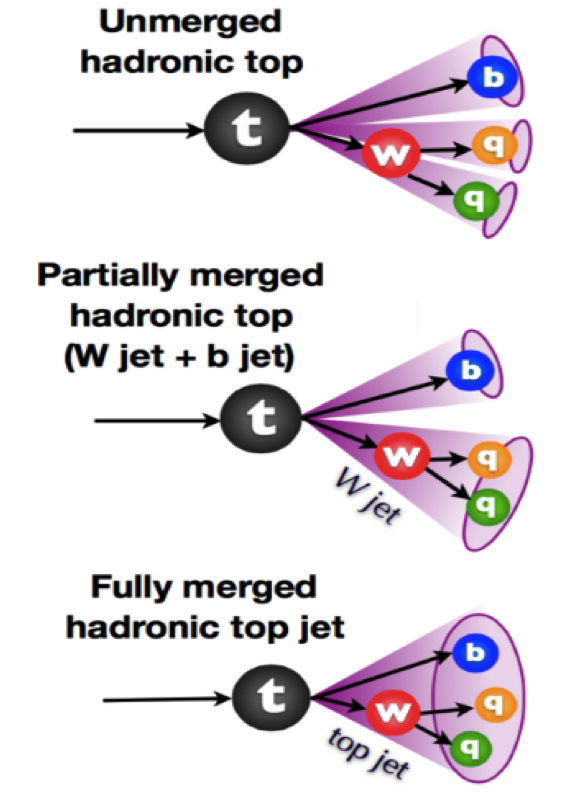
\includegraphics[width=0.25\textwidth]{figures/c4/c4_tagger_hadtopdecay.png}
 \end{center}
 \caption{Left: \ttbar events final states; Right: Hadronically decayed tops}
 \label{fig:c4twdecaymod}
\end{figure}

Only the small AK4 cone jet collection is used in the cut-based tagger to avoid jet removing from different collections. The side effect of this treatment is the remnant system can be relatively big in the mono-jet and di-jet case. The cut-based algorithm is not very powerful in the tri-jets system, compared with multi-variable algorithms. Therefore, the new top tagger has 2 major upgrades: fat jet (AK8 jet) for mono-jet and di-jet top decay, and multi-variable algorithm for tri-jet system. We expect lower mistag rate with the similar efficiencies after the upgrade. 

The mono-jet top selection is relatively simple. The requirements for the mono-AK8 jet are:
\begin{itemize}
\item AK8 jet $p_{T}\ge$400 GeV 
\item Soft drop mass between 105 and 210 GeV
\item N-subjettiness $\tau_{32}\le$0.65
\end{itemize}

If an AK8 jet is used in the mono-jet case, it will be removed from the jet collection for next steps. 

We require one W-like AK8 jet and b-like AK4 jet in the di-jet case. The W-like AK8 jet is selected with following requirements:
\begin{itemize}
\item AK8 jet $p_{T}\ge$200 GeV
\item Soft drop mass between 65 and 100 GeV
\item N-subjettiness $\tau_{21}\le$0.60
\end{itemize}

Then, the W-like AK8 jet will be combined with one AK4 jet with $p_{T}\ge$40 GeV. The additional requiremnets on the di-jet system is:
\begin{itemize}
\item di-jet system mass is between 100 to 250 GeV
\item di-jet system within R cone 1.0
\item jet mass ratio between AK8 W-like jet and di-jet system in range $[ 0.85 \frac{m_{W}}{m_{t}}, 1.25 \frac{m_{W}}{m_{t}} ]$
\end{itemize}

We start using both AK4 and AK8 jet collections from this step. We design an overlap remove algorithm to avoid jet energy reusing in the algorithm. A $\Delta R$ matching between AK4 jets and soft-drop sub-jets of the AK8 jets is applied for jet removal. 

As we mentioned before, multi-variable algorithm is applied to select the tri-jets top. There are two key elements in the multi-variable algorithm design: input variables and algorithm. 

In general, we have two input variables types: the high-level physics variables, like jet $p_{T}$, and base level physics variable, like particle flow candidate, and calorimeter pixels. The algorithm choosing is dependent on the input variables. For example, the high-level variables are more suited for the decision tree based algorithm, while base level variables prefer neutral network. 

We choose the high-level physics variables and decision tree based algorithm in our analysis. All three-jets combinations will be the potential top candidates. The following variables are considered in the algorithm: 
\begin{itemize}
\item Top candidate properties: mass, $p_{T}$, R cone size;
\item Constituent jet properties: jet $p_{T}$, $\eta$, $\phi$; CSV value (b-tag likelyhood), quark-gluon discriminator;
\item Angular variables between jets: $\Delta \phi, \Delta \eta, \Delta R$
\end{itemize}
%todo add QGL

All the variables are carefully studied before we put them into training. Let’s use quark gluon discriminator as an example. The quark gluon discriminator is likelihood to separate the quark jet and gluon jet. The value of the likelihood close to 1 means it is more like a quark jet, otherwise a gluon jet. The likelihood is constructed from three variables: 
\begin{itemize}
\item $p_{T}$D: jet energy dispersion variable, defined as $ $, with sum over all PF candidates
\item Mutiplicity: the total number of particle flow candidates that reconstructed within the jet
\item Axis2: minor axis RMS in the $\eta - \phi$ plane of the particle flow candidates
\end{itemize}

The multi-variable algorithm is better in digging out the correlation between training variables. The algorithm with the clean input variables can obtain the correlation features. Therefore, we need to study the performance of quark gluon discriminator on different jet flavors, $p_{T}$ and $\eta$. We studied the following jet flavors in the ttbar simulation samples: light flavor jet, c-jet, b-jet, gluon jet and pile-up jet. The $p_{T}$ and $\eta$ schemes are listed in the Table~\ref{tab:c4ttqgl}.

\begin{table}[htbp]
\fontsize{10 pt}{1.2 em}
\selectfont
\begin{centering}
\caption{\label{tab:c4ttqgl} Jet bin for quark-gluon discriminator study}
\hspace*{-4ex}
\begin{tabular}{|c|c|c|c|c|c|c|}
\hline
Jet $\eta$ Bin  & 1(HB) & 2(HBHE) & 3(HE) & 4(HEHF) & 5(HF) & 6(HF,no PDF) \\
\hline
Jet $\eta$      & [0,1.305] & [1.305,1.392] & [1.392,2.650] & [2.650,3.139] & [3.139,4.7] & [4.7,5.191] \\
\hline
Jet $p_{T}$ Bin & 1(no PDF) & 2 & 3 & 4 & 5 & 6 \\
\hline
Jet $p_{T}$     & [0,20] & [20,40] & [40,50] & [50,80] & [80,100] & [100,Inf] \\
\hline
\end{tabular}
\par\end{centering}
\end{table}

The performance in terms of jet $\eta$ in different jet flavors is showed in Fig~\ref{fig:c4ttqgljeteta}. The discrimination power for low $p_{T}$ jets is not ideal. 
\begin{figure}[htbp]
 \begin{center}
  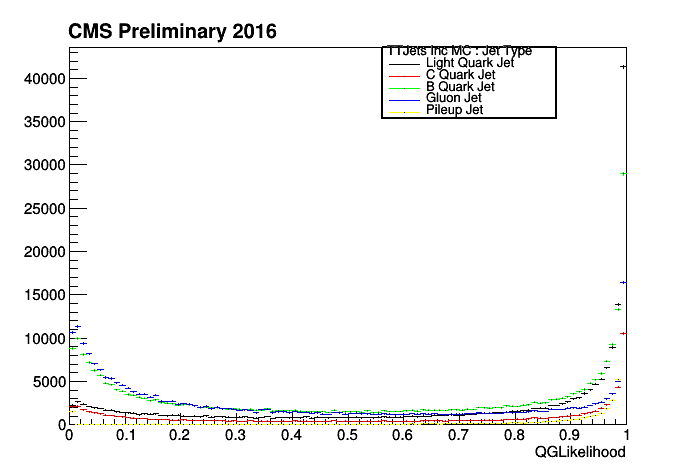
\includegraphics[width=0.45\textwidth]{sections/mc4/TopTagger/figures/_b_qglikelihoodjetetabin0_.png}
  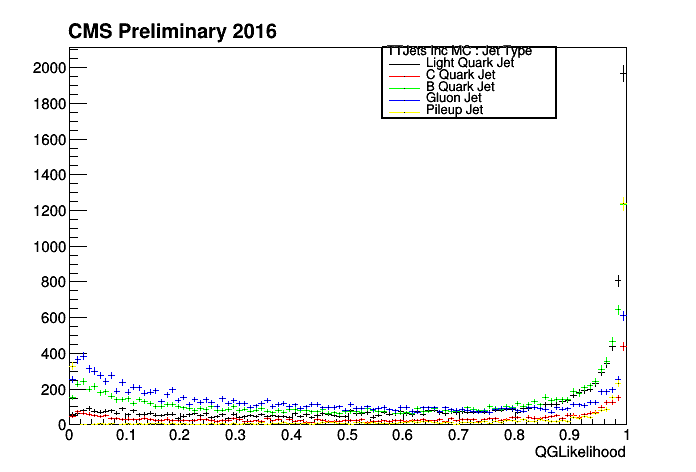
\includegraphics[width=0.45\textwidth]{sections/mc4/TopTagger/figures/_b_qglikelihoodjetetabin1_.png} \\
  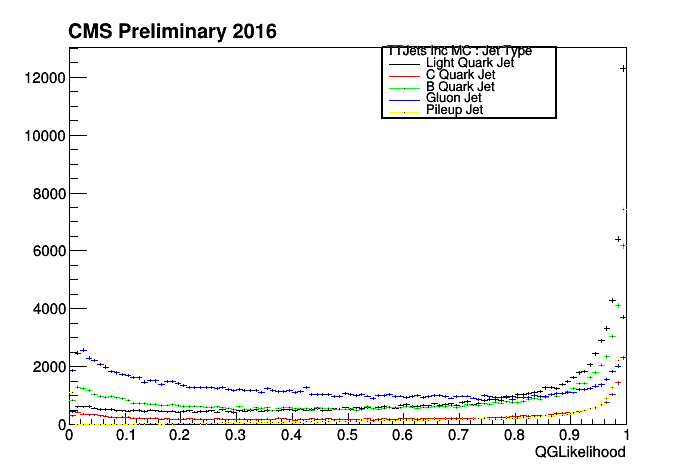
\includegraphics[width=0.45\textwidth]{sections/mc4/TopTagger/figures/_b_qglikelihoodjetetabin2_.png}
  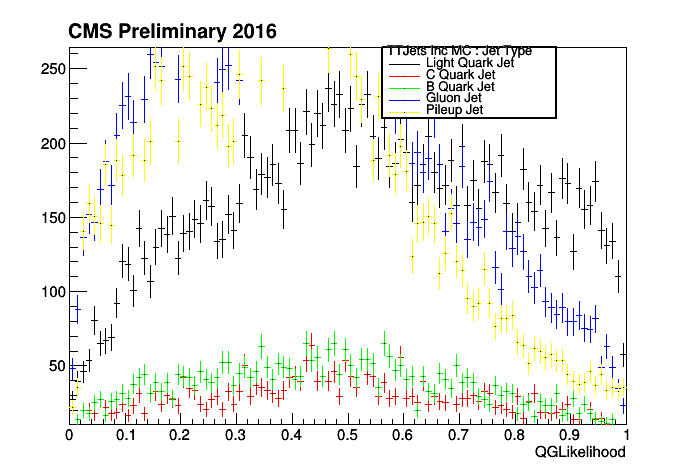
\includegraphics[width=0.45\textwidth]{sections/mc4/TopTagger/figures/_b_qglikelihoodjetetabin3_.png} \\
  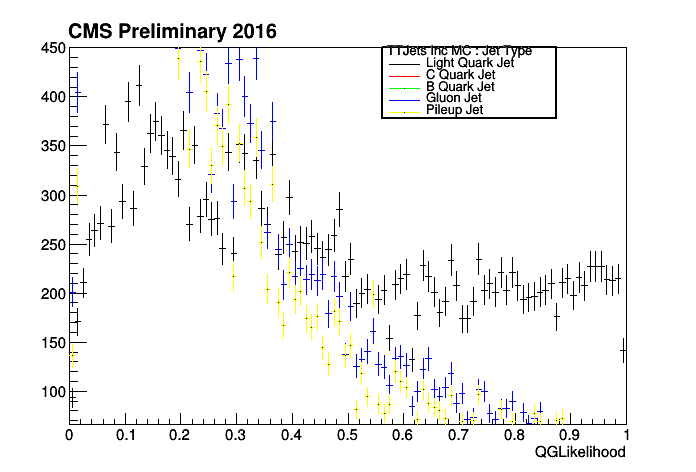
\includegraphics[width=0.45\textwidth]{sections/mc4/TopTagger/figures/_b_qglikelihoodjetetabin4_.png}
  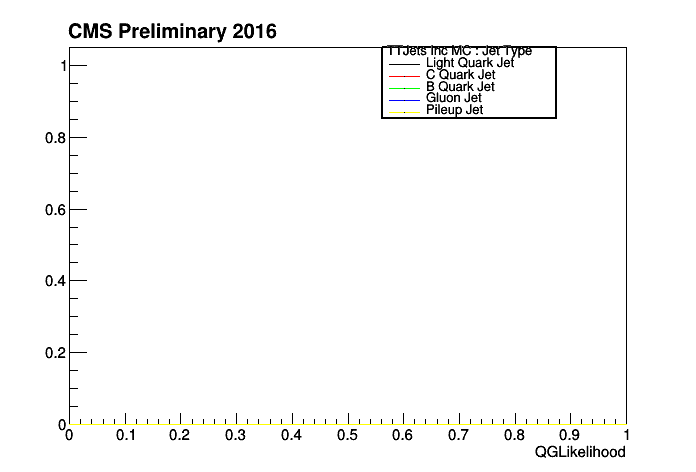
\includegraphics[width=0.45\textwidth]{sections/mc4/TopTagger/figures/_b_qglikelihoodjetetabin5_.png}
 \end{center}
 \caption{Top left: Quark Gluon likelihood for jet $\eta$ bin 1; Top right: jet $\eta$ bin 2; Middle left: jet $\eta$ bin 3; Middle right: jet $\eta$ bin 4; Middle left: jet $\eta$ bin 5; Middle right: jet $\eta$ bin 6}
 \label{fig:c4ttqgljeteta}
\end{figure}

The performance in terms of jet $p_{T}$ in different jet flavors is showed in Fig~\ref{fig:c4ttqgljetpt}. The discrimination power for HEHF and HF jets is not ideal.
\begin{figure}[htbp]
 \begin{center}
  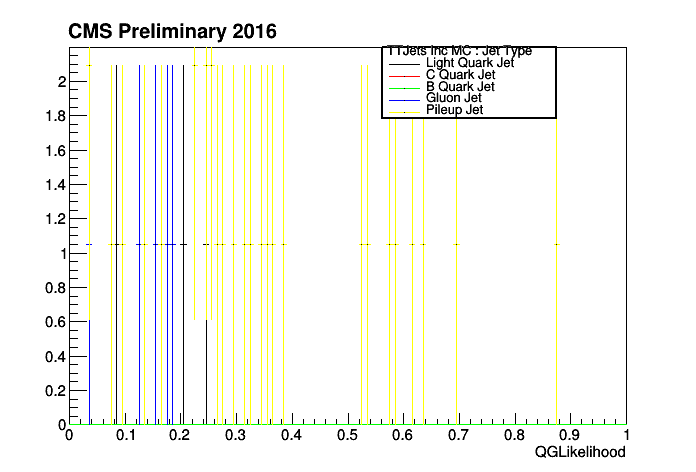
\includegraphics[width=0.45\textwidth]{sections/mc4/TopTagger/figures/_b_qglikelihoodjetptbin0_.png}
  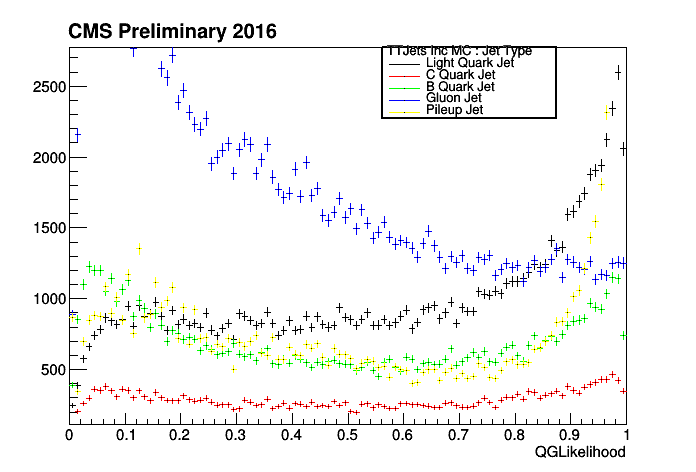
\includegraphics[width=0.45\textwidth]{sections/mc4/TopTagger/figures/_b_qglikelihoodjetptbin1_.png} \\
  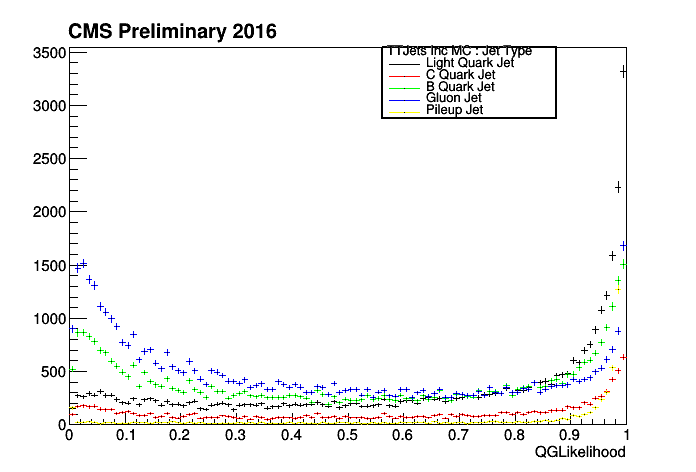
\includegraphics[width=0.45\textwidth]{sections/mc4/TopTagger/figures/_b_qglikelihoodjetptbin2_.png} 
  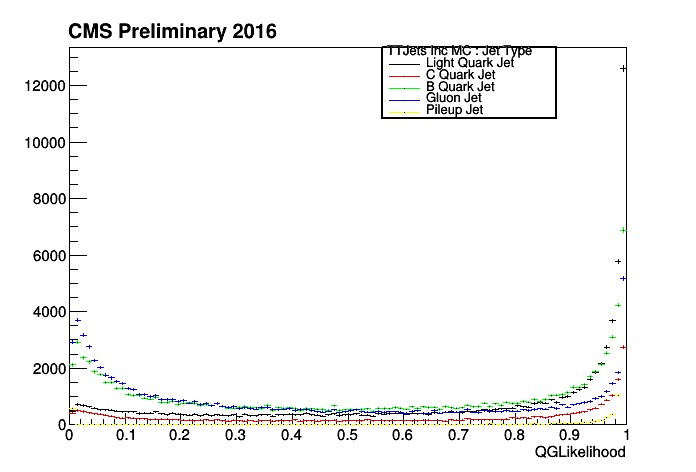
\includegraphics[width=0.45\textwidth]{sections/mc4/TopTagger/figures/_b_qglikelihoodjetptbin3_.png} \\
  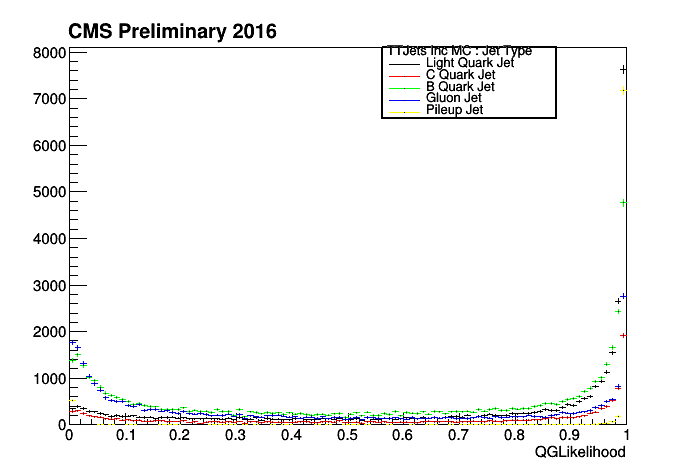
\includegraphics[width=0.45\textwidth]{sections/mc4/TopTagger/figures/_b_qglikelihoodjetptbin4_.png}
  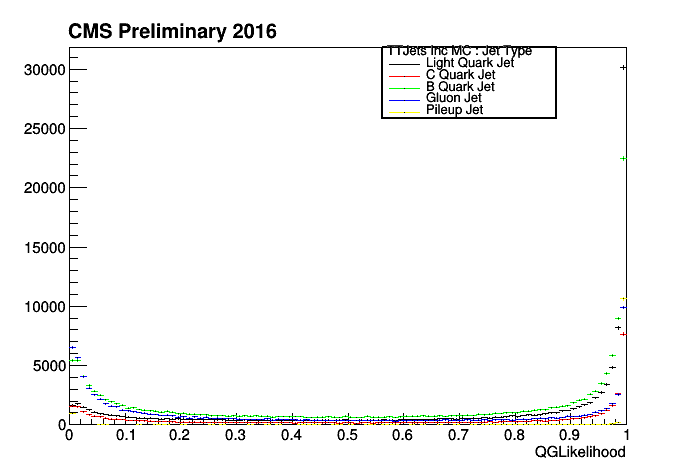
\includegraphics[width=0.45\textwidth]{sections/mc4/TopTagger/figures/_b_qglikelihoodjetptbin5_.png}
 \end{center}
 \caption{Top left: Quark Gluon likelihood for jet $p_{T}$ bin 1; Top right: jet $p_{T}$ bin 2; Middle left: jet $p_{T}$ bin 3; Middle right: jet $p_{T}$ bin 4; Middle left: jet $p_{T}$ bin 5; Middle right: jet $p_{T}$ bin 6}
 \label{fig:c4ttqgljetpt}
\end{figure}

And, the quark gluon discriminator is now working well with b-jet for all cases. Therefore, we decide to force the likelihood to be 1 (quark jet) in case of a tagged b-jet before training. 

All the variables are feed into random forest\cite{Ho:1995:RDF:844379.844681} training algorithm for training in simulation samples. The final top-jet efficiencies are about 0.6. The mistag rate about 0.2, 50\% reduced compared with the cut-based legacy tagger. Now, we complete our tagging algorithm in full simulation samples. We still need to study the difference between the full simulation and data, and also full simulation and fast simulation, since we are using fast simulation signals for limit setting. The scale factors are binned in the top-jet $p_{T}$ and applied in the data card before limit setting. More details are demonstrated in\cite{AN-16-461}. 


\clearpage
\section{Event selection and search bin design}
\label{sec:c4evssbd}
As we mentioned at the begining of chapter 4, The analysis is designed for maximum sensitivity to the SUSY simplified model T2tt, T1tttt, T1ttbb, T5tttt and T5ttcc topology resulting in final states with multiple top quarks, hence multiple jets and b-tagged jets, produced in stop decay, no leptons, and large \MET. The T2tt, T5ttcc and T1tttt final states differ in the number of jets, b-tagged jets and top quarks produced. 

Targeting the above-mentioned final states, data are initially selected by requiring a number of jets and b-jets (\njets and \nbjets) and a large \MET. The search regions are ultimately defined in exclusive bins of \ntops, \nbjets, \HT, \MET and \MTTwo. SM backgrounds come from processes such as \ttbar QCD multijet events, Z+jets, W/top+jets, and smaller contributions from rare processes.

The data selection process starts with the triggers and follows with a pre-selection and the definition of the search bins. The top reconstruction and identification procedure (top tagging) is described in this section, as well as the Monte Carlo (MC) samples that model signal and backgrounds.

\subsection{Trigger}
\label{sec:trig}
Six search triggers are used to collect events for this analysis. They are seeded by \MET seed in Level-1 trigger. 
\begin{itemize}
\item \texttt{ HLT\_PFMET100\_PFMHT100\_IDTight\_v*}
\item \texttt{ HLT\_PFMET110\_PFMHT110\_IDTight\_v*}
\item \texttt{ HLT\_PFMET120\_PFMHT120\_IDTight\_v*}
\item \texttt{ HLT\_PFMETNoMu100\_PFMHTNoMu100\_IDTight\_v*} 
\item \texttt{ HLT\_PFMETNoMu110\_PFMHTNoMu110\_IDTight\_v* }
\item \texttt{ HLT\_PFMETNoMu120\_PFMHTNoMu120\_IDTight\_v*}
\end{itemize}

The probability for these triggers to accept events (trigger efficiency) is
measured in a sample of events collected by the single-electron trigger
\begin{itemize}
  \item \texttt{HLT\_Ele27\_WPTight\_v*},
\end{itemize}
which has been commonly used within CMS for the \MET trigger efficiency measurement. 
Event from the single electron dataset is required to have
\texttt{HLT\_Ele27\_WPTright\_v*} trigger, also has at least one offline
reconstructed electron with $p_{T}>$ 30GeV. These selections ensure the single
electron trigger is efficient. 

To measure the search trigger efficiency, additional cuts to mimic the
pre-selection, defined in Sec.~\ref{sec:pre-selection}, are required.
\begin{itemize}
  \item Pass all filters
  \item Veto reconstructed muon
  \item $\njets\geq4$
  \item \nbjets $\ge$ 1
  \item \HT $\ge$ 300 GeV
  \item $\Delta\phi(\MET, j_{1,2,3})>$ 0.5, 0.5, 0.3
\end{itemize}

The trigger efficiency of the search triggers is measured as a function of
the offline \MET.  The events passed the above requirements are defined as the
denominator, while the above events also triggered the search triggers are
defined as the numerator. It has been found that the \MET trigger efficiency
has a non-trivial dependency on the offline $\HT$. The search trigger
efficiencies are measured in the low $\HT$ (300 $< \HT <$ 1000) and high
$\HT$ ($\HT >$ 1000) region, as shown in Fig.~\ref{fig:TrigMET}.
\begin{figure}[tbp]
 \begin{center}
   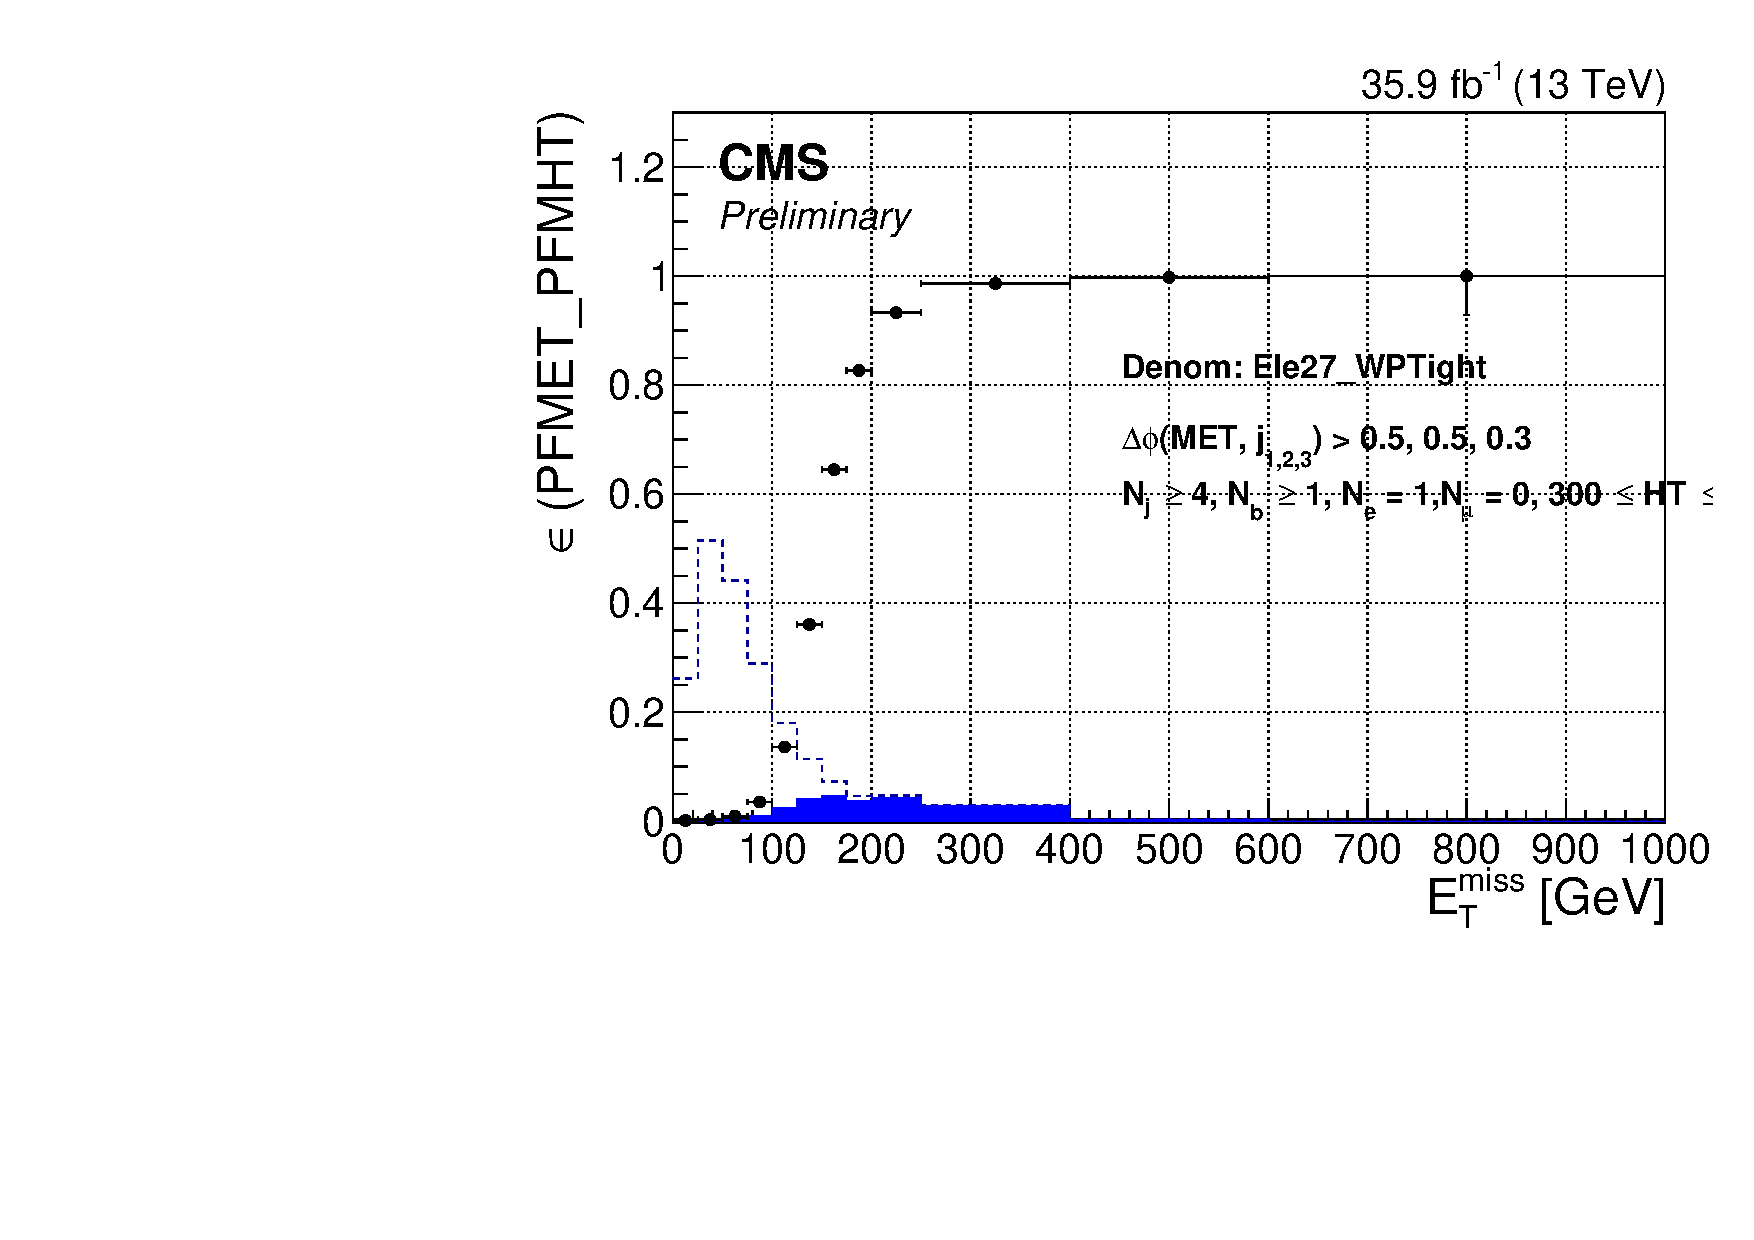
\includegraphics[width=0.49\linewidth]{sections/mc4/EvtSelSBOpt/figures/TrigEle_Stop_TrigMET_HTLess1000_9.pdf}
   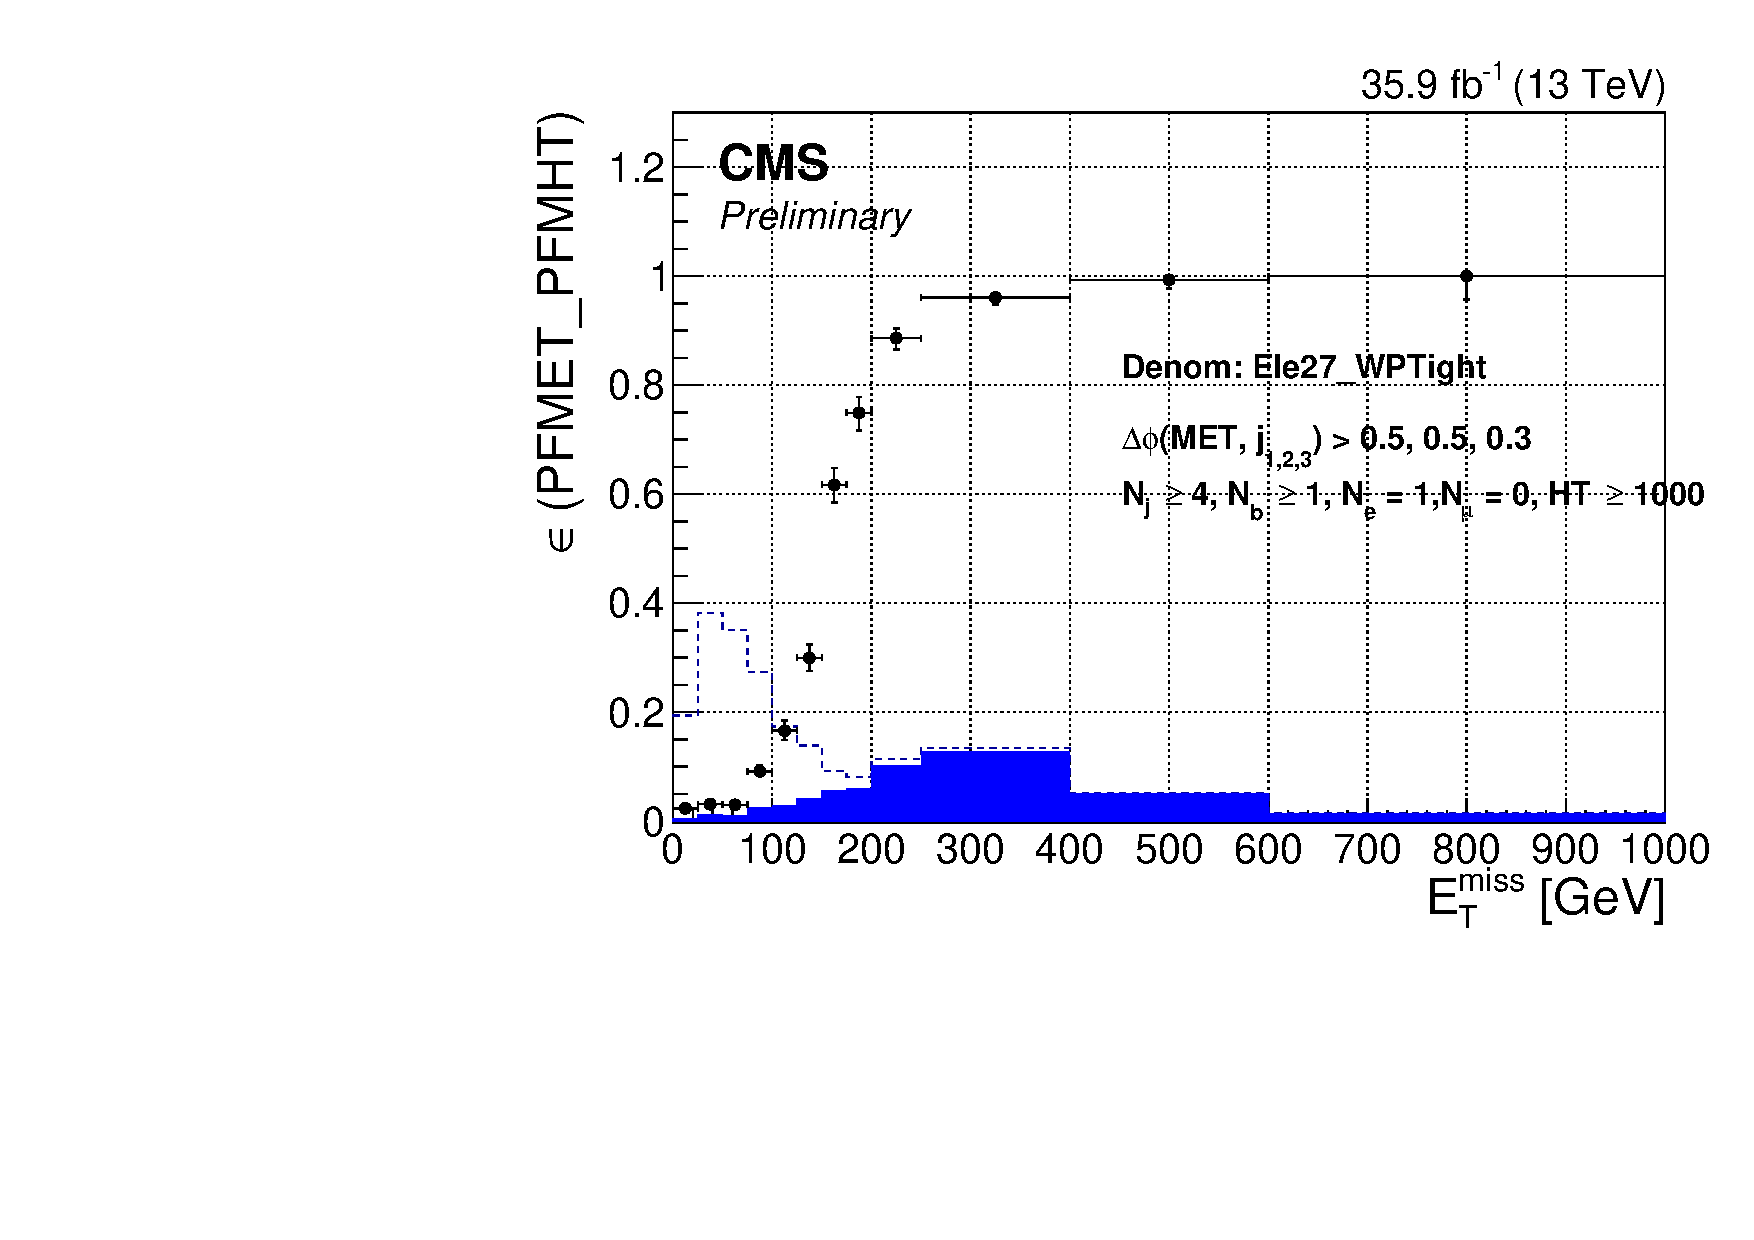
\includegraphics[width=0.49\linewidth]{sections/mc4/EvtSelSBOpt/figures/TrigEle_Stop_TrigMET_HTMore1000_9.pdf}
   \caption{ The trigger efficiency, denote by the black point, as a function
   of the offline \MET for (left) 300 $< \HT <$ 1000 and (right) $\HT >$ 1000.
   The error bar indicates the statistical uncertainty of the trigger
   efficiency. The dash blue line represents the denominator passing the
   selection, while the solid blue histogram represents the numerator where
   the denominator events also trigger the search triggers. }
   \label{fig:TrigMET}
 \end{center}
\end{figure}

Beside measuring the \MET trigger efficiency from the single electron dataset,
the same trigger efficiency can be measured from single muon and HTMHT
dataset. To account for possible bias from different measurements, we will
take the measurement from the single-electron dataset as the nominal and the
variation from the measurements from single-muon and HTMHT dataset as
systematic uncertainty of the trigger efficiency, as shown in
Fig.~\ref{fig:TrigMETSys}. For \MET above 250GeV, we observe similar \MET
trigger efficiency, with systematic uncertainty less than 1\%.

For \MET trigger efficiency measured from single-muon dataset, events are collected by the single-muon trigger
\begin{itemize}
  \item \texttt{HLT\_Mu50\_v*},
\end{itemize}
with requrements below:
\begin{itemize}
  \item Pass all filters
	\item Leading reconstructed muon with $p_{T}>$ 50GeV
  \item Veto reconstructed electron
  \item $\njets\geq4$
  \item \nbjets $\ge$ 1
  \item \HT $\ge$ 300 GeV
  \item $\Delta\phi(\MET, j_{1,2,3})>$ 0.5, 0.5, 0.3
\end{itemize}
For \MET trigger efficiency measured from HTMHT dataset, events are
collected by the HT triggers
\begin{itemize}
  \item \texttt{HLT\_PFHT200\_v*},
  \item \texttt{HLT\_PFHT250\_v*},
  \item \texttt{HLT\_PFHT300\_v*},
  \item \texttt{HLT\_PFHT350\_v*},
  \item \texttt{HLT\_PFHT400\_v*},
  \item \texttt{HLT\_PFHT475\_v*},
  \item \texttt{HLT\_PFHT600\_v*},
  \item \texttt{HLT\_PFHT800\_v*},
  \item \texttt{HLT\_PFHT900\_v*},
  \item \texttt{HLT\_CaloJet500\_NoJetID\_v*},
\end{itemize}, 
in which \texttt{HLT\_CaloJet500\_NoJetID\_v*} is recommended by Level-1 for
recovering the inefficiency of L1\_HTT trigger during period H data taking.
Event are required to pass below selections:
\begin{itemize}
  \item Pass all filters
  \item Veto reconstructed electron
  \item Veto reconstructed muon
  \item $\njets\geq4$
  \item \nbjets $\ge$ 1
  \item \HT $\ge$ 300 GeV
  \item $\Delta\phi(\MET, j_{1,2,3})>$ 0.5, 0.5, 0.3
\end{itemize}

\begin{figure}[tbp]
 \begin{center}
   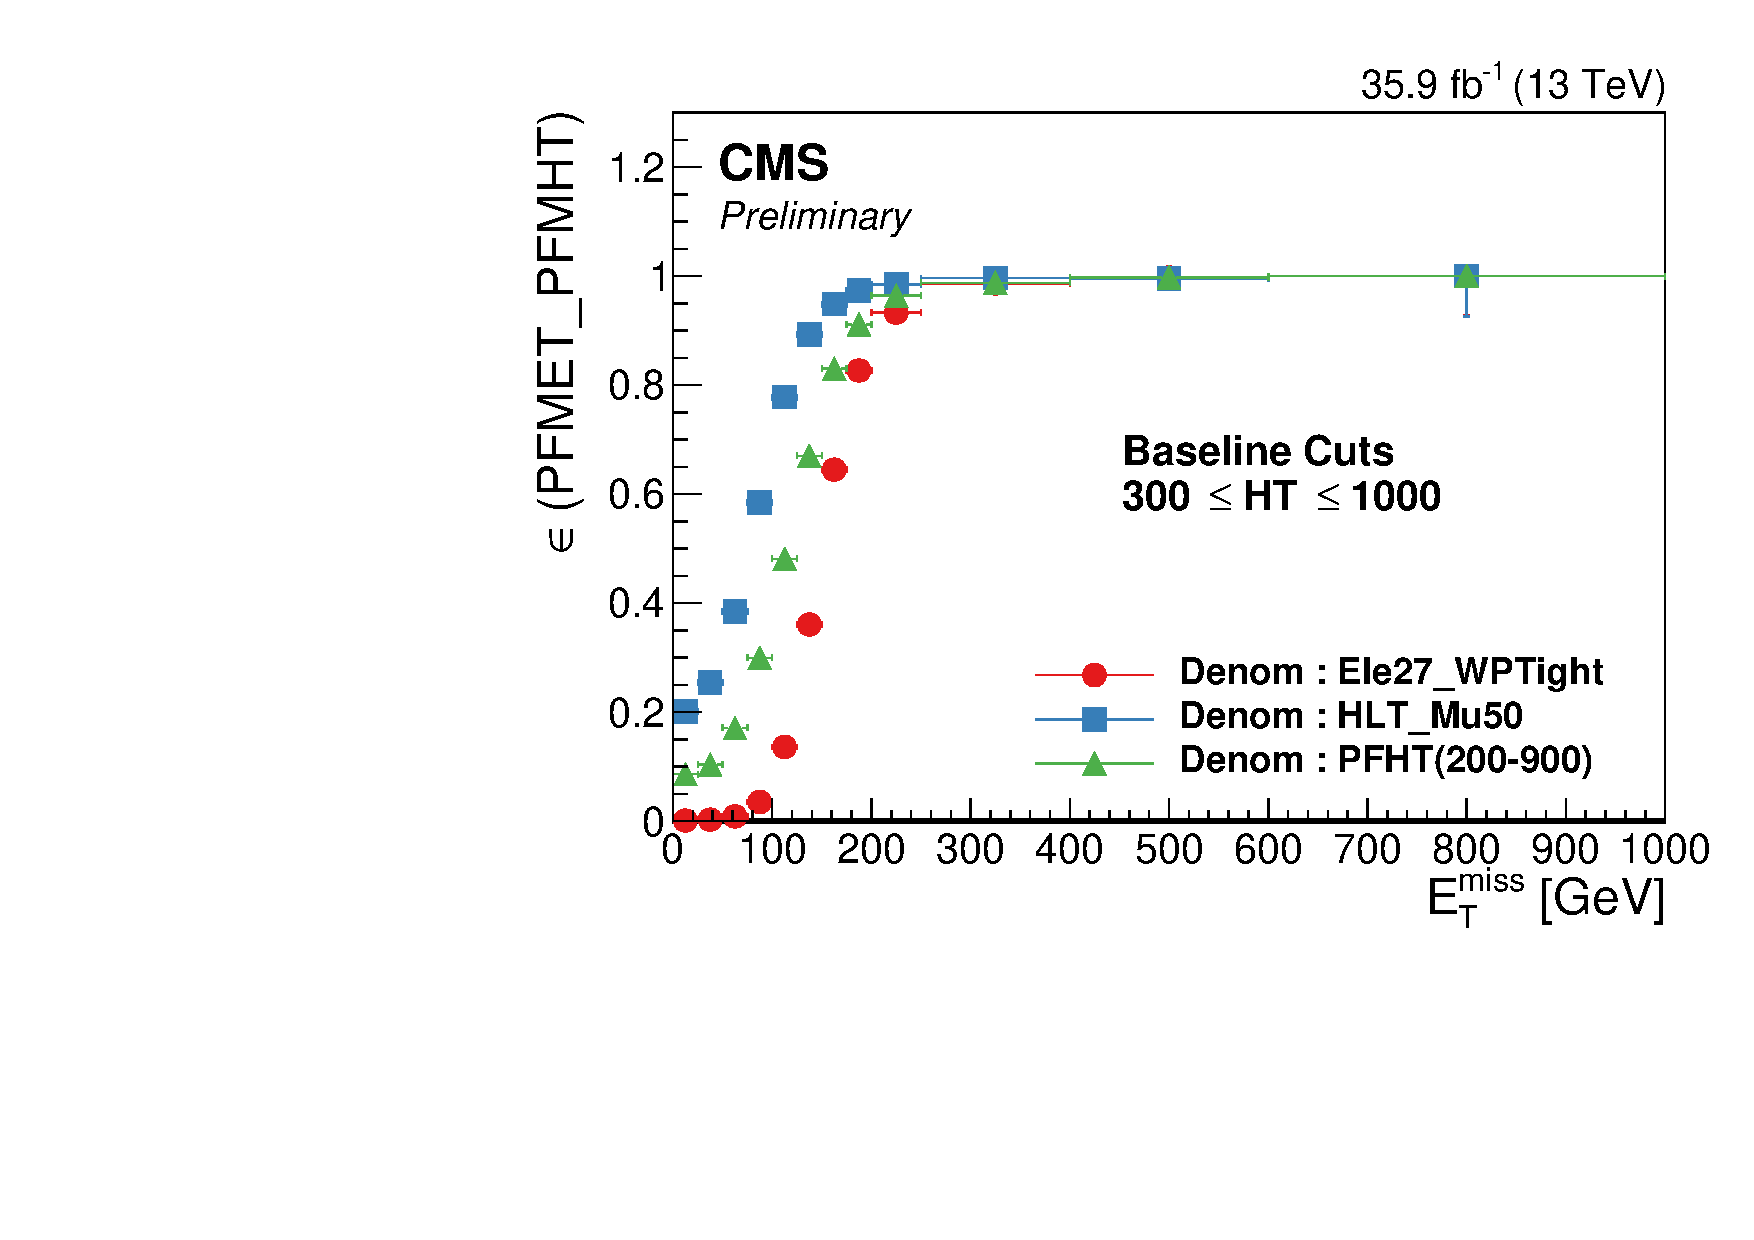
\includegraphics[width=0.49\linewidth]{sections/mc4/EvtSelSBOpt/figures/TrigMET_HTLess1000.pdf}
   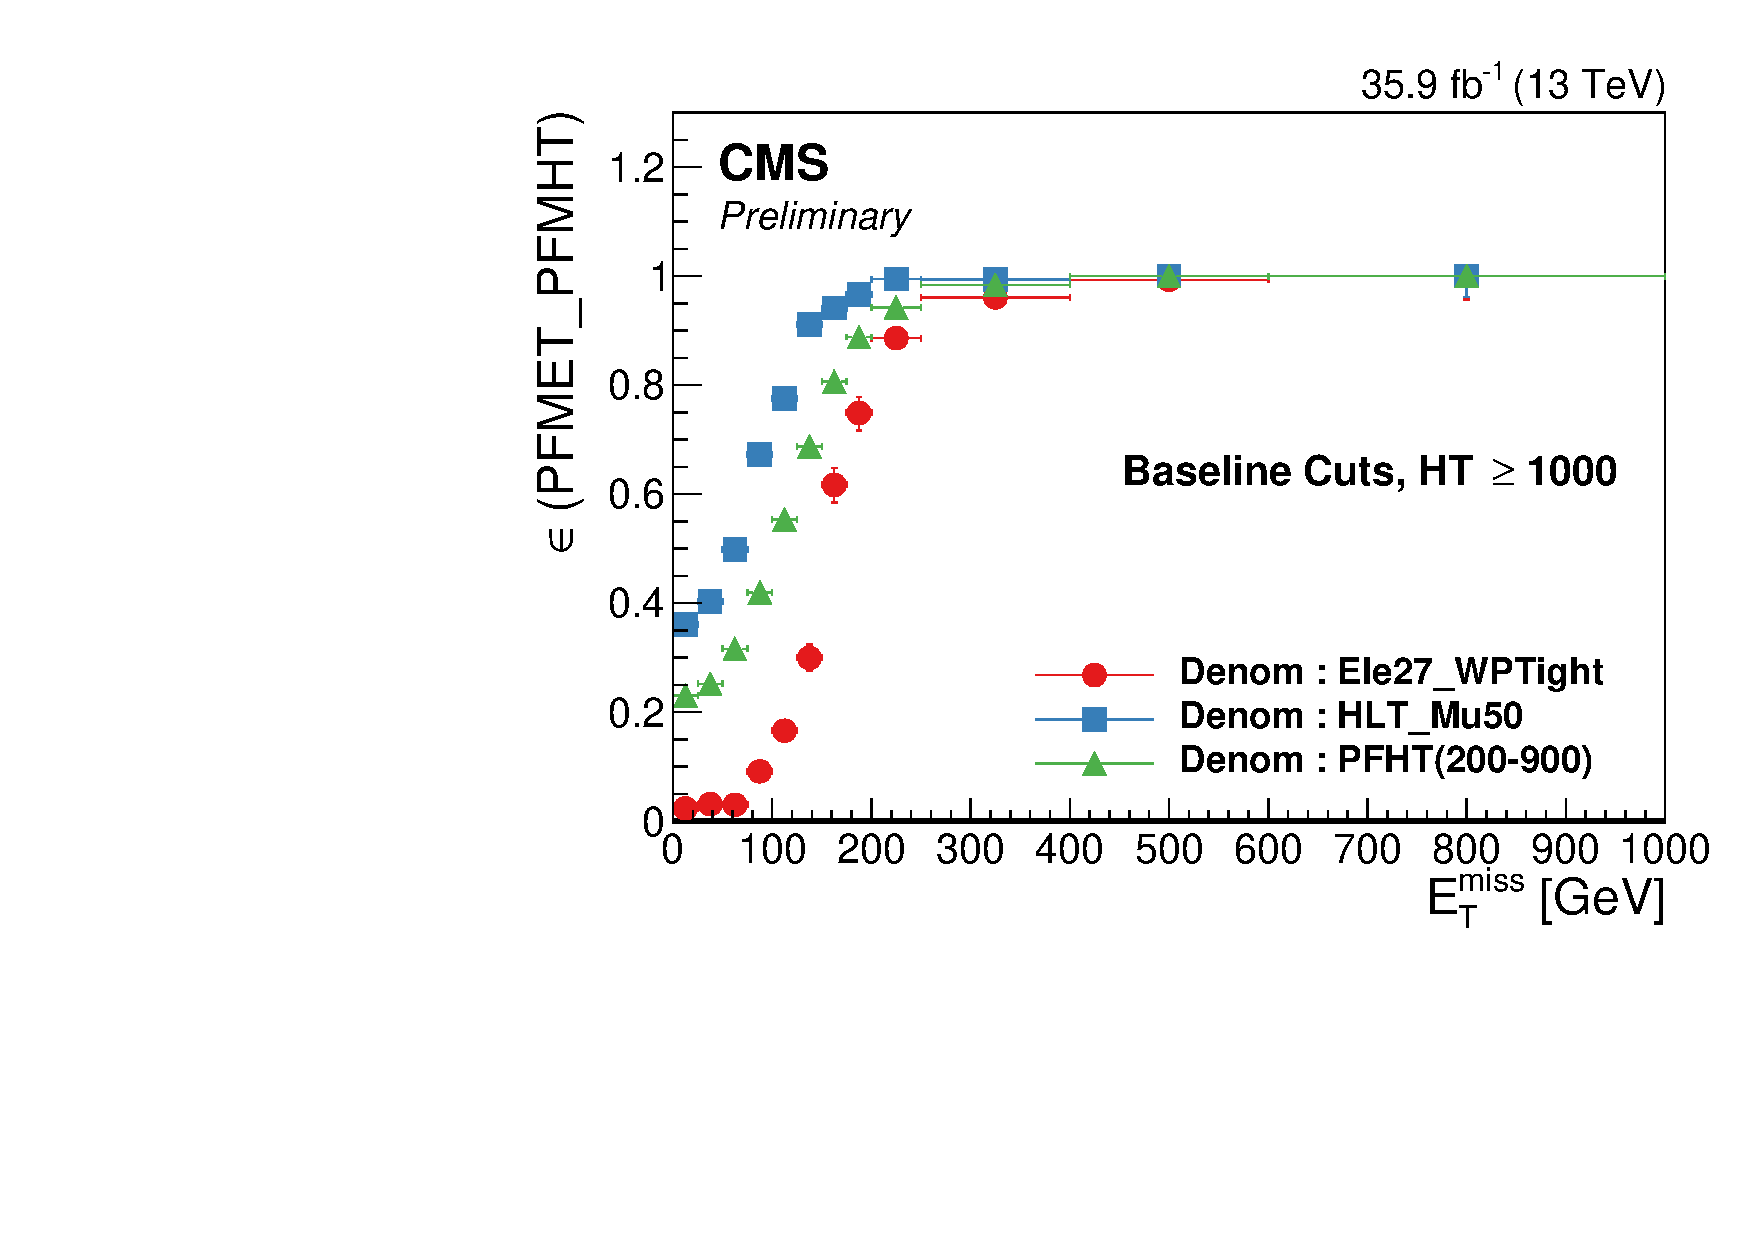
\includegraphics[width=0.49\linewidth]{sections/mc4/EvtSelSBOpt/figures/TrigMET_HTMore1000.pdf}
   \caption{ The trigger efficiency, denote by the black point, as a function
   of the offline \MET for (left) 300 $< \HT <$ 1000 and (right) $\HT >$ 1000.
   The error bar indicates the statistical uncertainty of the trigger
   efficiency. The blue square represents efficiency measured with
   single-muon dataset.  The red point represents efficiency measured
   with single-electron dataset while the green triangle represents
   efficiency measured with HT dataset.}
   \label{fig:TrigMETSys}
 \end{center}
\end{figure}

We also checked the trigger efficiency as a function of number of AK4 jets and
$b$-tagged jets, after requiring \MET $>$ 250GeV, as shown in
Fig.~\ref{fig:TrigMETJets}. Similar efficiencies are observed from different
measurements.

\begin{figure}[tbp]
 \begin{center}
   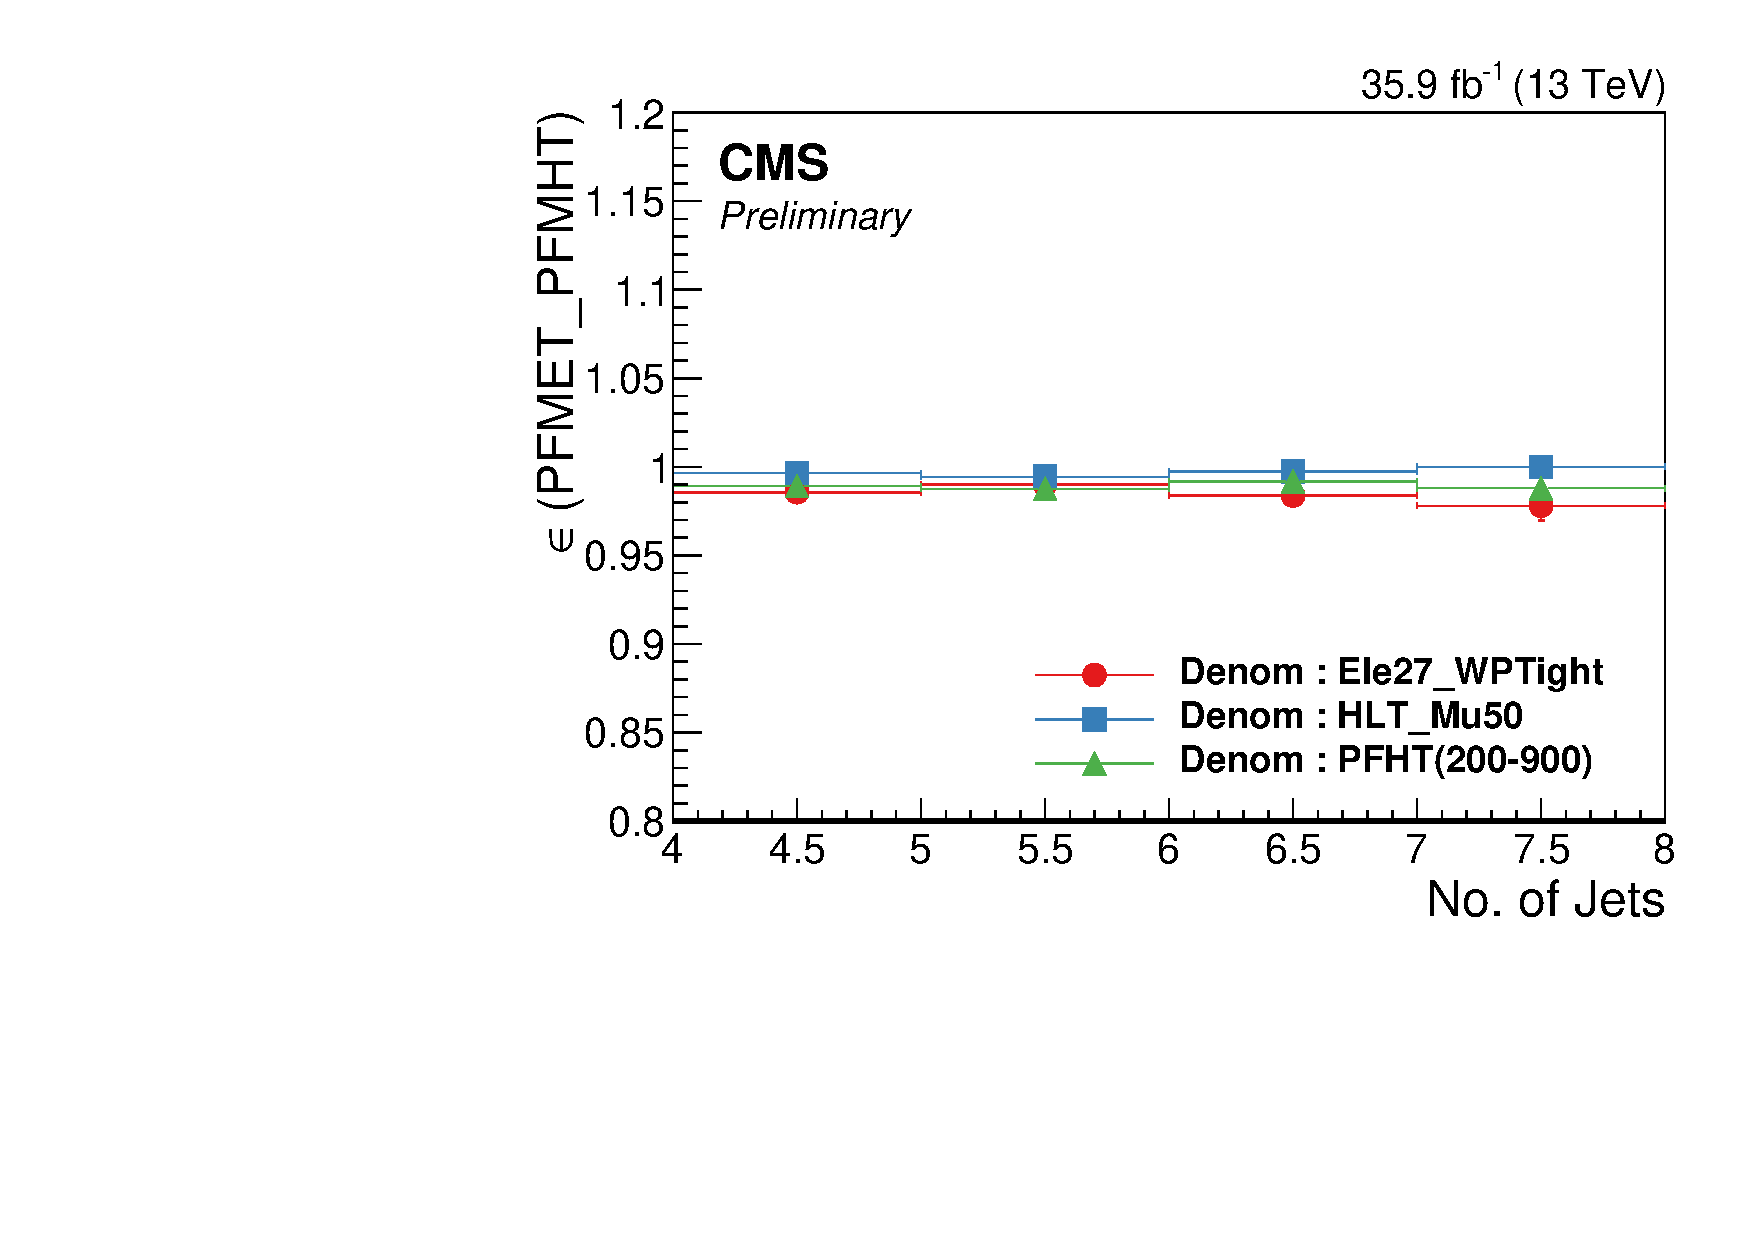
\includegraphics[width=0.49\linewidth]{sections/mc4/EvtSelSBOpt/figures/TrigNJets.pdf}
   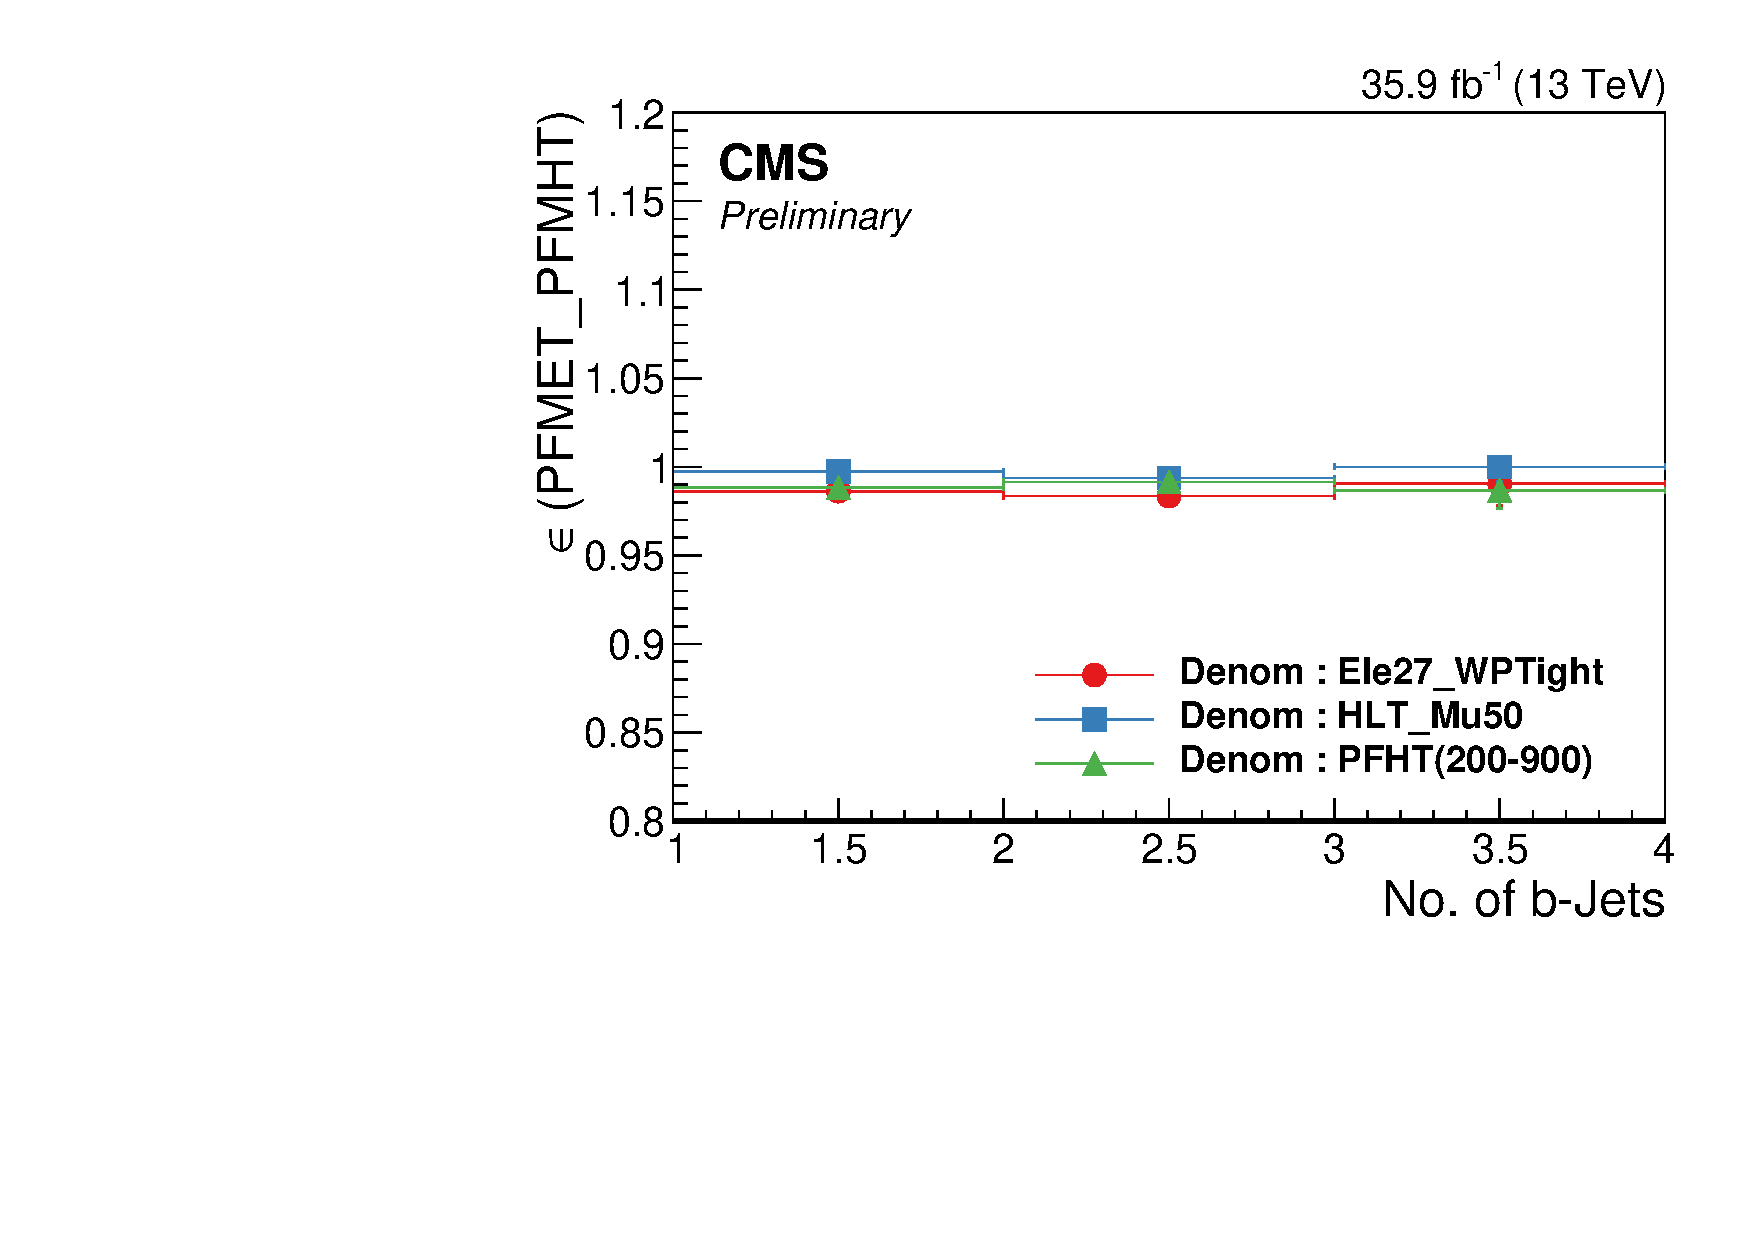
\includegraphics[width=0.49\linewidth]{sections/mc4/EvtSelSBOpt/figures/TrigNBs.pdf}
   \caption{ The trigger efficiency, denote by the black point, as a function
		 of the offline (left) number of jets with $p_{T}>$ 30 GeV and (right) number
		 of $b$-tagged jets with $p_{T}>$ 30GeV. The error bar indicates the
   statistical uncertainty of the trigger efficiency. The blue square
   represents efficiency measured with single-muon dataset.  The red point
   represents efficiency measured with single-electron dataset while the green
   triangle represents efficiency measured with HT dataset.}
   \label{fig:TrigMETJets}
 \end{center}
\end{figure}

The QCD background are estimated using the events triggered by search
triggers, but with cuts to select the QCD-enriched region. Since there are no
real \MET in QCD sample, the \MET trigger efficiency in the QCD-enriched
region would be different from the search region in the low \MET region. A
measurement of the trigger efficiency in the QCD-enriched region is carried
out in the HTMHT dataset to avoid bias. Events are required to pass the
similar cuts as the search trigger efficiency measurement, except an inverted
$\Delta\phi(\MET, j_{1,2,3})$ requirement as blow:
\begin{itemize}
  \item Pass all filters
  \item Veto reconstructed electron
  \item Veto reconstructed muon
  \item $\njets\geq4$
  \item \nbjets $\ge$ 1
  \item \HT $\ge$ 300 GeV
  \item $\Delta\phi(\MET, j_{1,2,3})<$ 0.5, 0.5, 0.3
\end{itemize}
The trigger efficiency is measured as a function of the offline \MET and showed in Fig.~\ref{fig:TrigMETQCD}.
\begin{figure}[tbp]
 \begin{center}
   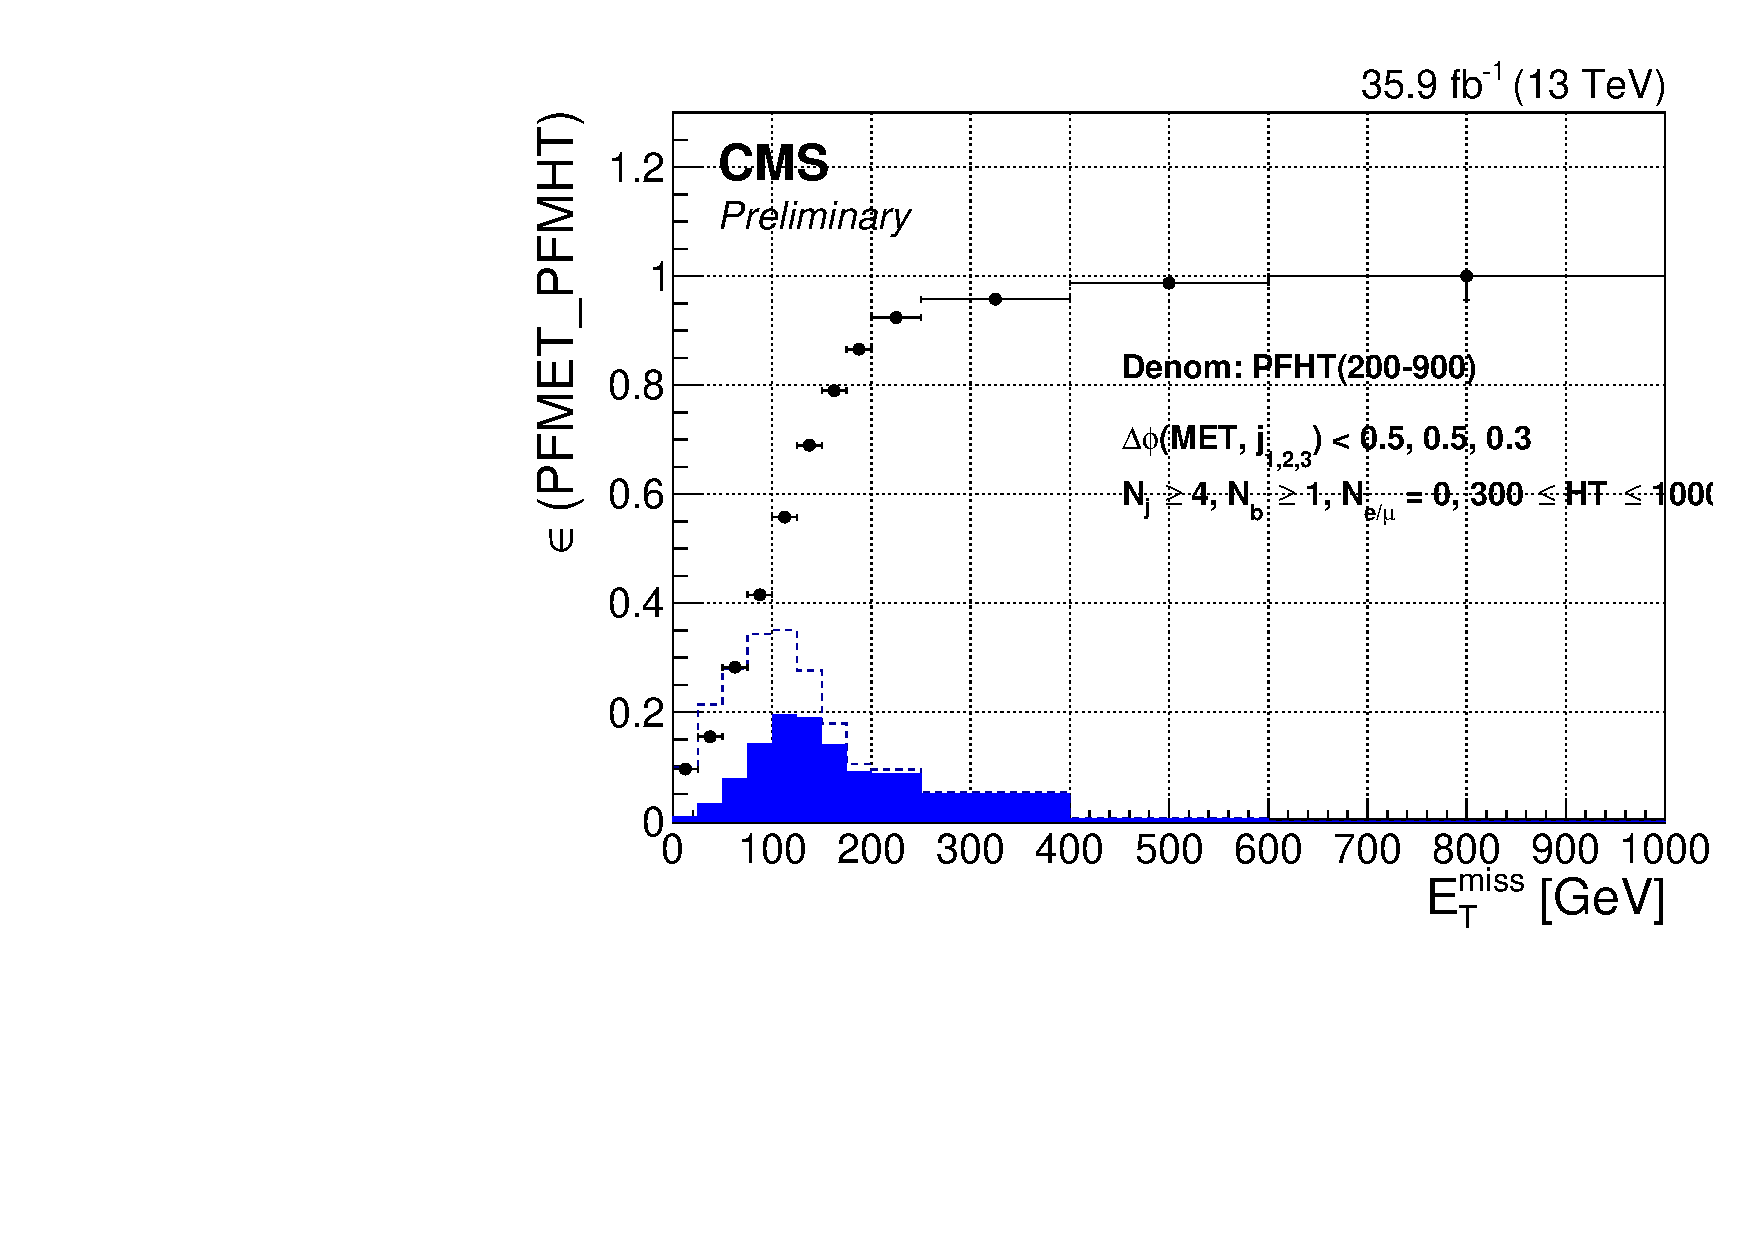
\includegraphics[width=0.49\linewidth]{sections/mc4/EvtSelSBOpt/figures/TrigHT_QCD_TrigMET_HTLess1000_9.pdf}
   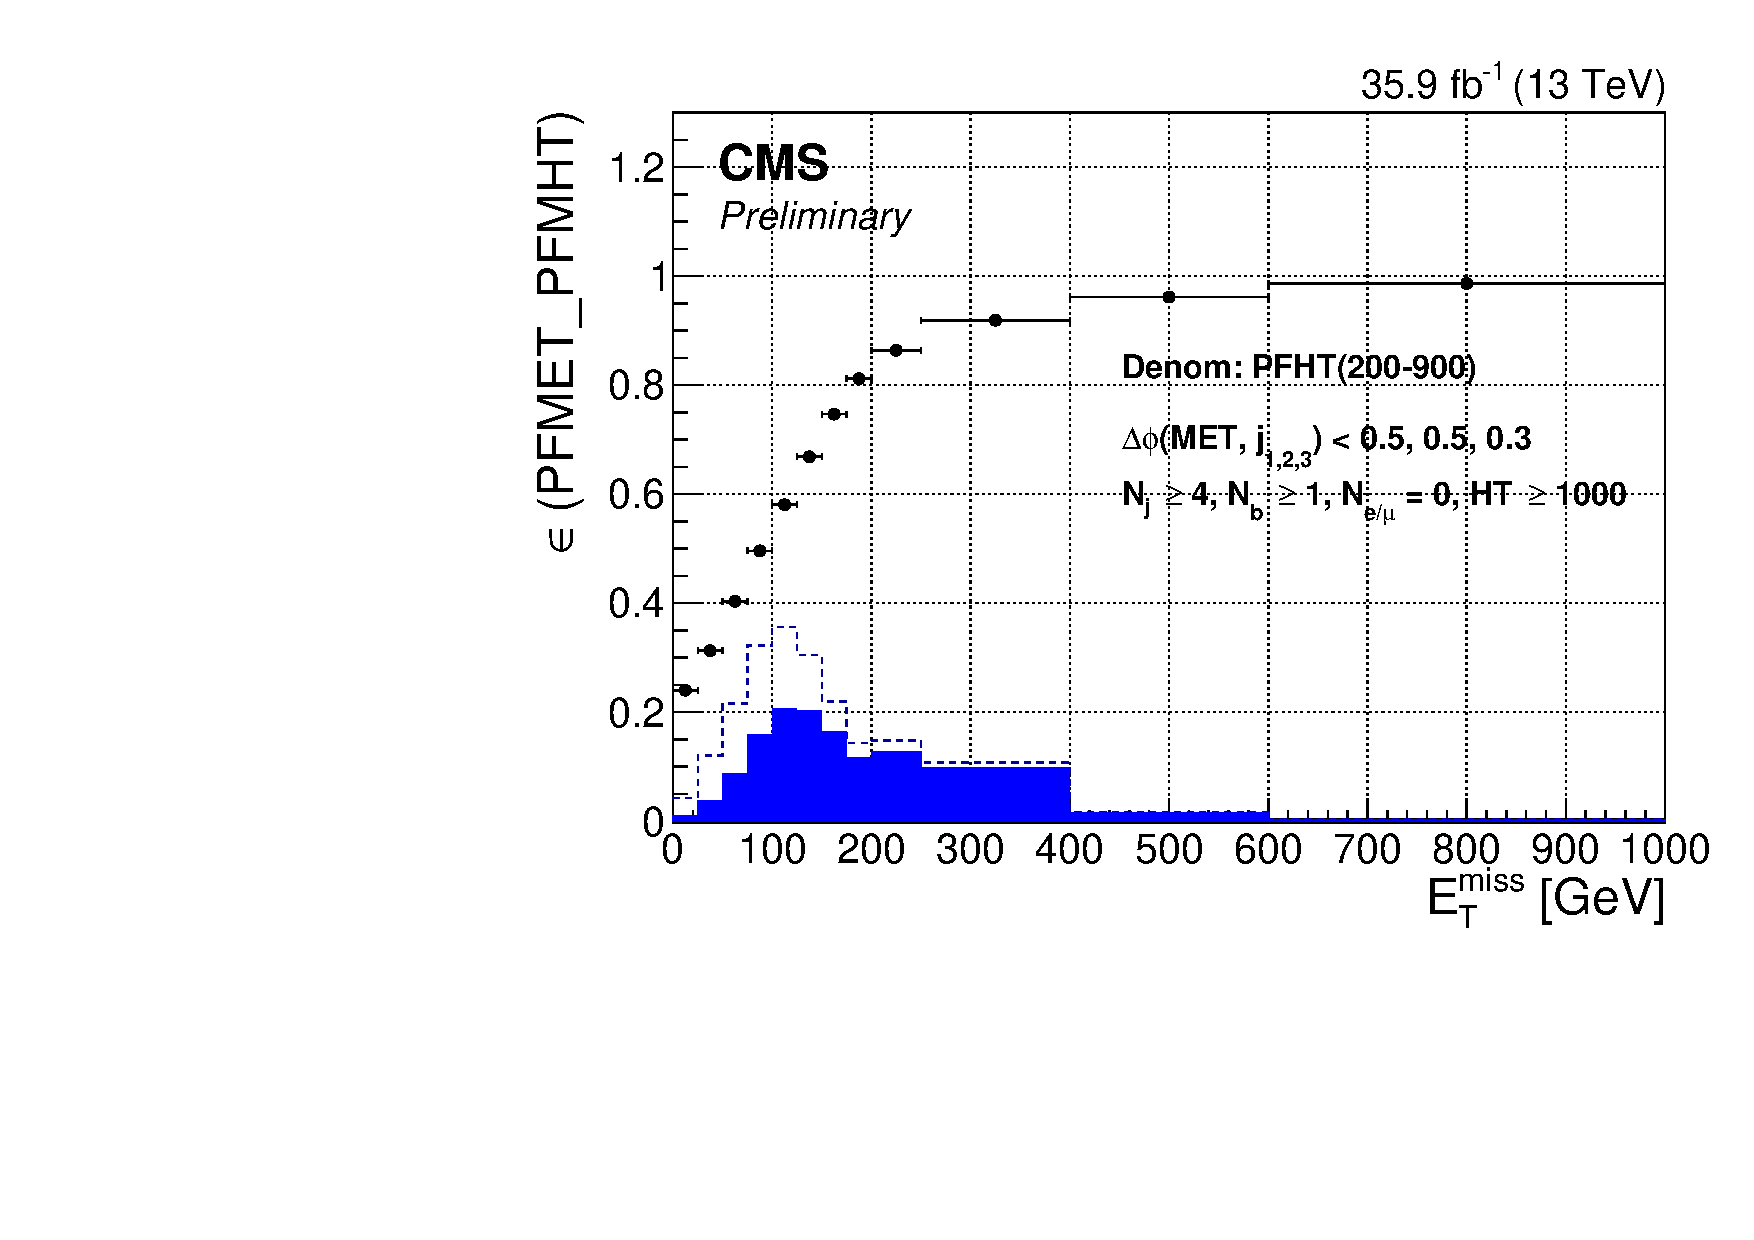
\includegraphics[width=0.49\linewidth]{sections/mc4/EvtSelSBOpt/figures/TrigHT_QCD_TrigMET_HTMore1000_9.pdf}
   \caption{ The trigger efficiency, denote by the black point, as a function
   of the offline \MET for (left) 300 $< \HT <$ 1000 and (right) $\HT >$ 1000.
   The error bar indicates the statistical uncertainty of the trigger
   efficiency. The dash blue line represents the denominator passing the
   selection, while the solid blue histogram represents the numerator where
   the denominator events also trigger the search triggers. }
   \label{fig:TrigMETQCD}
 \end{center}
\end{figure}

Events in the di-muon control sample, which is used for the estimation of the
background from events in which a Z boson decays into neutrinos, are
collected by the single muon trigger. 
\begin{itemize}
  \item \texttt{HLT\_IsoMu24\_eta2p1\_v*}.
  \item \texttt{HLT\_IsoTKMu24\_eta2p1\_v*}.
  \item \texttt{HLT\_Mu50\_eta2p1\_v*}.
\end{itemize}
The trigger efficiencies are measured in the single-electron sample with below selections:
\begin{itemize}
  \item Pass all filters
	\item Leading reconstructed electron with $p_{T}>$ 30GeV
  \item At least one reconstructed muon
  \item $\njets\geq4$
  \item \nbjets $\ge$ 1
  \item \HT $\ge$ 300 GeV
\end{itemize}

The measured single muon trigger efficiency as a function of the reconstructed
leading muon $p_{T}$ and $\eta$ is shown in Fig.~\ref{fig:TrigMuon}.
The muon trigger efficiency is also measured in the HT and MET dataset as
cross checks. We also checked the benefits of adding the double muon triggers
\begin{itemize}
  \item \texttt{HLT\_Mu17\_TrkIsoVVL\_Mu8\_TrkIsoVVL\_DZ\_v*}.
  \item \texttt{HLT\_Mu17\_TrkIsoVVL\_TkMu8\_TrkIsoVVL\_DZ\_v*}.
\end{itemize}.
We do observe a small gain of muon efficiencies as shown in
Fig.~\ref{fig:TrigMuon}, but no beneficial for the $Z \rightarrow \nu \nu$ background method.

\begin{figure}[tbp]
 \begin{center}
   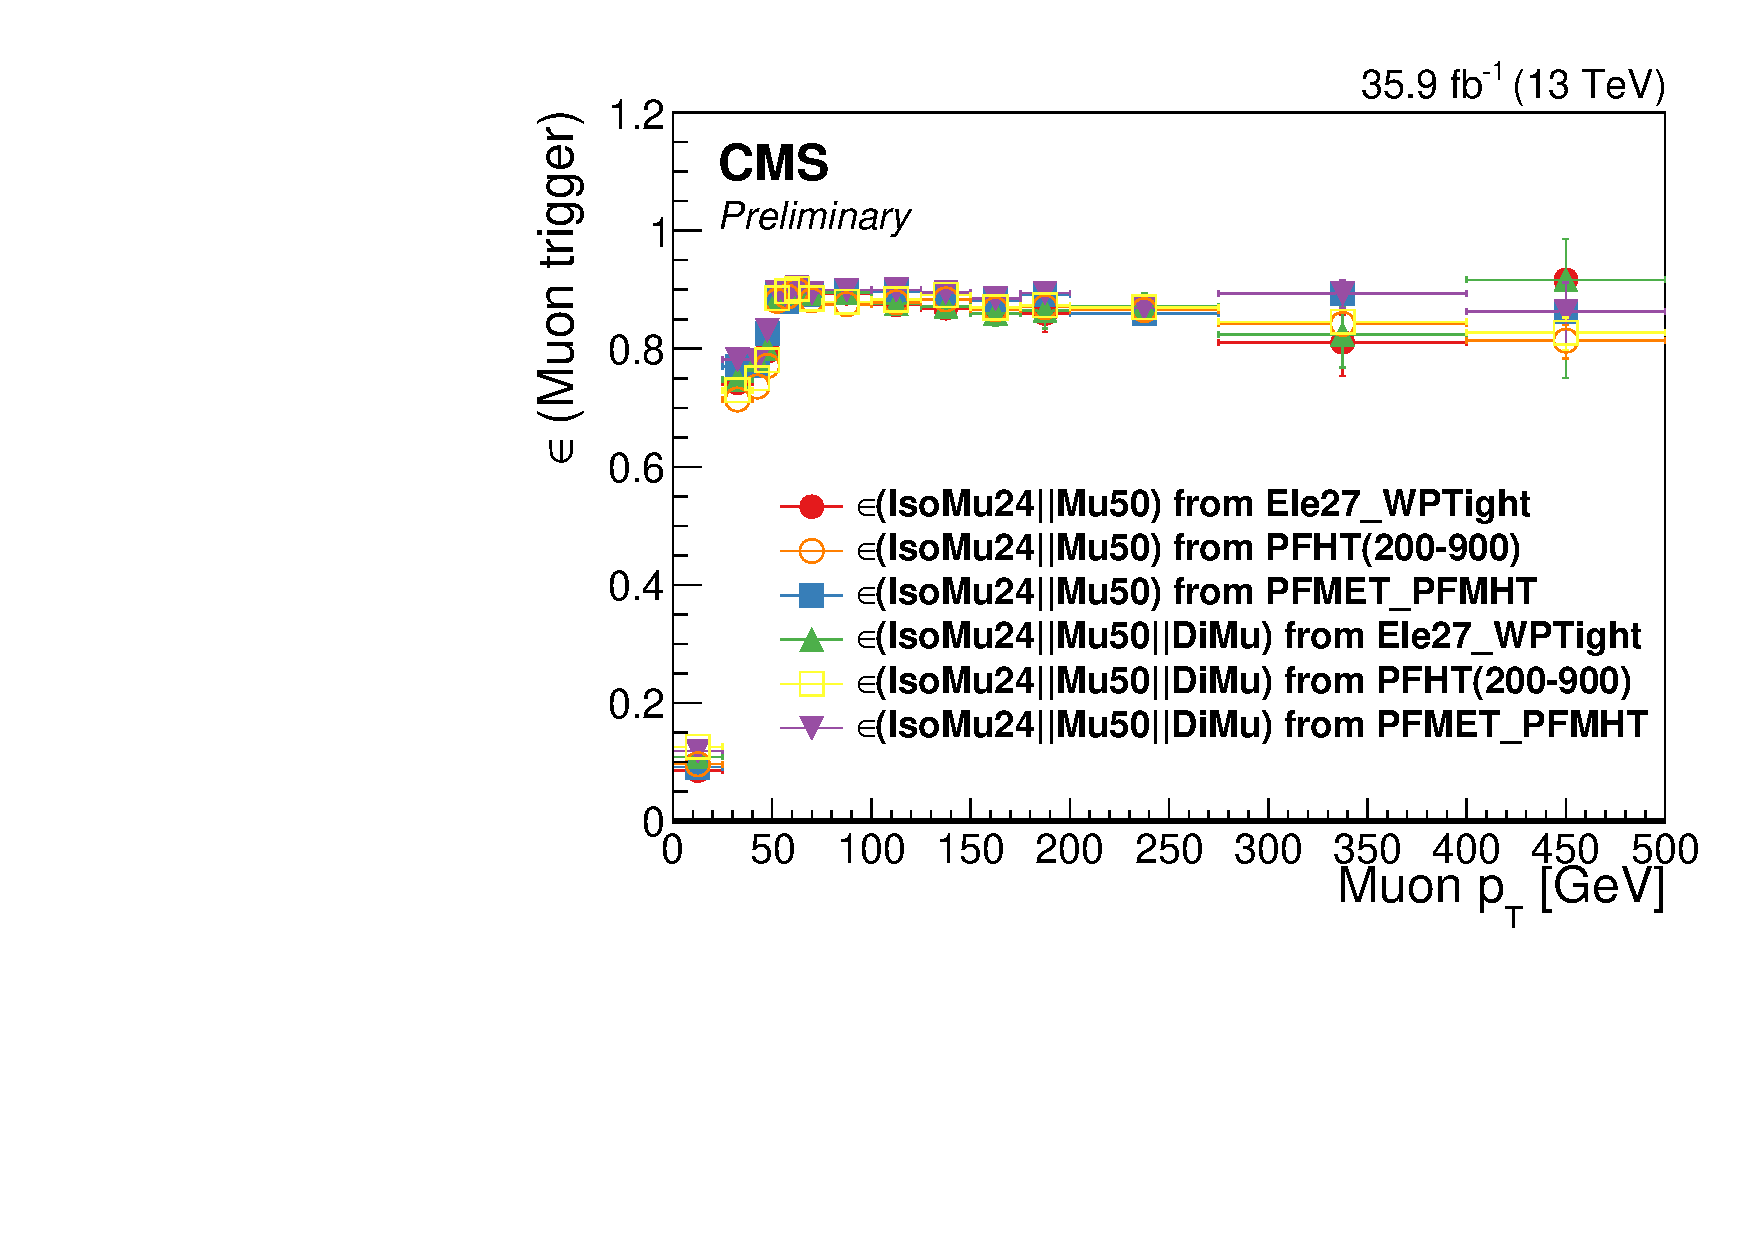
\includegraphics[width=0.49\linewidth]{sections/mc4/EvtSelSBOpt/figures/MuonPT.pdf}
   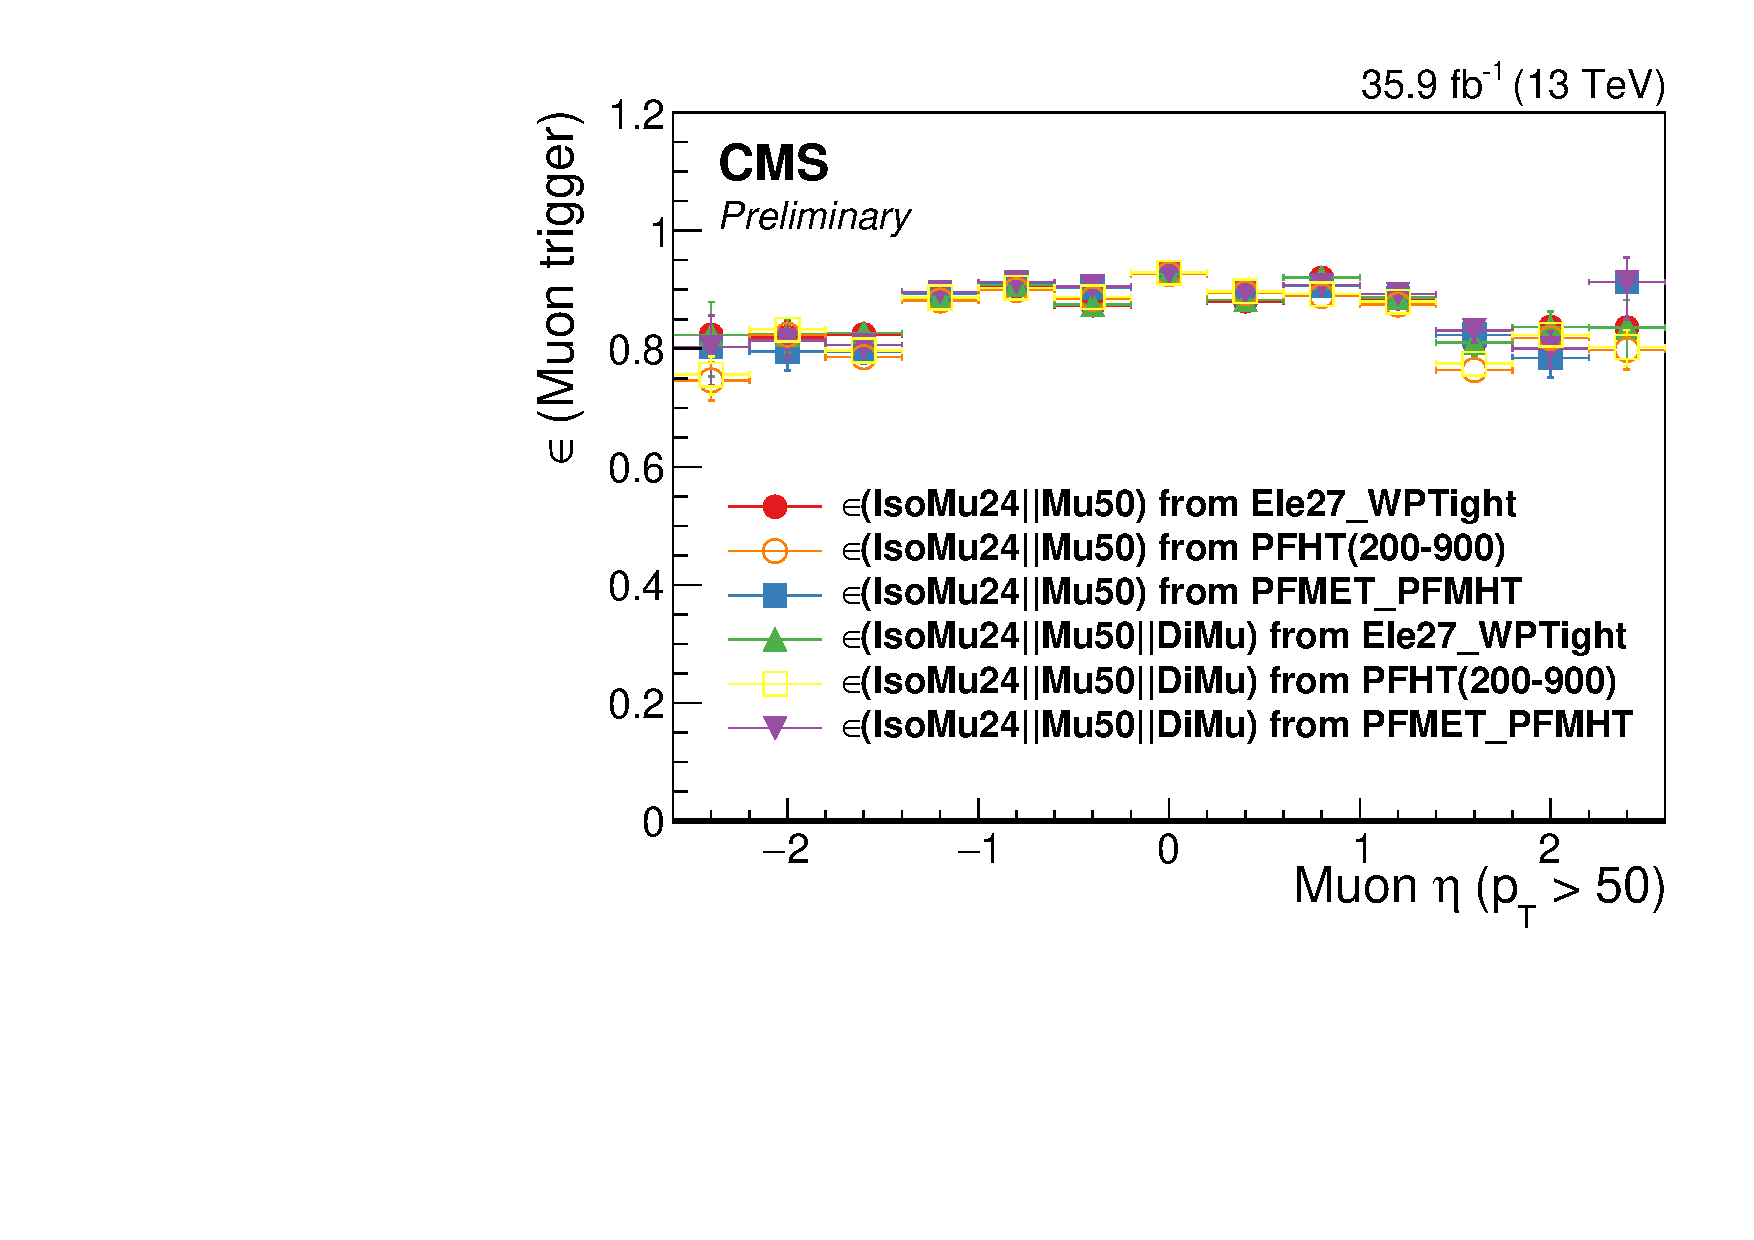
\includegraphics[width=0.49\linewidth]{sections/mc4/EvtSelSBOpt/figures/MuonEta.pdf}
   \caption{ The trigger efficiency as a function of the offline leading Muon
	 (left) $p_{T}$ and (right) $\eta$.}
   \label{fig:TrigMuon}
 \end{center}
\end{figure}

We also checked the trigger efficiency as a function of number of AK4 jets and
$b$-tagged jets, after requiring leading muon with $p_{T}>$ 50GeV, as shown in
Fig.~\ref{fig:TrigMuonJets}. We observed similar efficiency from different
measurements.
\begin{figure}[tbp]
 \begin{center}
   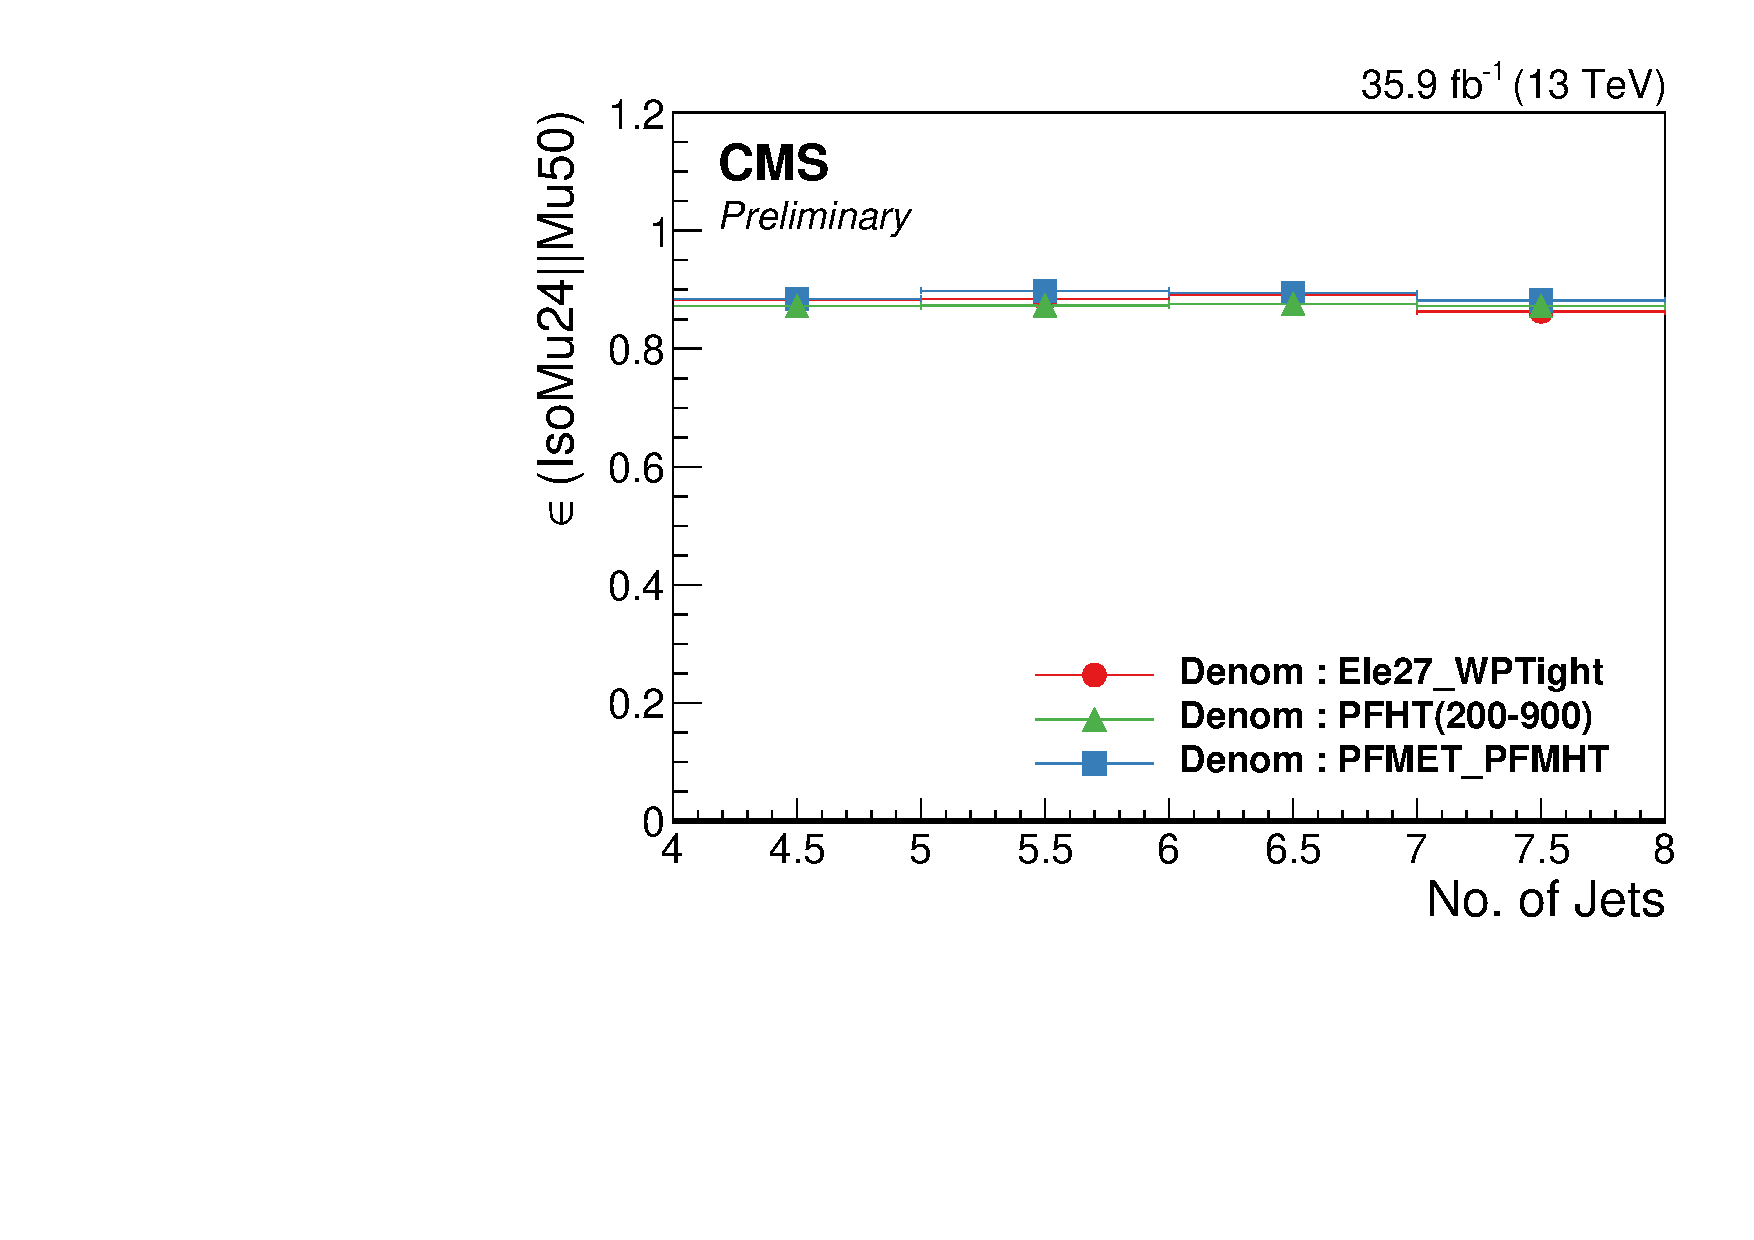
\includegraphics[width=0.49\linewidth]{sections/mc4/EvtSelSBOpt/figures/MuonNJets.pdf}
   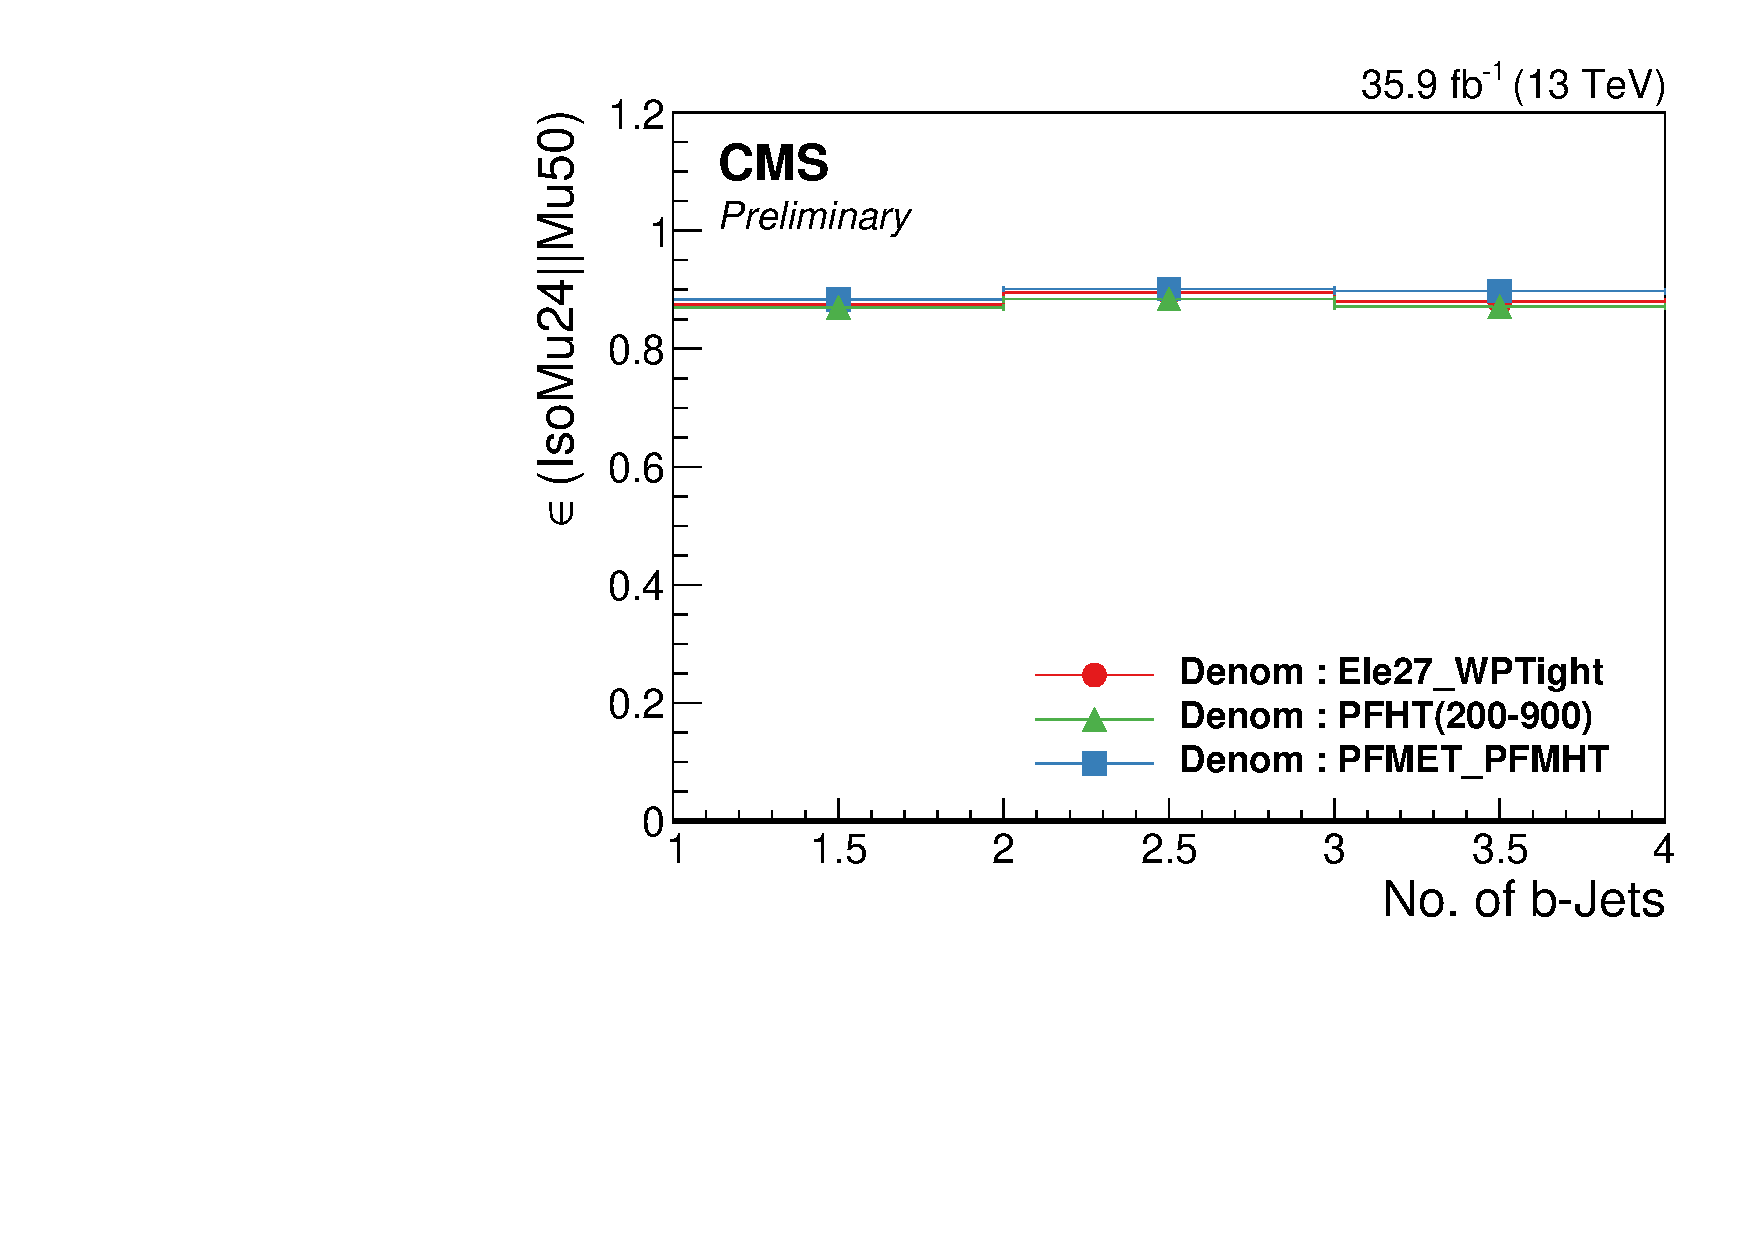
\includegraphics[width=0.49\linewidth]{sections/mc4/EvtSelSBOpt/figures/MuonNBs.pdf}
   \caption{ The trigger efficiency as a function of the offline (left) number
		 of jets with $p_{T}>$ 30 GeV and (right) number of $b$-tagged jets with $p_{T}$
		 $>$ 30GeV, with leading reconstructed muon $p_{T}$ above 50GeV from the
   single-muon trigger. The red point denote the measurement from
   single-electron dataset. The green triangle represents measurement from HT
   dataset, while blue square represents measurement from MET dataset.}
   \label{fig:TrigMuonJets}
 \end{center}
\end{figure}

\subsection{Pre-selection}
\label{sec:pre-selection}

The search looks at multijet events, with b-jets decaying from top quarks, 
large \MET and no leptons. Initially, a loose baseline selection is applied 
in \MET, \HT, \njets and \nbjets. %As illustrated in Tab.~\ref{tab:cutflowMC}, 
This baseline selection preserves 2-20\% of the signal events. 
The events passing the baseline selection are classified into search regions
defined in terms of \ntops, \nbjets, \MET, \HT and \MTTwo.

The following cuts define the baseline selection:

\begin{itemize}
\item Pass all filters that remove detector- and beam-related noise: 
  \begin{itemize}
    \item HBHE noise filter, 
    \item HBHEiso noise filter, 
    \item Ecal dead cell trigger primitive filter,
    \item Primary vertex filter,
    \item Bad EE super crystal filter,
    \item Global tight beam halo filter,
%    \item Fourth bad EE super crystal filter,
    \item Bad muon filter,
    \item Bad charged hadron filter,
    \item Loose JetID event filter.
  \end{itemize}

\item $\njets\geq4$:

%Since the stop is produced in pairs (R-parity conservation) and each one decays to two top quarks, the all-hadronic final state must contain at least four jets. 
Since the stop is produced in pairs and each stop decays to a top and a LSP, the all-hadronic final state will contain 6 jets. Not all the jets pass the selection cuts, therefore we only require at least four jets.
Jets are reconstructed with the Particle Flow (PF) technique
and clustered with the anti-$k_\mathrm{T}$ algorithm with a resolution 
parameter D=0.4~\cite{Cacciari:2008gp} (AK4). Every jet
is required to have $p_{T}>$30 GeV and $|\eta|<$2.4. In addition, they must 
pass the loose jet ID criteria for PF jets as recommended by the JetMET group. 
If any of the jets fail the loose jet ID criteria, the event
is rejected (referred to as the loose JetID event filter
above).

The leading two jets are required to have 
$p_{T}>$50 GeV since SUSY predicts centrally produced jets with 
high $p_{T}$.

\item \MET $\ge$ 250 GeV, where we use the type1-corrected PFmet, using the Summer16\_23Sep2016V3 jet energy corrections and the cut threshold is constrained by trigger
efficiency requirements.

\item \MTTwo $\ge$ 200 GeV, which is mainly used to reduce SM background events with low value of \MTTwo. Especially it works well for the 
\ttbar events where the \MTTwo shows a kinematic edge around the top quark mass.

\item \HT $\ge$ 300 GeV, with \HT = $\sum_{\mathrm{jets}} p_{T}$ where the $p_{T}$ is the magnitude.
Jets in the \HT calculation must meet the same jet seletion criteria defined above.

\item \nbjets $\ge$ 1, with b-jets identified using the CSV b-tagging algorithm 
(CSVM), medium working point.

\item Muon veto:

Muon candidates are selected using the ``Medium Muon" selection~\cite{POGmuon},
recommended by the muon Physics Objects Group (POG).
Muon candidates satisfy $p_{T}>10$ GeV and $|\eta|<2.4$.
Details of the muon medium ID criteria are listed in the Table~\ref{tab:MuonMediumID} and Table~\ref{tab:MuonMediumIDGoodGlobalMuon}.
In addition to the official medium selection, we also apply the additional impact parameter cut to select muon candidate, details listed in the Table~\ref{tab:MuonMediumIDImpactParameter}.
%Note that there are multiple places with the words "2016 ICHEP". This is precisely because SUSY PAG recommends to keep using IDs from ICHEP therefore we label them accordingly with "2016 ICHEP".
%  The recommended PF relative-isolation criterion
%  with $\delta\beta$-based corrections and $\Delta R = 0.4$ is used with
%  a ``loose" cut of $< 0.20$ to eliminate events with an isolated muon.
A PF relative-isolation criteria is enforced (mini-isolation), for which the
the isolation cone shrinks as a function of increasing muon $p_{T}$. The $p_{T}$ 
in the mini-isolation cone is required to be less than 20\% of the 
muon $p_{T}$ to eliminate events with an isolated muon. 
%\fixme{Update to new recommended medium WP to come soon.}

\newsavebox{\closureBox}

\begin{table}[htbp]
\fontsize{10 pt}{1.2 em}
\selectfont
\begin{centering}
\caption{\label{tab:MuonMediumID} Muon Medium ID 2016 HIP Safe}
\hspace*{-4ex}
\begin{lrbox}{\closureBox}
\begin{tabular}{|c|c|}
\hline
  Muon Medium ID                                      &               \\
\hline
  Loose muon ID                                       & Yes           \\
\hline
  Fraction of valid tracker hits $>$                  & 0.80          \\
\hline
  Good Global muon OR Tight segment compatibility $>$ & Yes OR 0.451 \\
\hline
\end{tabular}
\end{lrbox}
\scalebox{0.80}{\usebox{\closureBox}}
\par\end{centering}
\end{table}

\begin{table}[htbp]
\fontsize{10 pt}{1.2 em}
\selectfont
\begin{centering}
\caption{\label{tab:MuonMediumIDGoodGlobalMuon} Muon Medium ID HIP Safe Good Global Muon}
\hspace*{-4ex}
\begin{lrbox}{\closureBox}
\begin{tabular}{|c|c|}
\hline
  Good Global muon                      &       \\
\hline
  Global muon                           & Yes   \\
\hline
  Normalized global-track $\chi^{2} <$  & 3     \\
\hline
  Tracker-Standalone position match $<$ & 12    \\
\hline
  Kick finder $<$                       & 20    \\
\hline
  Segment compatibility $>$             & 0.303 \\
\hline
\end{tabular}
\end{lrbox}
\scalebox{0.80}{\usebox{\closureBox}}
\par\end{centering}
\end{table}

\begin{table}[htbp]
\fontsize{10 pt}{1.2 em}
\selectfont
\begin{centering}
\caption{\label{tab:MuonMediumIDImpactParameter} Additional Impact Parameter cut on Muon }
\hspace*{-4ex}
\begin{lrbox}{\closureBox}
\begin{tabular}{|c|c|}
\hline
  Muon Impact Parameter &     \\
\hline
  d0 $<$                & 0.2 \\
\hline
  dz $<$                & 0.5 \\
\hline
\end{tabular}
\end{lrbox}
\scalebox{0.80}{\usebox{\closureBox}}
\par\end{centering}
\end{table}

\item Electron veto:

Electron candidates are selected using the POG-recommended
``Cut Based VETO" selection. 
Different cut criteria are applied on the barrel and endcap electromagnetic calorimeter region, values of the cut based veto are listed in the Table~\ref{tab:ElectronCutBasedVeto}. 

They are required to have $p_{T}>10$ GeV and $|\eta|<2.5$.
reconstructed Isolated electrons are rejected using PF-based "mini-isolation" cut requiring
less than 10\% of the electron energy in the isolation cone.

\begin{table}[htbp]
\fontsize{10 pt}{1.2 em}
\selectfont
\begin{centering}
\caption{\label{tab:ElectronCutBasedVeto} Electron Cut Based Veto 2016 Data in 80X CMSSW offline reconstruction condition}
\hspace*{-4ex}
\begin{lrbox}{\closureBox}
\begin{tabular}{|c|c|c|}
\hline
                                     & ECAL Barrel($|Eta|<1.479$) & ECAL Endcap($|Eta|>1.479$) \\
\hline
  full5x5 sigmaIetaIeta $<$          & 0.0115                     & 0.037                    \\
\hline
  abs(dEtaInSeed) $<$                & 0.00749                    & 0.00895                  \\
\hline
  abs(dPhiIn) $<$	             & 0.228                      & 0.213                    \\
\hline
  H/E $<$	                     & 0.356                      & 0.211                    \\
\hline
  Rel. comb. PF iso with EA corr $<$ & 0.175                      & 0.159                    \\
\hline
  abs(1/E-1/p) $<$                   & 0.299                      & 0.15                     \\
\hline
  expected missing inner hits $<$    & 3                          & 4                        \\
\hline
  pass conversion veto               & yes                        & yes                      \\
\hline
\end{tabular}
\end{lrbox}
\scalebox{0.80}{\usebox{\closureBox}}
\par\end{centering}
\end{table}

\item Angular cut:

A cut on the angle between \MET and the first three leading jets, 
$\Delta\phi(\MET, j_{1,2,3})>$ 0.5, 0.5, 0.3, is applied to remove 
events coming from QCD processes.

\item Isolated track veto:

After applying the cuts described above
the residual background comes from
\ttbar, single top, and $W+$jets events with one $W\rightarrow l\nu$
decay where $l$ can be an electron, muon or tau decaying hadronically. 
To further suppress these backgrounds, we reject events 
that have one or more isolated tracks. The track isolation
is calculated from charged PF candidates consistent with the 
reconstructed primary vertex ($|dz(PV)|<0.1~\mathrm{cm}$).
The requirements are different for muon, electron and charged hadron tracks.
For both electron and muon tracks, the isolated track requirements are: 
$p_{T}>$5 GeV, $|\eta|<$2.5 and relative isolation less than 0.2.
For charged hadron tracks, the $p_{T}$ requirement
is raised to be at least 10 GeV and the relative isolation value to be less 
than 0.1. To retain more signal, and thus improve signal-to-background
event discrimination, events with one isolated track, as defined
above, are only rejected if they satisfy
  \begin{equation}
    \label{eq:mt_isotk}
    m_T(tk,\MET) = \sqrt{2p_{T}^{tk}\MET(1-\cos\Delta\phi)}<100\;\mathrm{GeV}
  \end{equation}
  where $p_{T}^{tk}$ is the transverse momentum of the track and
  $\Delta\phi$ is the azimuthal separation between the track and \MET
  vector. 

\end{itemize}

\subsection{Search regions}
\label{sec:searchregions}

In our 2016 analysis, we bin the search regions in terms of the number of b-tagged jets and top candidates. 
The top reconstruction and identification procedure (top-tagging) 
is described in Sec.~\ref{sec:top-tagging}. 

In order to improve background suppression, in particular the \ttbar
contribution, the \MET, \HT and \MTTwo variables were added to the 
set that defines the search regions. The variable 
\MTTwo~\cite{Lester:1999tx,Barr:2003rg} is an extension of the transverse 
mass variable that is sensitive to the pair production of heavy particles, each
of which decays to an invisible particle.
The \pTop, the \pRsystem, and the \MET in an event
are used to constructed \MTTwo assuming the invisible particles are massless.
In order to illustrate how the \MTTwo is calculated, let us take the process 
${\rm pp} \rightarrow \sTop\santiTop\rightarrow t\bar{t}\chi_1^0\chi_1^0$
as an example. This process contains two simultaneous decays of an unseen 
particle of unknown mass(\sTop or \santiTop) into another invisible 
particle ($\chi_1^0$) and visible particle ($t$ or $\bar{t}$). The
variable \MTTwo is defined as:
\begin{equation} \label{eq:MT2}
   \begin{array}{l}
     \displaystyle{ \MTTwo \equiv \min_{\vec{q}_{T}^{(1)}+\vec{q}_{T}^{(2)} = \vec{p}_{T}} [\max\{m_{T}^2(\vec{p}_{T}^{t^{(1)}}, \vec{q}_{T}^{(1)}; m_{\chi_1^0}), m_{T}^2(\vec{p}_{T}^{t^{(2)}}, \vec{q}_{T}^{(2)}; m_{\chi_1^0})\}]  } 
   \end{array}
\end{equation}
where the $m_{T}^2$ is the transverse mass,
\begin{equation} \label{eq:MTdef}
   \begin{array}{l}
     \displaystyle{
        m_{T}^2(\vec{p}_{T}^{t^{(1)}}, \vec{q}_{T}^{(1)}; m_{\chi_1^0}) \equiv m_{t^{(1)}}^{2} + m_{\chi_1^0}^2 + 2(E_{T}^{t^{(1)}}E_{T}^{(1)} - \vec{p}_{T}^{t^{(1)}} \cdot \vec{q}_{T}^{(1)})
     }
   \end{array}
\end{equation} 
\MTTwo is a minimization of two transverse masses with a constraint that 
the sum of the transverse momenta of both $\chi_1^0$'s is equal to the 
missing transverse momentum of the event, i.e., 
$\vec{q}_{T}^{(1)}+\vec{q}_{T}^{(2)} = \vec{p}_{T}$. 
\MTTwo has a kinematic upper limit which is the \sTop mass. 
The superscripts $(1)$ and $(2)$ in the equations refer to the individual 
decays of the \sTop particles. In the specific case of the analysis described
in this note, we replace the quantities related to superscript $(1)$ by those
of associated with the fully reconstructed top quark, i.e., the \pTop. 
Similarly, we replace the quantities related to superscript $(2)$ by those
of the partially reconstructed top quark, i.e., the \pRsystem 
for $\ntops =1$ and the fully reconstructed top quark for $\ntops \ge 2$. 
\MET then corresponds to $\vec{p}_{T}$ in the equation~\ref{eq:MT2}. 
Since we assume that the invisible particle is massless, $m_{\chi_1^0}$ should 
be zero in Eqs.~\ref{eq:MT2}-~\ref{eq:MTdef}. 

In a few words, we start from the fact that there is at least one good hadronic top candidate in the search samples. 
If there are two top candidates, \MTTwo is calculated using the pair of top 
candidates and \MET. In case of there are more than two top candidates
in the sample, we compute \MTTwo for all combinations and choose the 
\MTTwo with the smallest value. If there is only one top candidate identified
by the top-tagging algorithm, we reconstruct the other top 
quark from the remanent of the event using the b-tagged jet (or the hardest $p_{T}$ jet if no b-tagged jet found) as a seed and the R-sys 
jet closest to the seed jet with an invariant mass between 50 GeV and 
the top quark mass. In case no combination satisfies the invariant mass
requirement, we use the seed jet as the only remanent of the other 
top quark. In the latter case, \MTTwo is calculated from the reconstructed top candidate, the remanent and the \MET.

%Table~%\ref{tab:cutflowMC} 
%illustrates on the sample selection process with
%a MC simulation. The cut flow is shown, as well as the predictions for the
%different SM backgrounds. Table~%\ref{tab:cutflowMCSat} 
%illustrates on the sample selection process with
%a few signal points as well as the total MC.

%\begin{landscape}
%\newsavebox{\cutflowBox}
%\begin{table}[htb]
%  \caption{Sample selection cut flow and event yields from MC simulated 
%samples. All numbers are normalized to $12.9\fbinv$. 
%}
%  \label{tab:cutflowMC}
%  \vskip-5ex
%  \begin{center}
%    \begin{lrbox}{\cutflowBox}
%\begin{tabular}{c | c | c | c | c | c | c | c}
%Cut     &	 $t\bar{t}$ 	&	 QCD  &	 $Z(\nu\nu)+jets$        &	 $W(l\nu)+jets$ 	&	 Single top 	&	 Rare      &	$ t\bar{t}Z$ \\
%\hline
%No Cut 	&	 7.58e+05 (100\%)	&	 1.29e+09 (100\%) &1.1e+06 (100\%) &2.43e+06 (100\%) & 5.99e+04 (100\%) & 3.24e+05 (100\%) &	 1.99e+03 (100\%) \\
%Noise Filters     &7.49e+05 (98.8\%)&1.27e+09 (98.4\%)&1.1e+06 (100\%) &2.4e+06  (98.8\%)& 5.91e+04 (98.7\%)	&	 3.2e+05  (98.8\%)	&	 1.96e+03 (98.5\%) \\
%$\mu$ Veto         & 4.84e+05 (64.6\%)&1.27e+09 (100\%) &1.1e+06 (100\%) &1.87e+06 (77.9\%)&3.92e+04 (66.3\%)	&	 1.78e+05 (55.6\%)	&	 1.32e+03 (67.3\%) \\
%$e$ Veto    & 3e+05 (62\%)&1.27e+09 (100\%) &1.09e+06 (99.1\%) &1.42e+06 (75.9\%)&2.49e+04 (63.5\%)	&	 9.21e+04 (51.7\%)	&	 901 (68.3\%) \\
%IsoTrkVeto         & 1.9e+05 (63.3\%)&1.22e+09 (96\%)  &1.07e+06 (98.2\%) &1.08e+06 (76.1\%)& 1.62e+04 (65\%)  	&	 6.83e+04 (74.2\%)	&	 689 (76.5\%) \\
%$N_{jets} \geq 4$       &1e+05 (52.6\%)	& 1.57e+07 (1.3\%) &5.85e+04 (5.46\%)  & 6.91e+04 (6.4\%)& 6.39e+03 (39.4\%)	&	 6.39e+03 (9.4\%) 	&	 571 (82.9\%) \\
%$N_{B-jets} \geq 1$   &7.96e+04 (79.6\%)& 3.07e+06 (19.6\%)& 1.11e+04 (19\%) &1.31e+04 (19\%)& 4.66e+03 (72.9\%)	&	 2.29e+03 (35.8\%)	&	 458 (80.2\%) \\
%$H_{T} \geq 500$  &2.55e+04 (32\%)&5.6e+05  (18.2\%) & 4.22e+03 (38\%) & 5.17e+03 (39.5\%)& 1.92e+03 (41.2\%)	&	 1.09e+03 (47.6\%)	&	 244 (53.3\%) \\
%$\textrm{\MET} \geq 200$ &9.71e+03 (38.1\%)&2.71e+04 (4.8\%) & 2.44e+03 (57.8\%) &2.21e+03 (42.7\%)&622  (32.4\%)	&385 (35.3\%)   &	 124 (50.8\%) \\
%$\Delta\phi$            &5.56e+03 (57.3\%)& 3.07e+03 (11.3\%)&1.77e+03 (72.5\%) &1.29e+03 (58.4\%)	&292  (46.9\%)	&212 (55.1\%)     & 95.5 (77\%) \\
%$N_{t}\geq 1$  &	 2.5e+03 (45\%)	&589 (19.2\%)	& 305 (17.3\%)	&223 (17.3\%)	&82.8  (28.4\%)	& 70.7 (33.3\%) & 50.4 (52.8\%) \\
%$\textrm{\MTTwo} \geq 200$ 	&1.6e+03 (64\%)	&513  (87.1\%)&266 (87.2\%)&180  (80.7\%)	&61.3 (74\%) & 50.3 (71.1\%) &	 43.7 (86.7\%) \\
%\hline
%Baseline                	&	 1.6e+03 	&	 513              	&	 266 	&	 180 	&	 61.3    	&	 50.3             	&	 43.7     \\
%\end{tabular}
%    \end{lrbox}
%    \scalebox{0.80}{\usebox{\cutflowBox}}    
%  \end{center}
%\end{table}
%\end{landscape}

%\begin{landscape}
%\newsavebox{\cutflowBoxSig}
%\begin{table}[htb]
%  \caption{Sample selection cut flow and event yields from MC simulated
%samples. All numbers are normalized to $12.9\fbinv$. These are for some signal samples.}
%  \label{tab:cutflowMC}
%  \vskip-5ex
%  \begin{center}
%    \begin{lrbox}{\cutflowBox}
%\begin{tabular}{c | c | c | c | c | c}
%Cut           	&	 Total MC         	&	 T1tttt(1500,100)	&	 T1tttt(1200,800)   	&	 T2tt(500,325)     	&	 T2tt(850,100) \\ 	
%\hline
%No Cut           &	 1.29e+09 (100\%) 	&	 166 (100\%)     	&	 659 (100\%)        	&	 2.03e+03 (100\%)  	&	 217 (100\%)\\ 	
%Noise Filters       &	 1.28e+09 (99\%)  	&	 163 (98.2\%)    	&	 651 (98.8\%)        	&	 2e+03    (98.5\%)	&	 214 (98.6\%)\\ 	
%$\mu$ Veto           	&	 1.28e+09 (100\%) 	&	 103  (63.1\%)   	&	 417 (64\%)	&	 1.53e+03  (76.5\%)	&	 171 (79.9\%)\\ 	
%$e$ Veto              	&	 1.27e+09 (99\%)  	&	 65.8 (68.9\%)   	&	 277 (66.4\%)	&	 1.17e+03  (76.5\%)	&	 135 (78.9\%)\\ 	
%IsoTrkVeto           	&	 1.22e+09 (96\%)  	&	 58.1 (88.3\%)   	&	 215 (77.6\%)	&	 943       (80.6\%)	&	 126 (93.3\%)\\ 	
%$N_{jets} \geq 4$        &	 1.6e+07 (1.3\%)  	&	 58.1 (100\%)    	&	 214 (99.5\%)	&	 850       (90.1\%)	&	 113 (89.6\%)\\ 	
%$N_{B-jets} \geq 1$   	&	 3.18e+06 (19.8\%)	&	 55.6 (95.7\%)   	&	 203 (94.9\%)	&	 685 (80.6\%)   	&	 92.9 (82.2\%)\\ 	
%$H_T \geq 500$  	&	 5.98e+05 (18.8\%)&55.6 (100\%)    & 183 (90.1\%)	&	 454  (66.3\%) 	&	 87.4 (94.1\%)\\ 	
%$\textrm{\MET} \geq 200$ 	&	 4.26e+04 (7.1\%) 	&	 53.3 (95.7\%)   	&	 122 (66.7\%)	&	 305  (67.2\%) 	&	 82.6 (94.5\%)\\ 	
%$\Delta\phi$            	&	 1.23e+04 (28.9\%)	&	 43.6 (81.8\%)   	&	 96.8 (79.3\%)	&	 192  (63\%) 	&	 74.7 (90.4\%)\\ 	
%$N_{t} \geq 1$      	&	 3.82e+03 (31\%)  	&	 39.5 (90.6\%) 	&	 88.2 (91.1\%)   	&	 109 (56.8\%)  	&	 48.6 (65.1\%)\\ 	
%$\textrm{\MTTwo} \geq 200$ 	&	 2.71e+03 (70.9\%)	&	 38.8 (98.3\%)	&	 82.8 (93.9\%)   	&	 87.5  (80.3\%)	&	 47.5 (97.7\%)\\ 	
%Baseline                	&	 2.71e+03         	&	 38.8 	&	 82.8 	&	 87.5 	&	 47.5 \\ 	
%\end{tabular}
%    \end{lrbox}
%    \scalebox{0.90}{\usebox{\cutflowBox}}
%  \end{center}
%\end{table}
%\end{landscape}

%\todo{Fig.~\ref{fig:compSBvars} are from 2015 data and MC for illustration purpose. They will be updated with 2016 data and MC samples later.}
Fig.~\ref{fig:compSBvars} 
shows the comparison between total SM backgrounds from simulation and several signal points for the four search bin variables after baseline cuts. We can clearly see all the variables have good discrimination power. Observed data are also shown and the total SM backgrounds are scaled to the same yield as data to ensure a shape comparison. %The same scale is applied to signals as well in addition to the ``$\times5$" or ``$\times10$" scales.

\begin{figure}[h]
  \begin{center}
    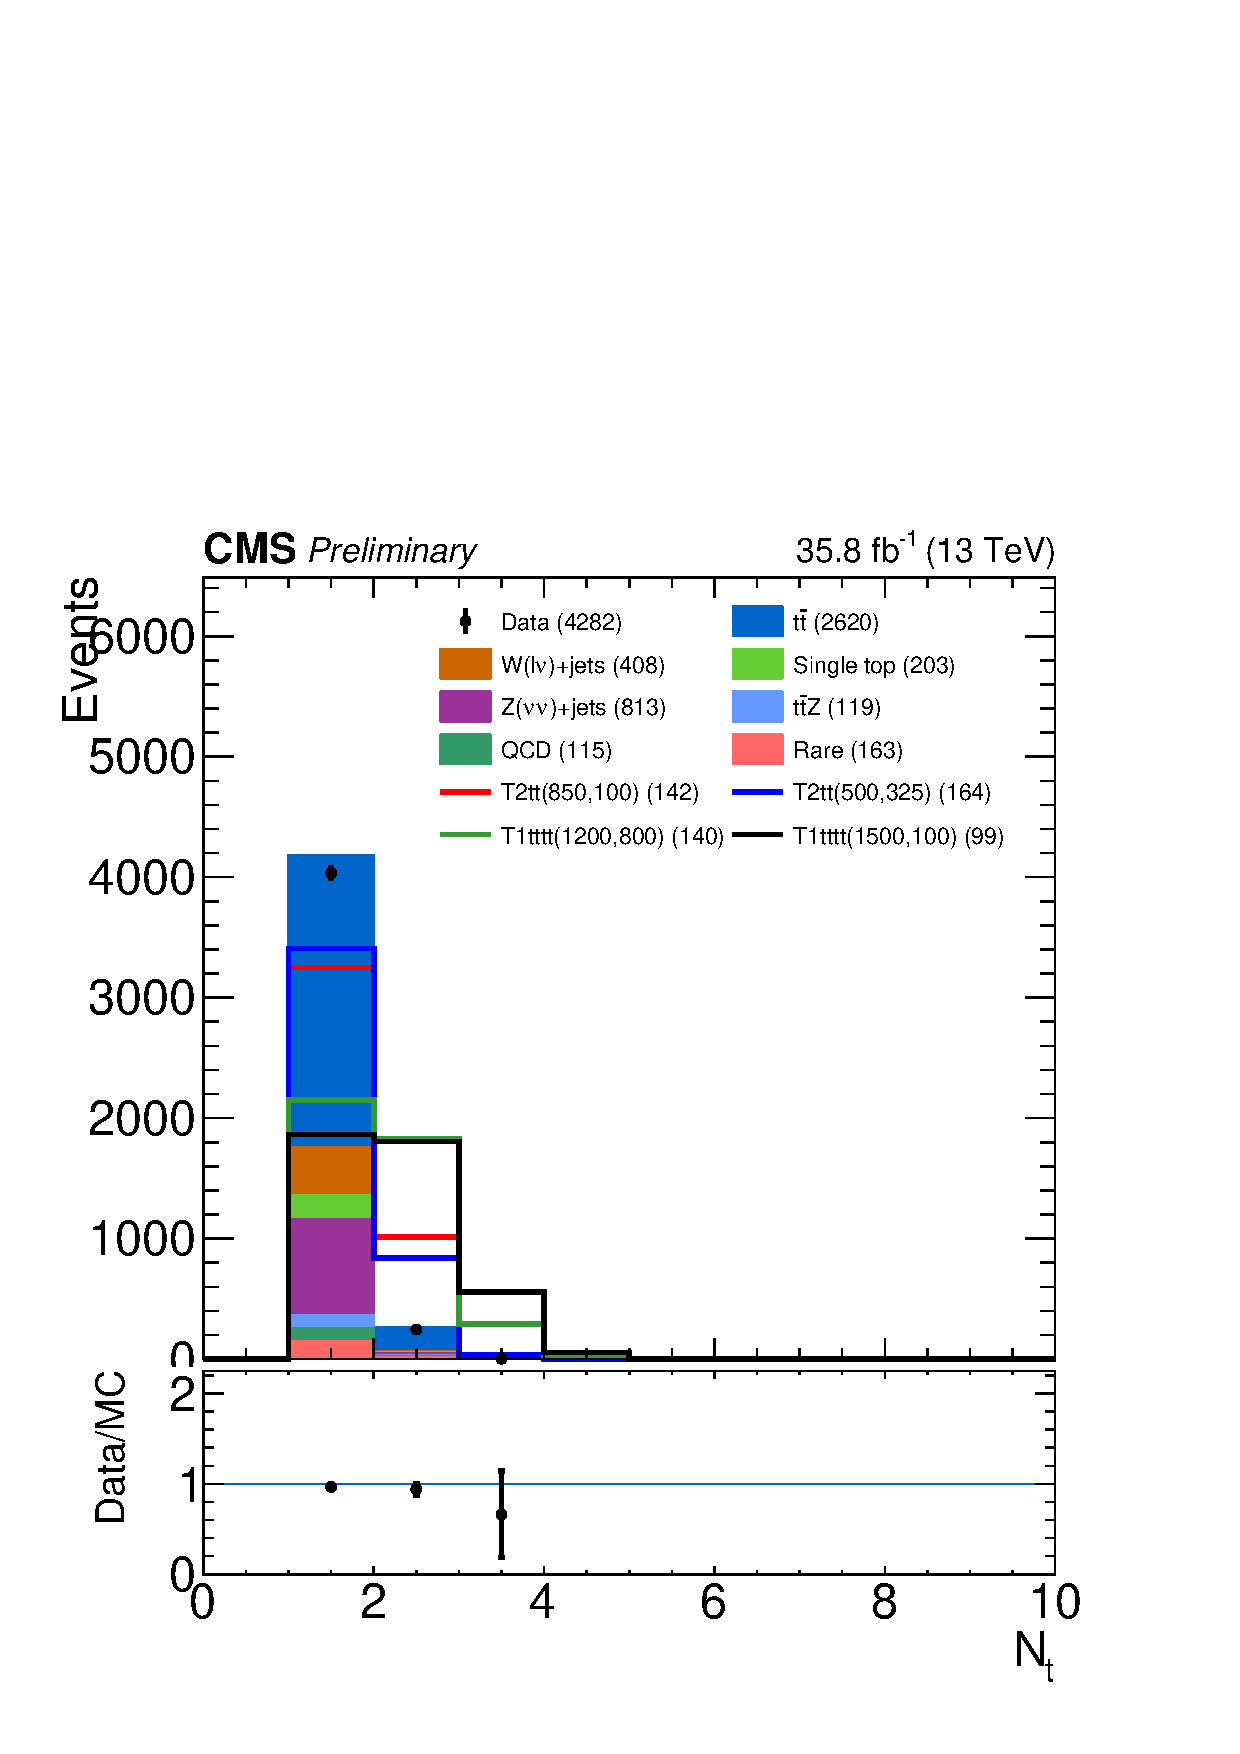
\includegraphics[width=0.45\linewidth]{sections/mc4/EvtSelSBOpt/figures/DataMC_MET_model_NTops_baseline.pdf}
    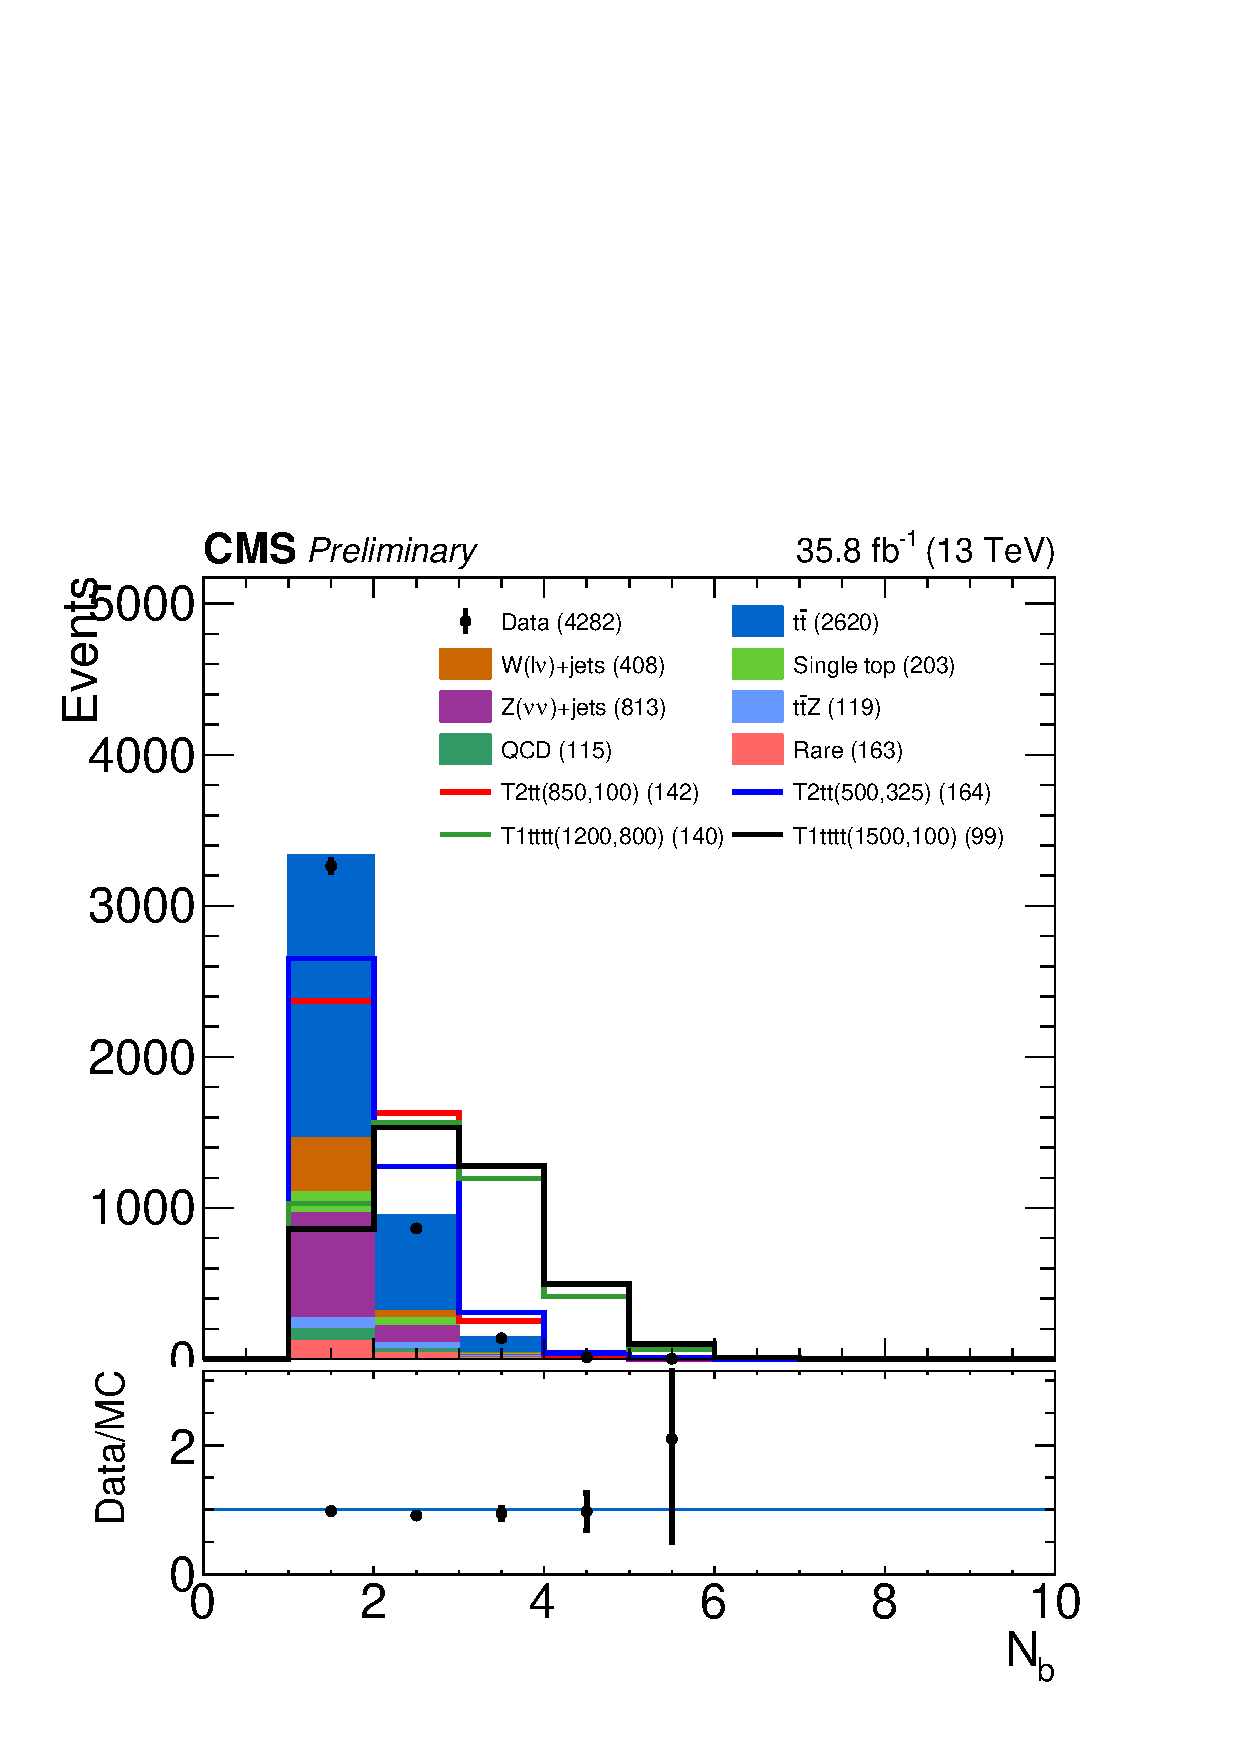
\includegraphics[width=0.45\linewidth]{sections/mc4/EvtSelSBOpt/figures/DataMC_MET_model_NBJEts_baseline.pdf}\\
    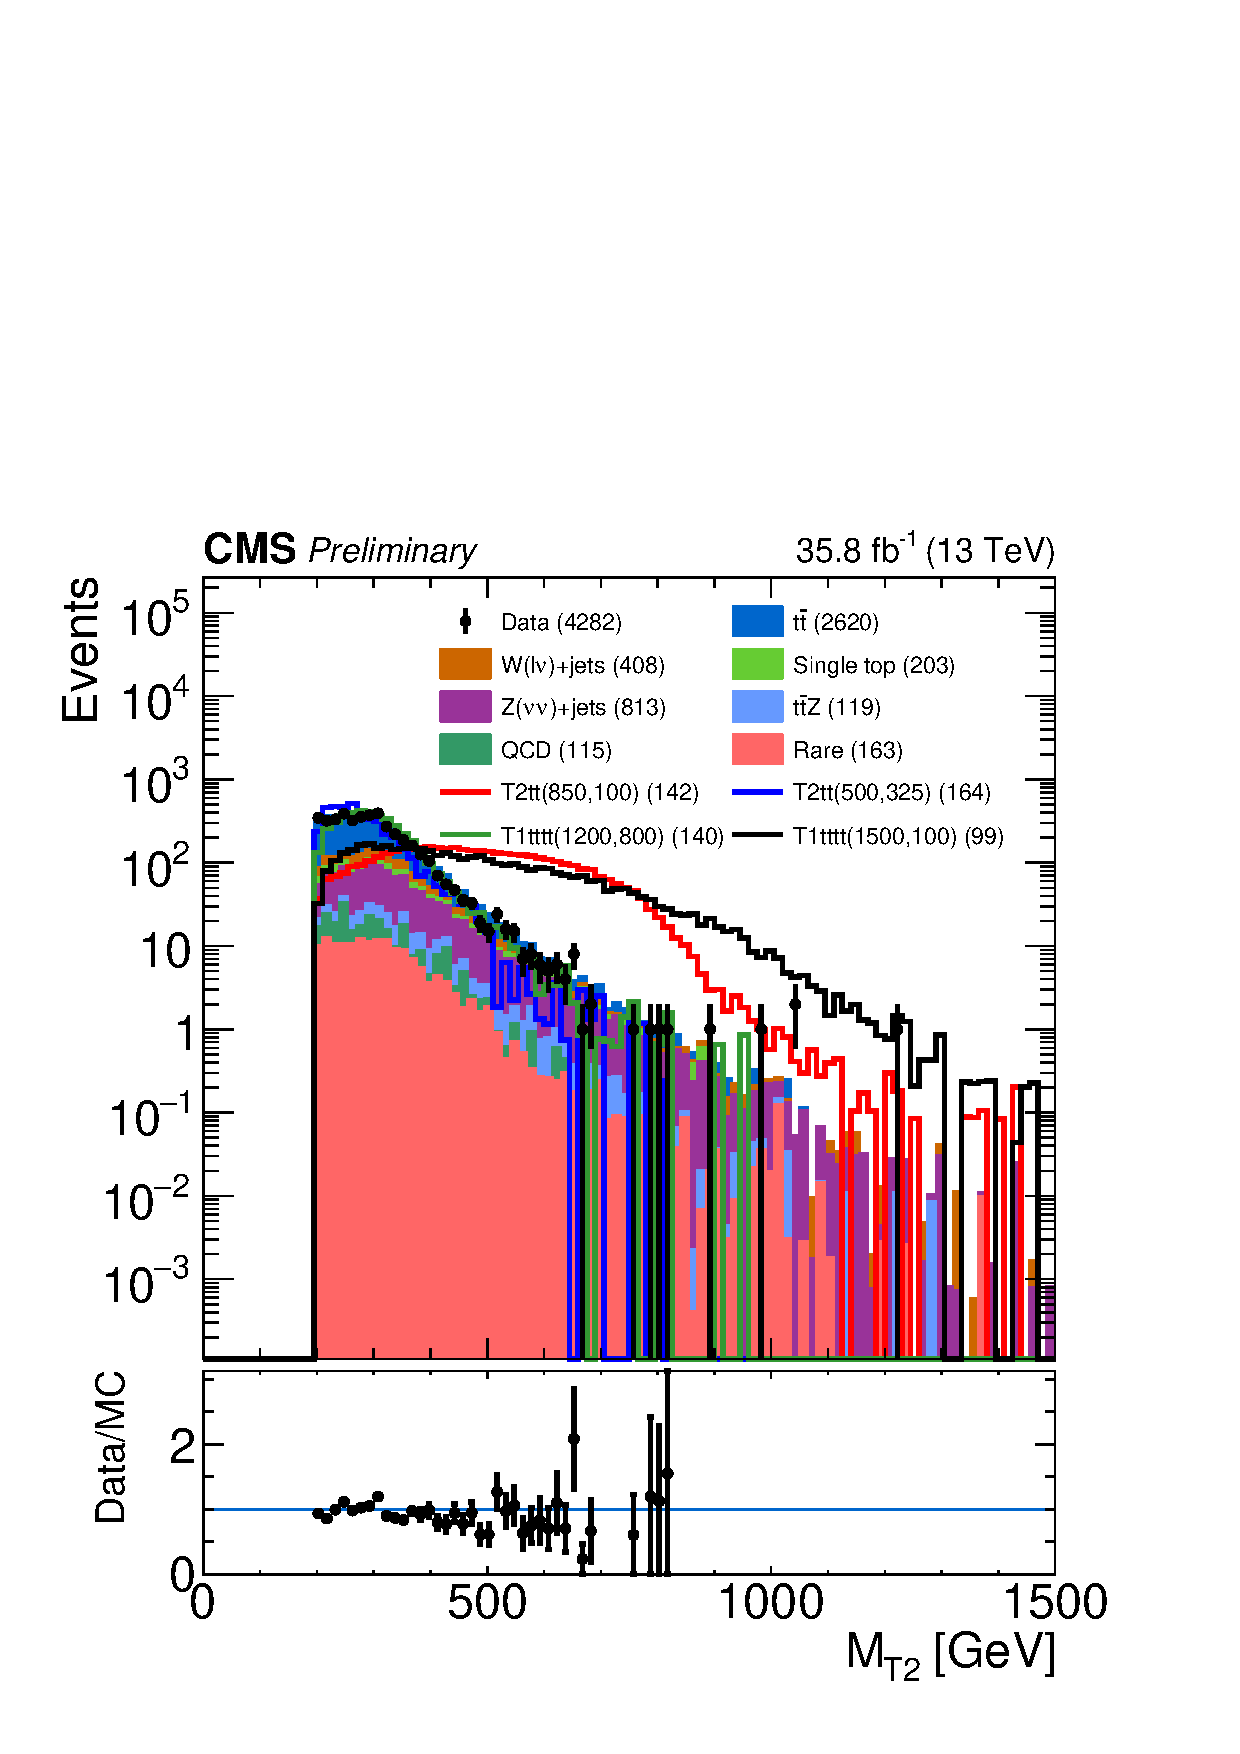
\includegraphics[width=0.45\linewidth]{sections/mc4/EvtSelSBOpt/figures/DataMC_MET_model_MT2_baseline.pdf}
    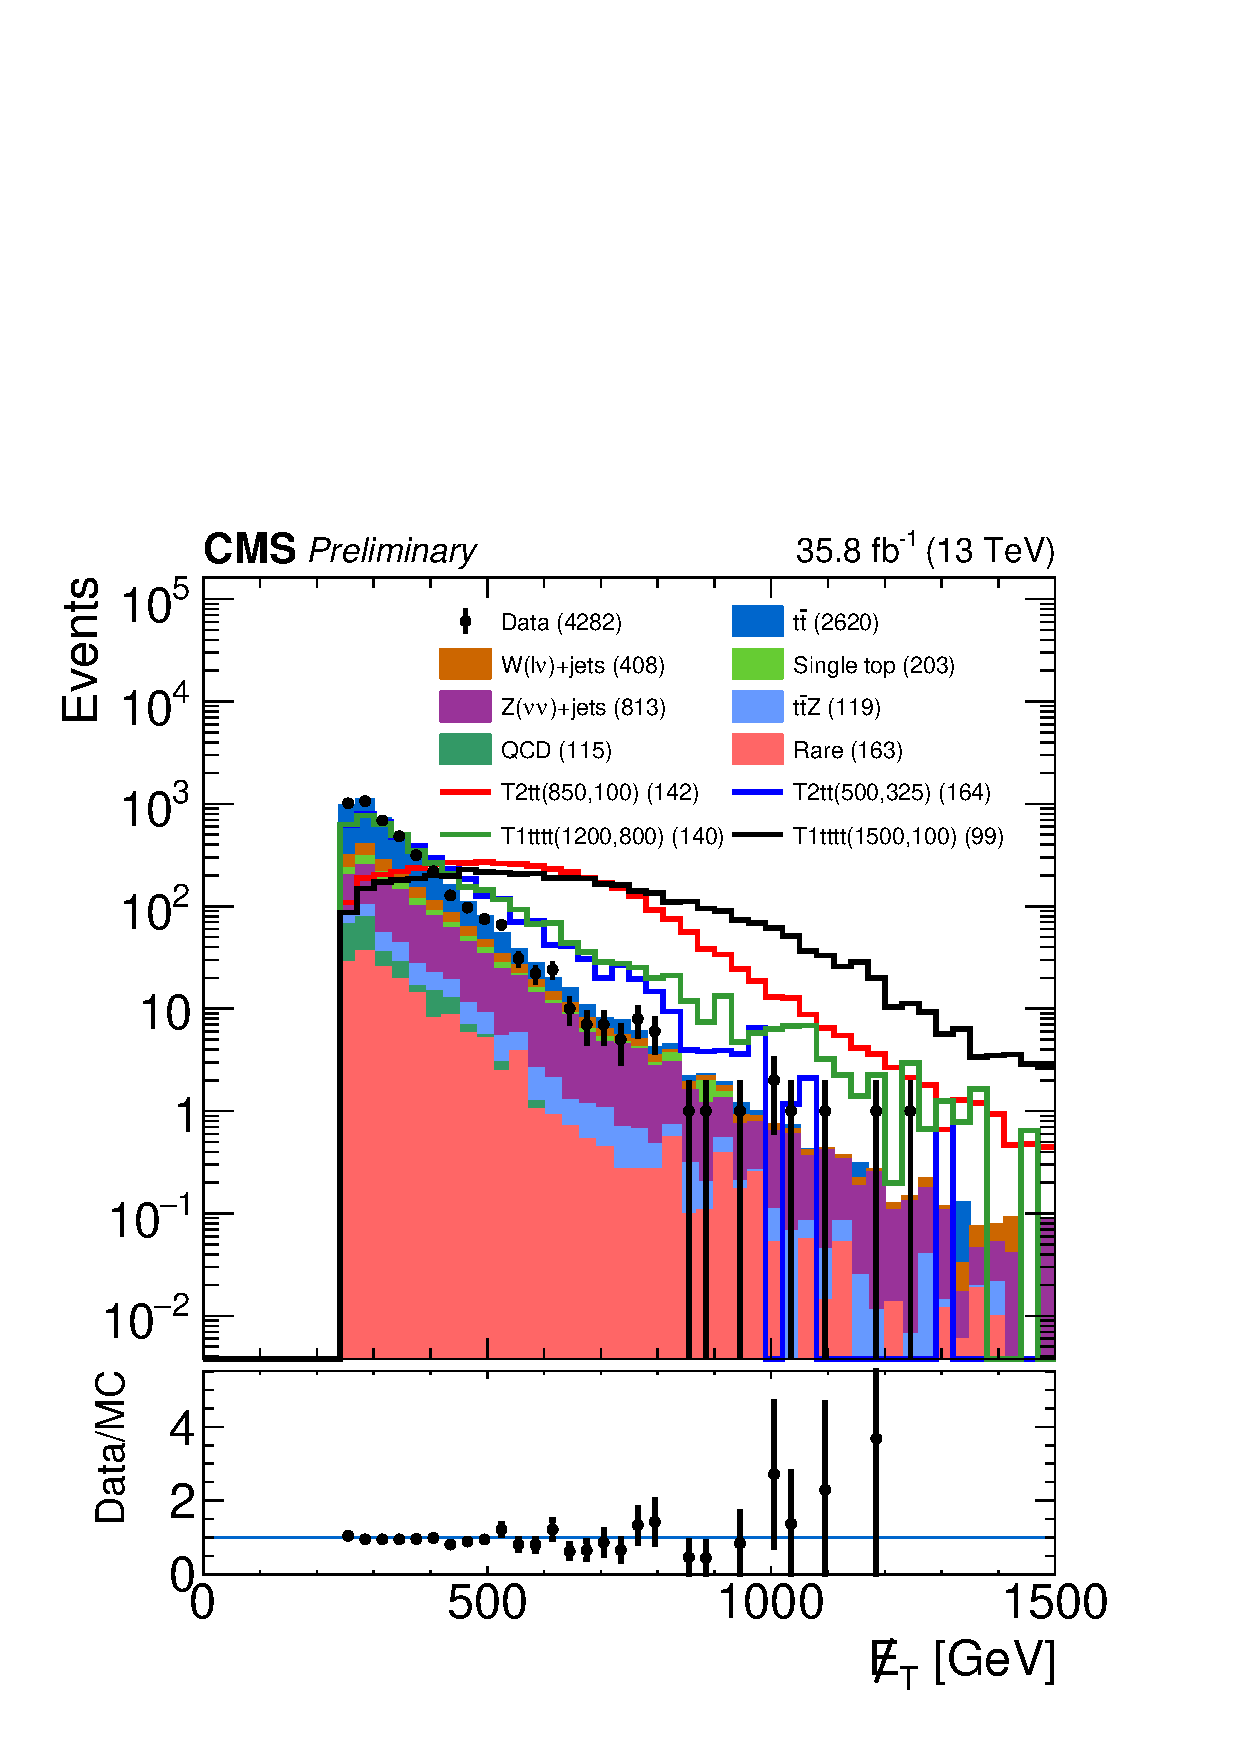
\includegraphics[width=0.45\linewidth]{sections/mc4/EvtSelSBOpt/figures/DataMC_MET_model_met_baseline.pdf}
    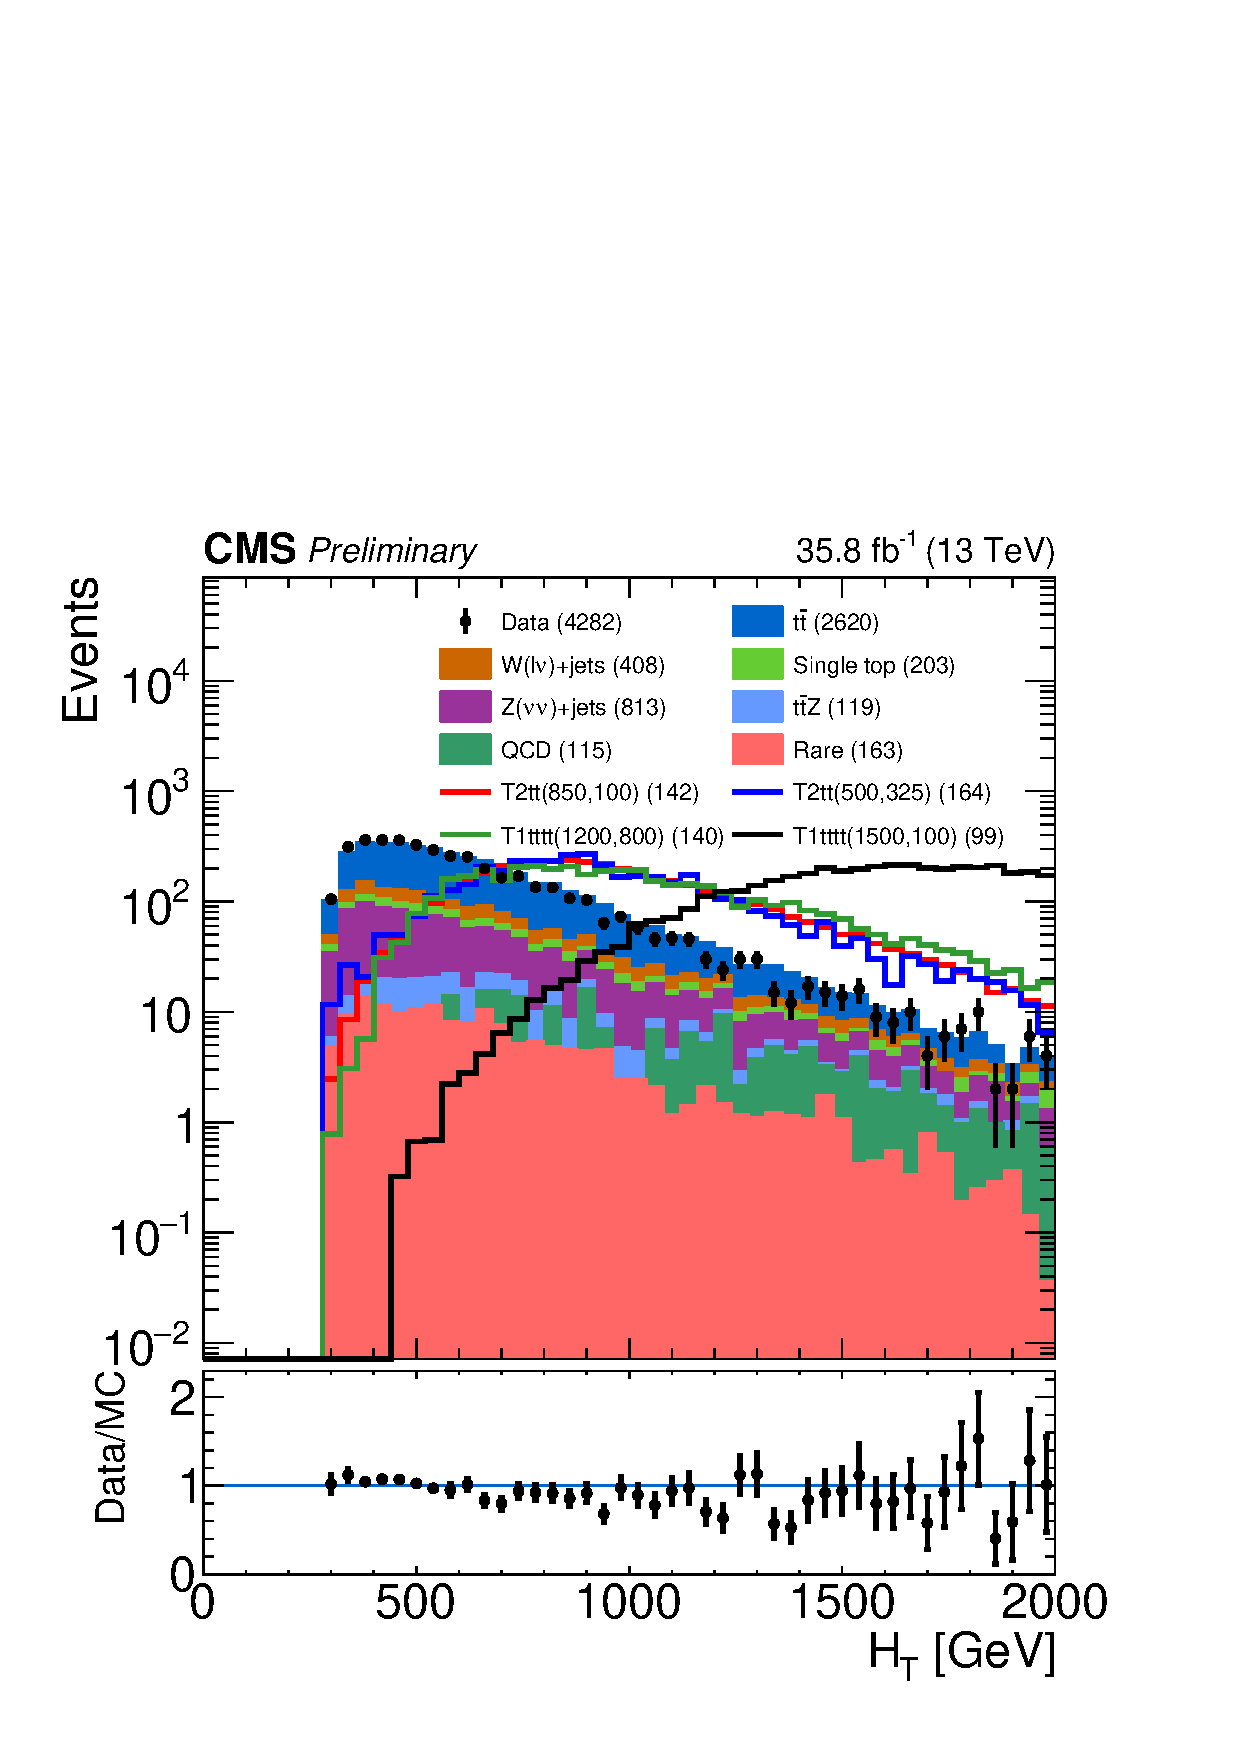
\includegraphics[width=0.45\linewidth]{sections/mc4/EvtSelSBOpt/figures/DataMC_MET_model_ht_baseline.pdf}\\
    \caption{Comparison of the distributions between total SM backgrounds from simulation and several signal points for \ntops, \nbjets, \MET and \MTTwo clock-wise with \HT at the bottom. Total SM backgrounds and signals are scaled to same data yield for a shape comparison. The yeilds for the Data and the SM backgrounds are in the legend.  The scale is included in the legend for the signal points. }
    \label{fig:compSBvars}
  \end{center}
\end{figure}

%Fig.~\ref{fig:compMT2vsMET} shows the 2D distributions of \MTTwo versus \MET for the major \ttbar background and two signals, i.e., T2tt(850, 100) and T2tt(500, 325). We can clearly see the shapes are different between the \ttbar background and the high stop mass signal point. For the low stop mass point, the correlation between \MTTwo and \MET is not as strong as the high mass point, however difference can still be seen between this signal and the \ttbar background.

%\begin{figure}[h]
%  \begin{center}
%    \includegraphics[width=0.32\linewidth]{}%eventSelection/figures/comb_TTbar_MT2_vs_met_baseline.pdf}
%    \includegraphics[width=0.32\linewidth]{}%eventSelection/figures/comb_Signal_T2tt_mStop850_mLSP100_MT2_vs_met_baseline.pdf}
%    \includegraphics[width=0.32\linewidth]{}%eventSelection/figures/comb_Signal_T2tt_mStop500_mLSP325_MT2_vs_met_baseline.pdf}
%    \caption{ 2D distributions of \MTTwo versus \MET for the major \ttbar background and two signal points, i.e., T2tt(850, 100) in the middle and T2tt(500, 325) in the right, after the baseline cuts. }
%    \label{fig:compMT2vsMET}
%  \end{center}
%\end{figure}

The search bins defined after baseline cuts (in total 84 bins) are illustrated in Fig.~\ref{fig:SBXX}. An improvement we make is switching from the \MTTwo variable to \HT variable for search bins where $\nbjets>=3$ or $\ntops>=3$ since these bins should be sensitive to the T1tttt signals where the \MTTwo cannot be clearly as defined with more than two reconstructed top quarks or provide the best sensitivity. 
To accommodate with increaing luminosity of 2016 data and improve our search sensitivity, we make harder search bins in
\MET, \HT and \MTTwo dimentions. The optimization was based on significance scan of each of \MET, \MTTwo and \HT dimentions. However
furthur adjustment was done to have reasonable control sample events for major background predictions.
The numbers displayed in the figures are the binning indices which are used throughout the analysis.
The bins with $\ntops>=3$ are important for T1tttt signal but for T2tt we do not use them for limit calculation.

\begin{figure}[h]
  \begin{center}
    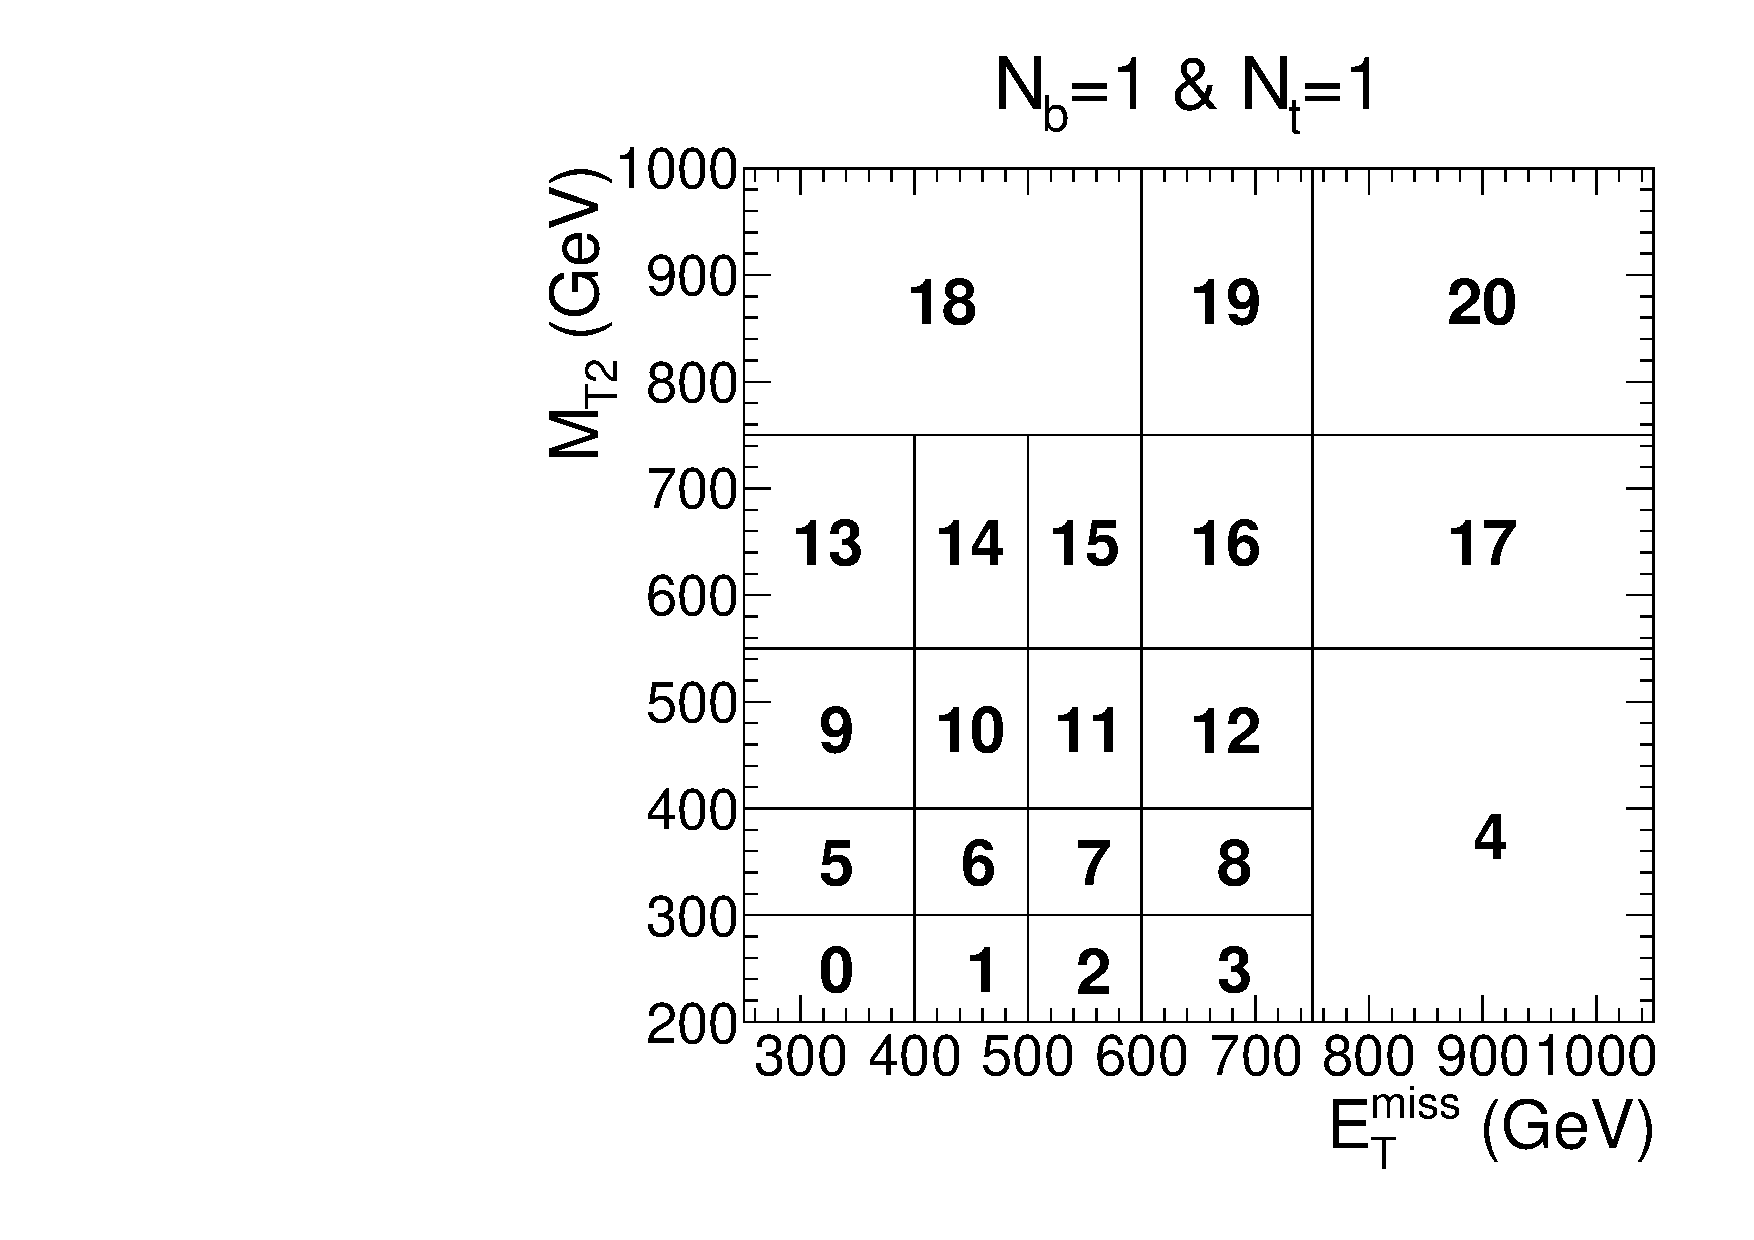
\includegraphics[width=0.30\linewidth]{sections/mc4/EvtSelSBOpt/figures/poly_MT2_vs_met_0.pdf}
    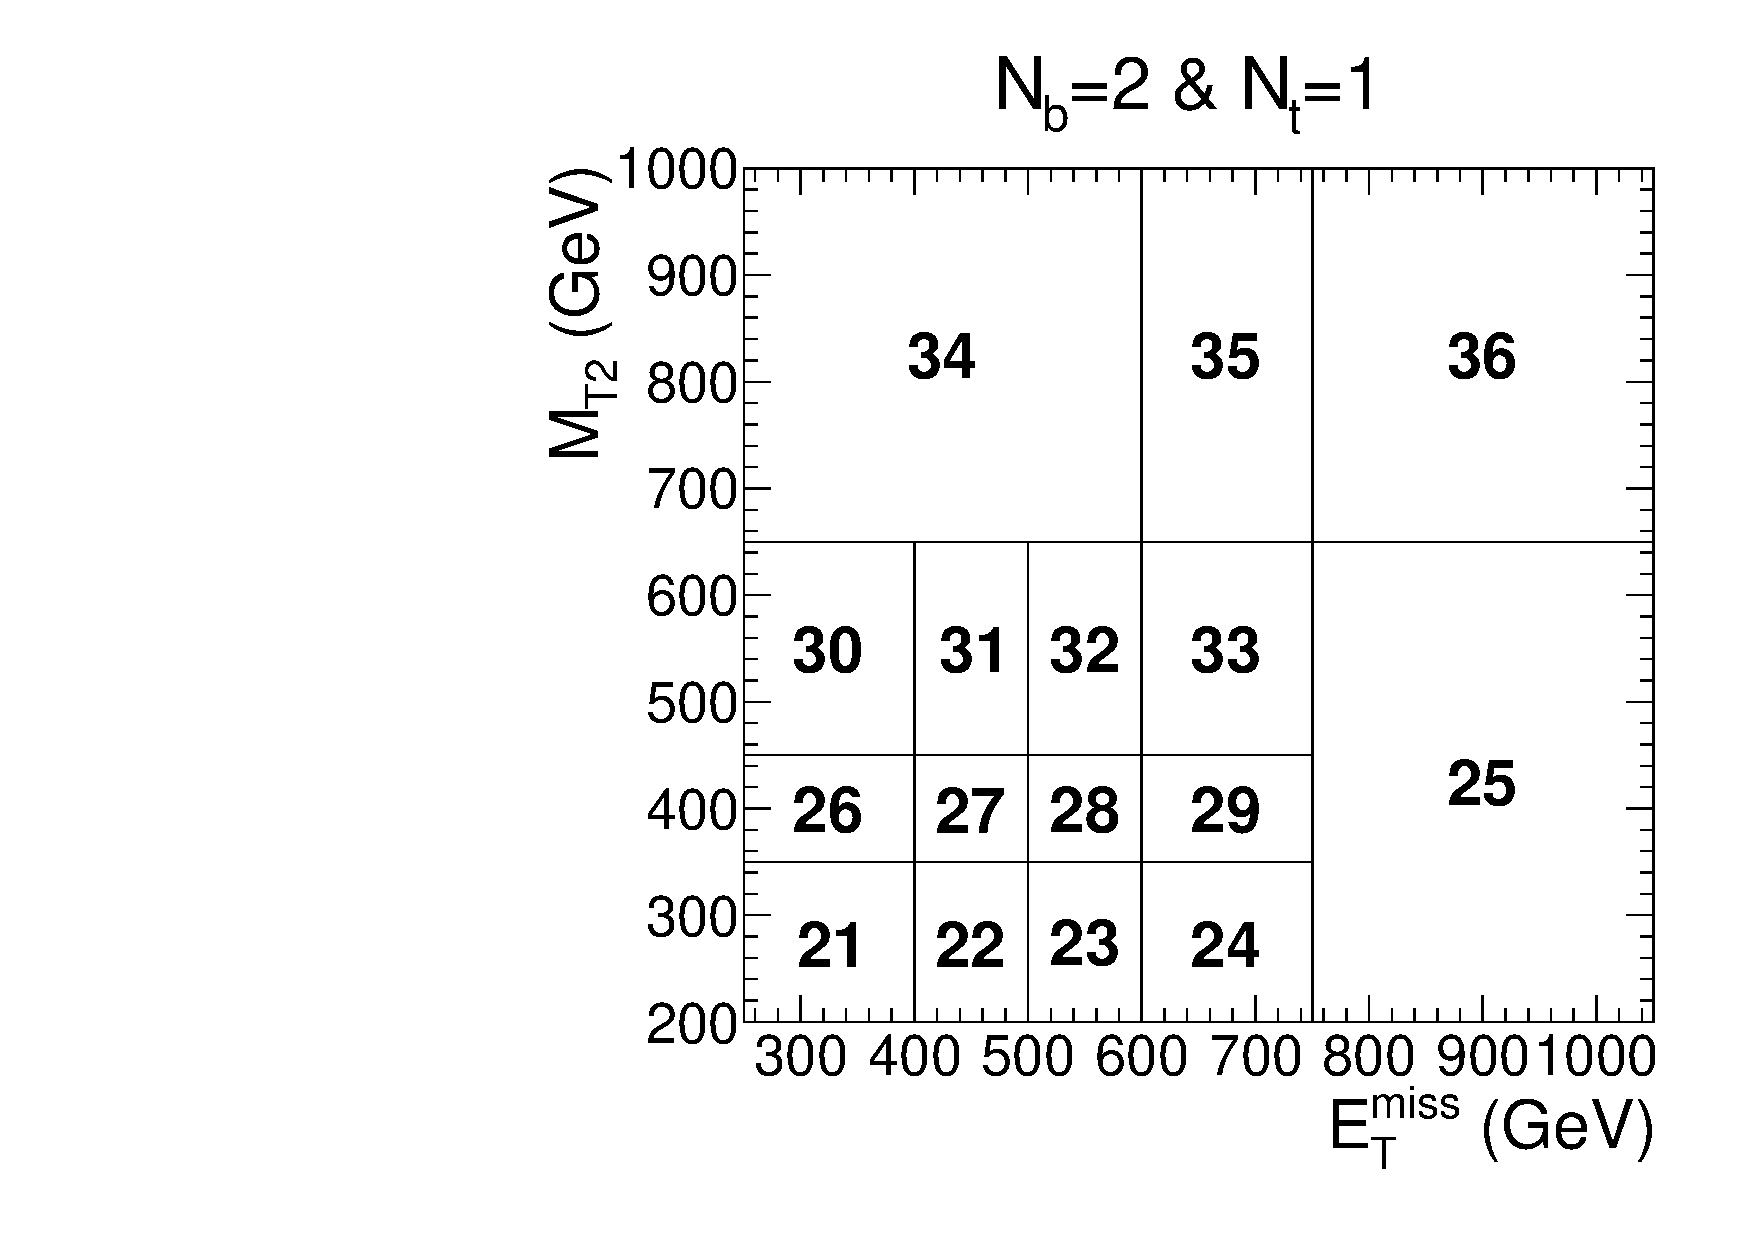
\includegraphics[width=0.30\linewidth]{sections/mc4/EvtSelSBOpt/figures/poly_MT2_vs_met_1.pdf}
    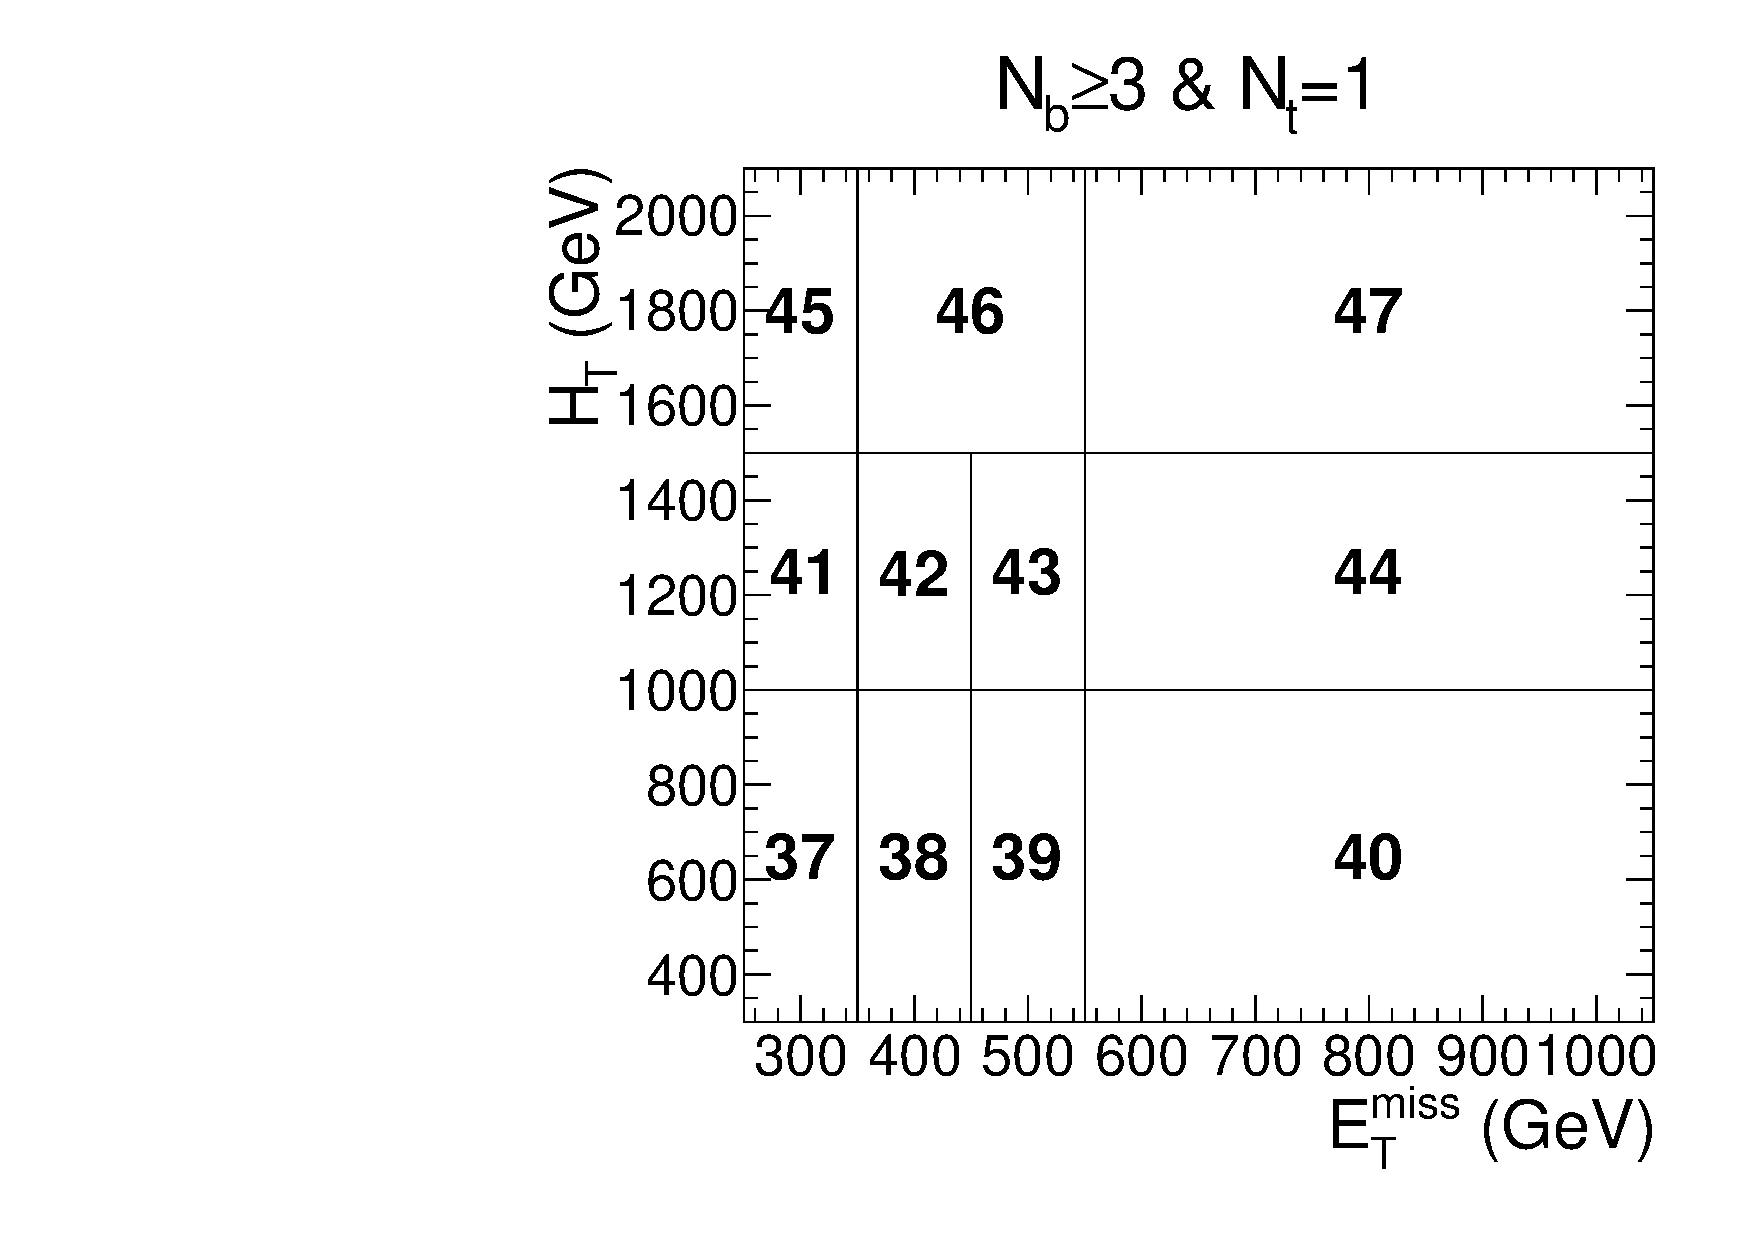
\includegraphics[width=0.30\linewidth]{sections/mc4/EvtSelSBOpt/figures/poly_MT2_vs_met_2.pdf} \\
    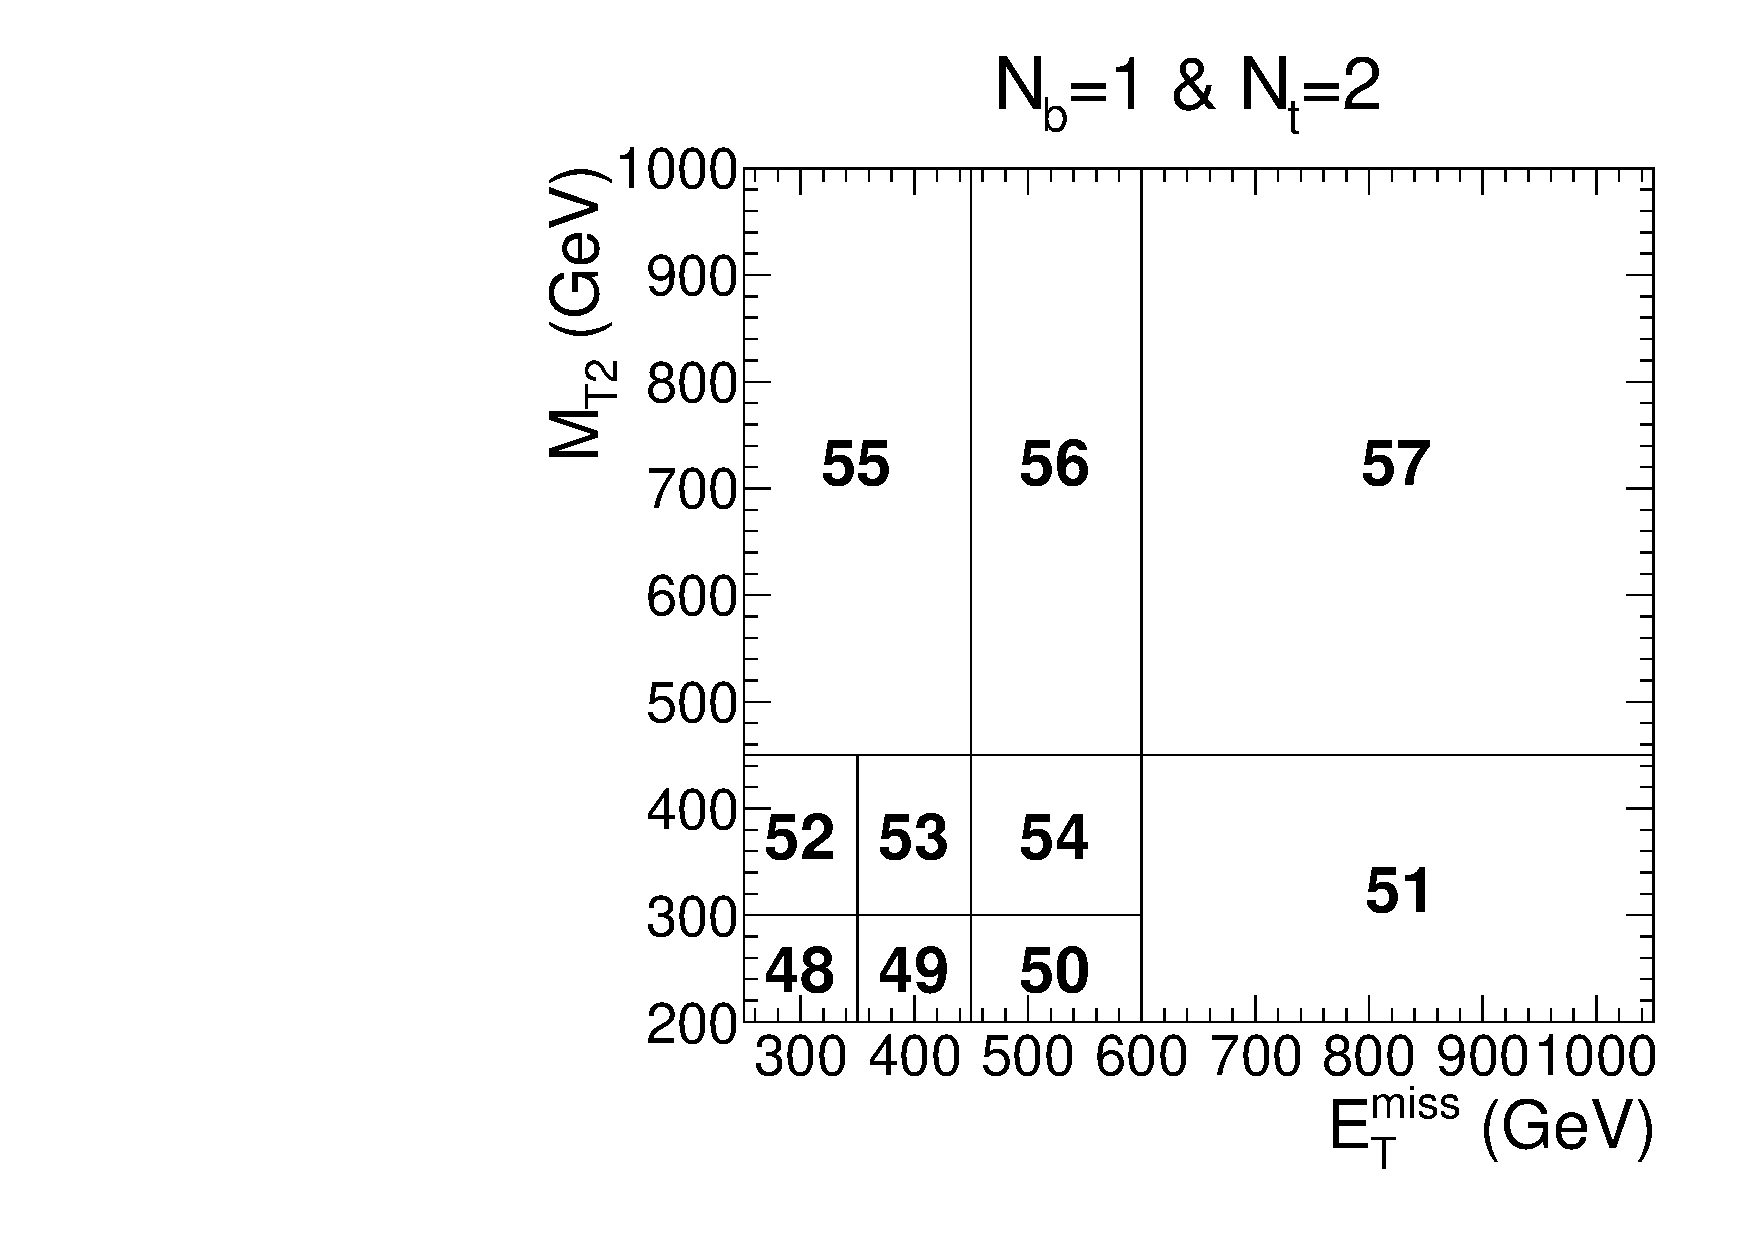
\includegraphics[width=0.30\linewidth]{sections/mc4/EvtSelSBOpt/figures/poly_MT2_vs_met_3.pdf} 
    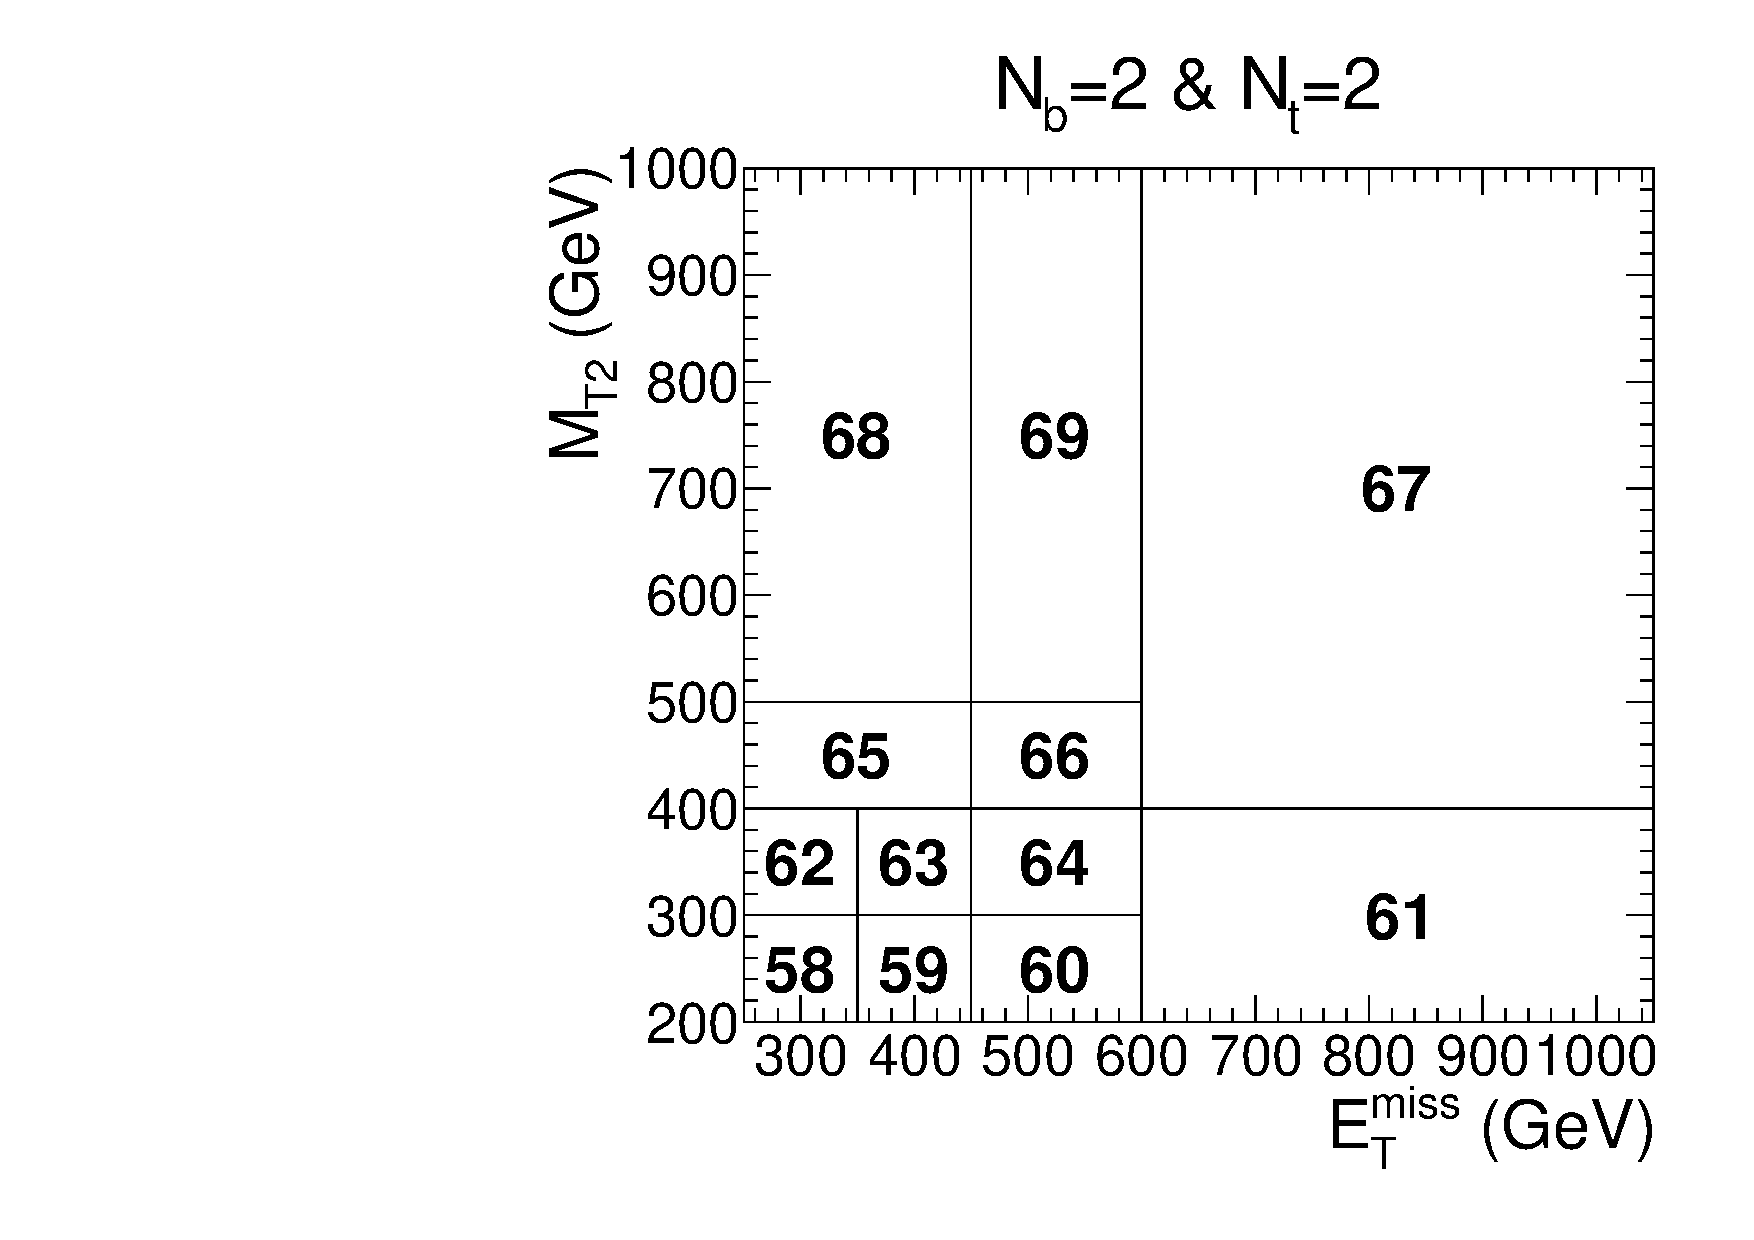
\includegraphics[width=0.30\linewidth]{sections/mc4/EvtSelSBOpt/figures/poly_MT2_vs_met_4.pdf} 
    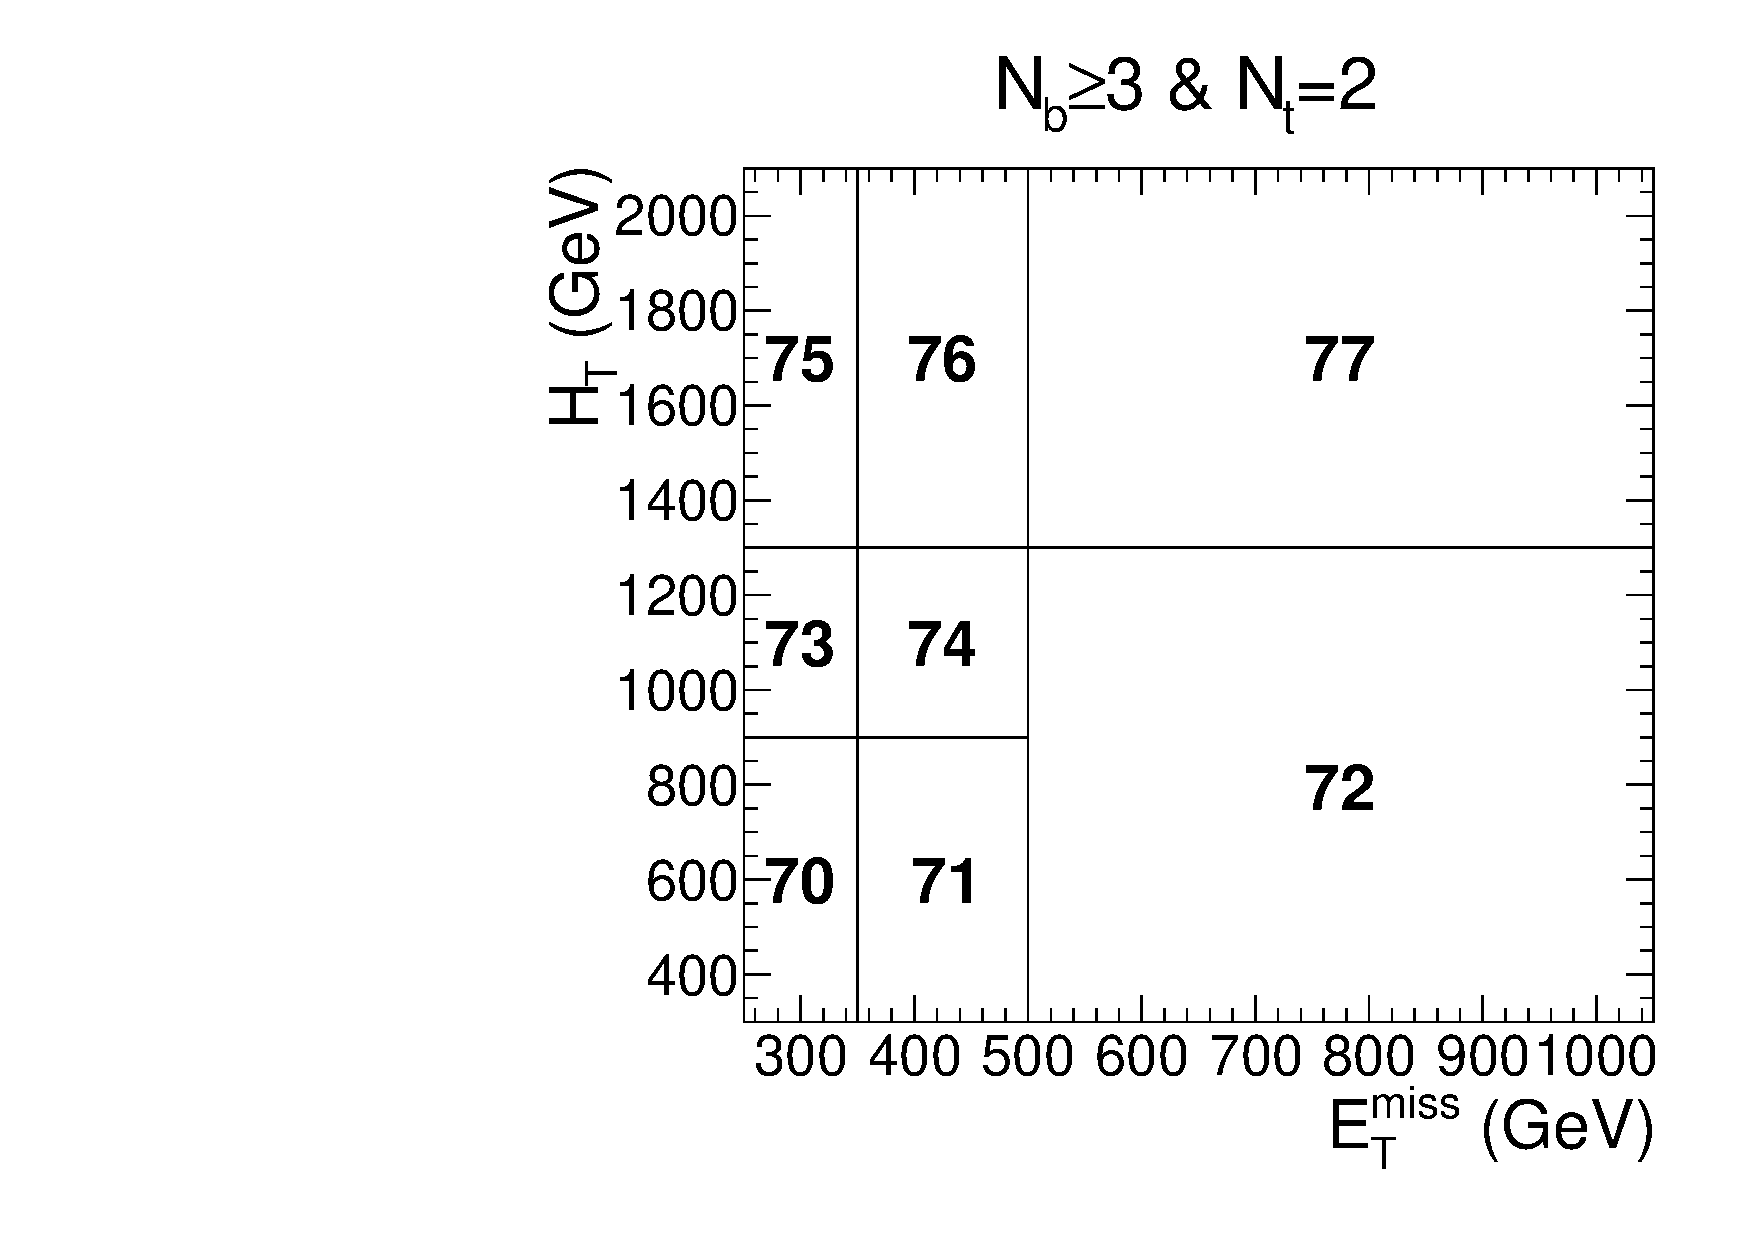
\includegraphics[width=0.30\linewidth]{sections/mc4/EvtSelSBOpt/figures/poly_MT2_vs_met_5.pdf} \\
    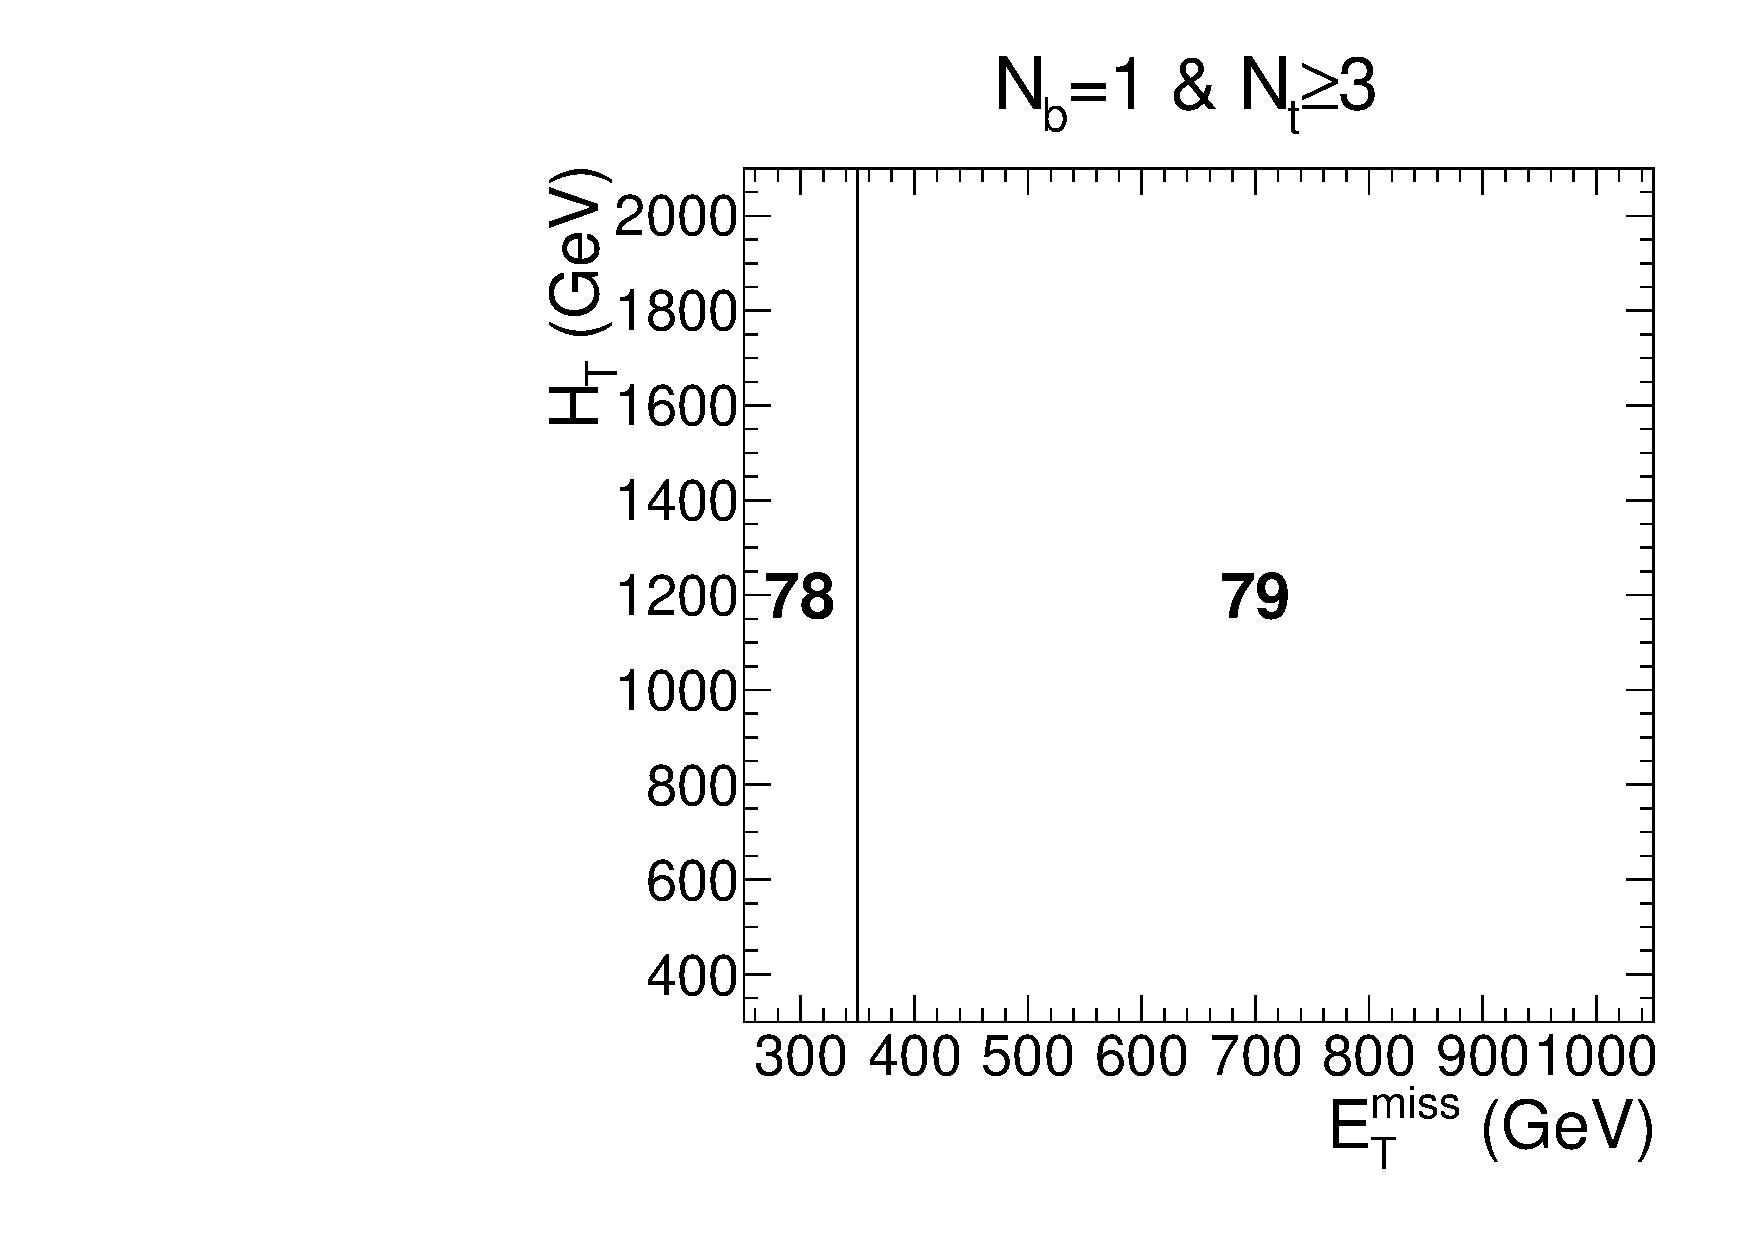
\includegraphics[width=0.30\linewidth]{sections/mc4/EvtSelSBOpt/figures/poly_MT2_vs_met_6.pdf} 
    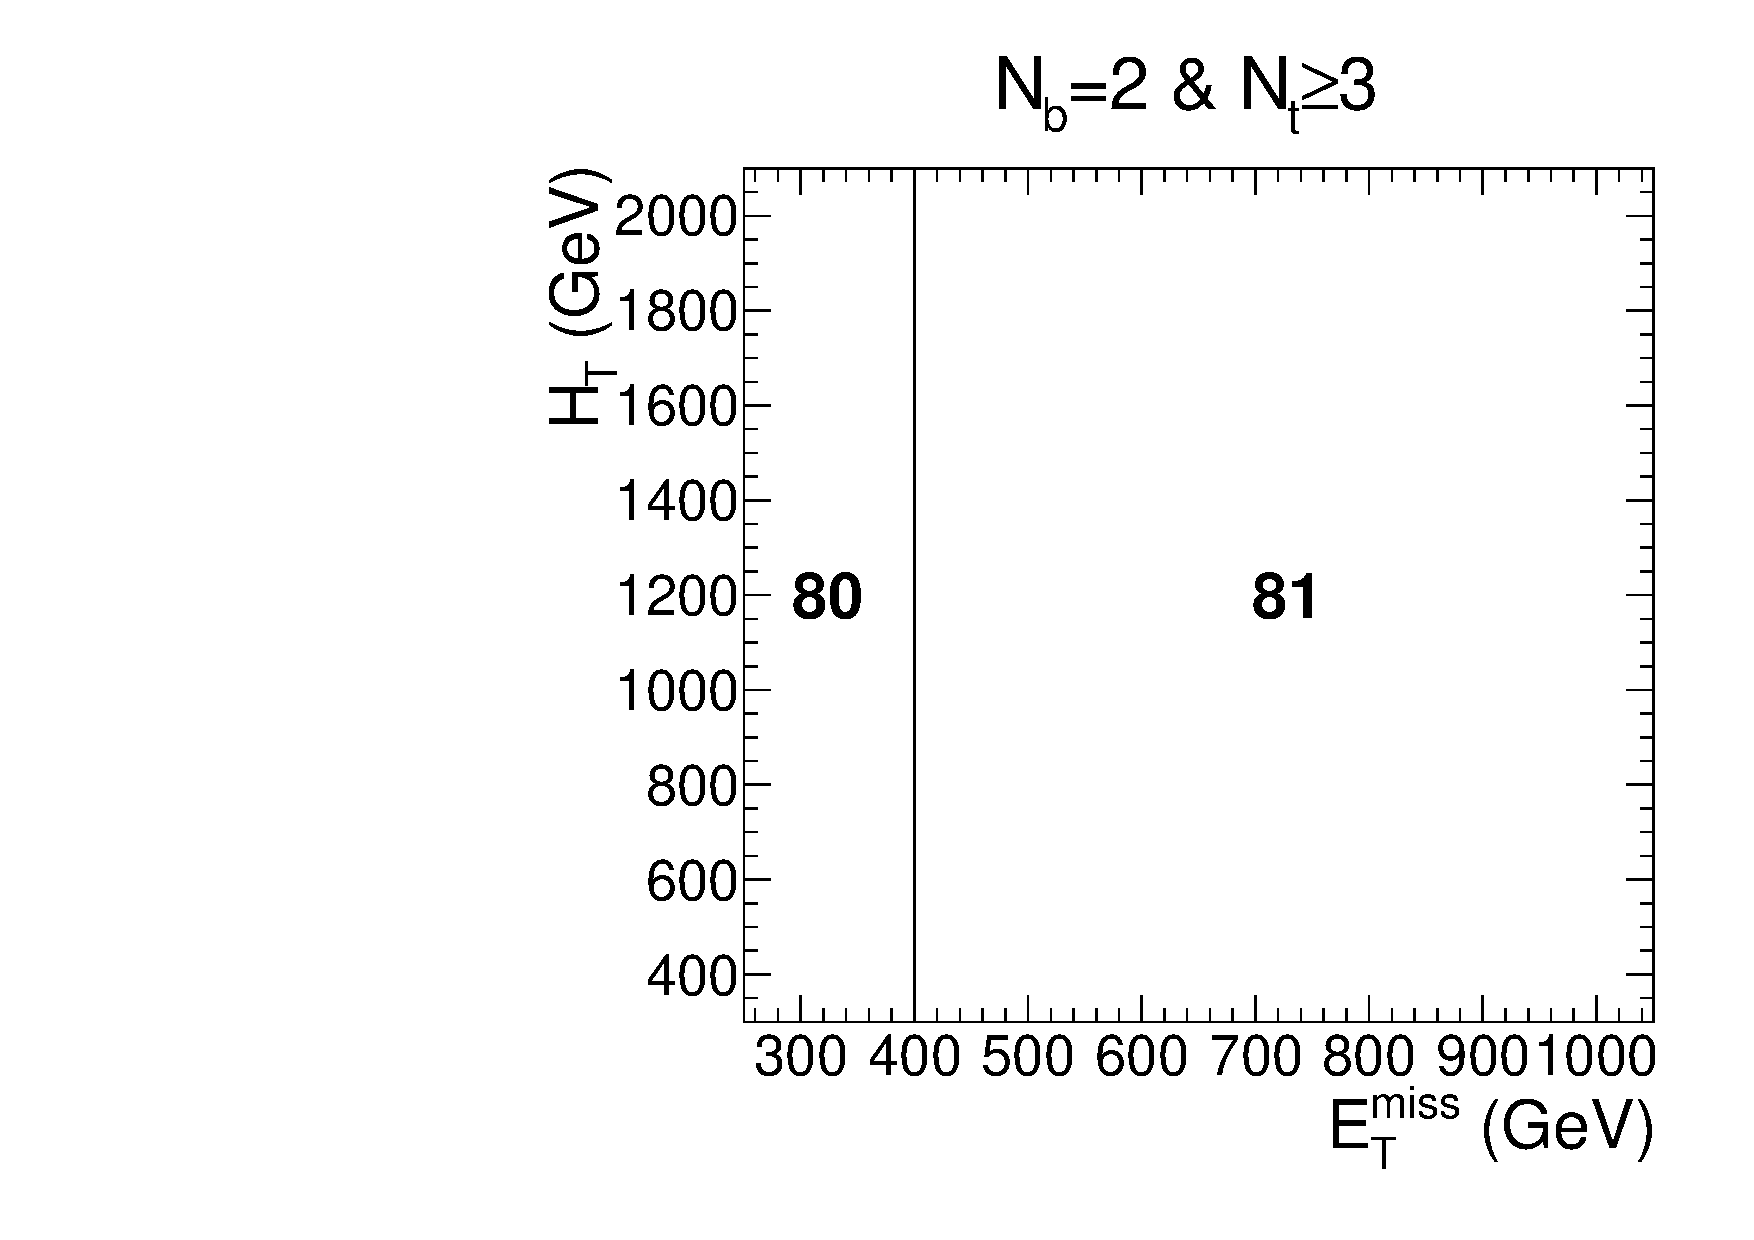
\includegraphics[width=0.30\linewidth]{sections/mc4/EvtSelSBOpt/figures/poly_MT2_vs_met_7.pdf} 
    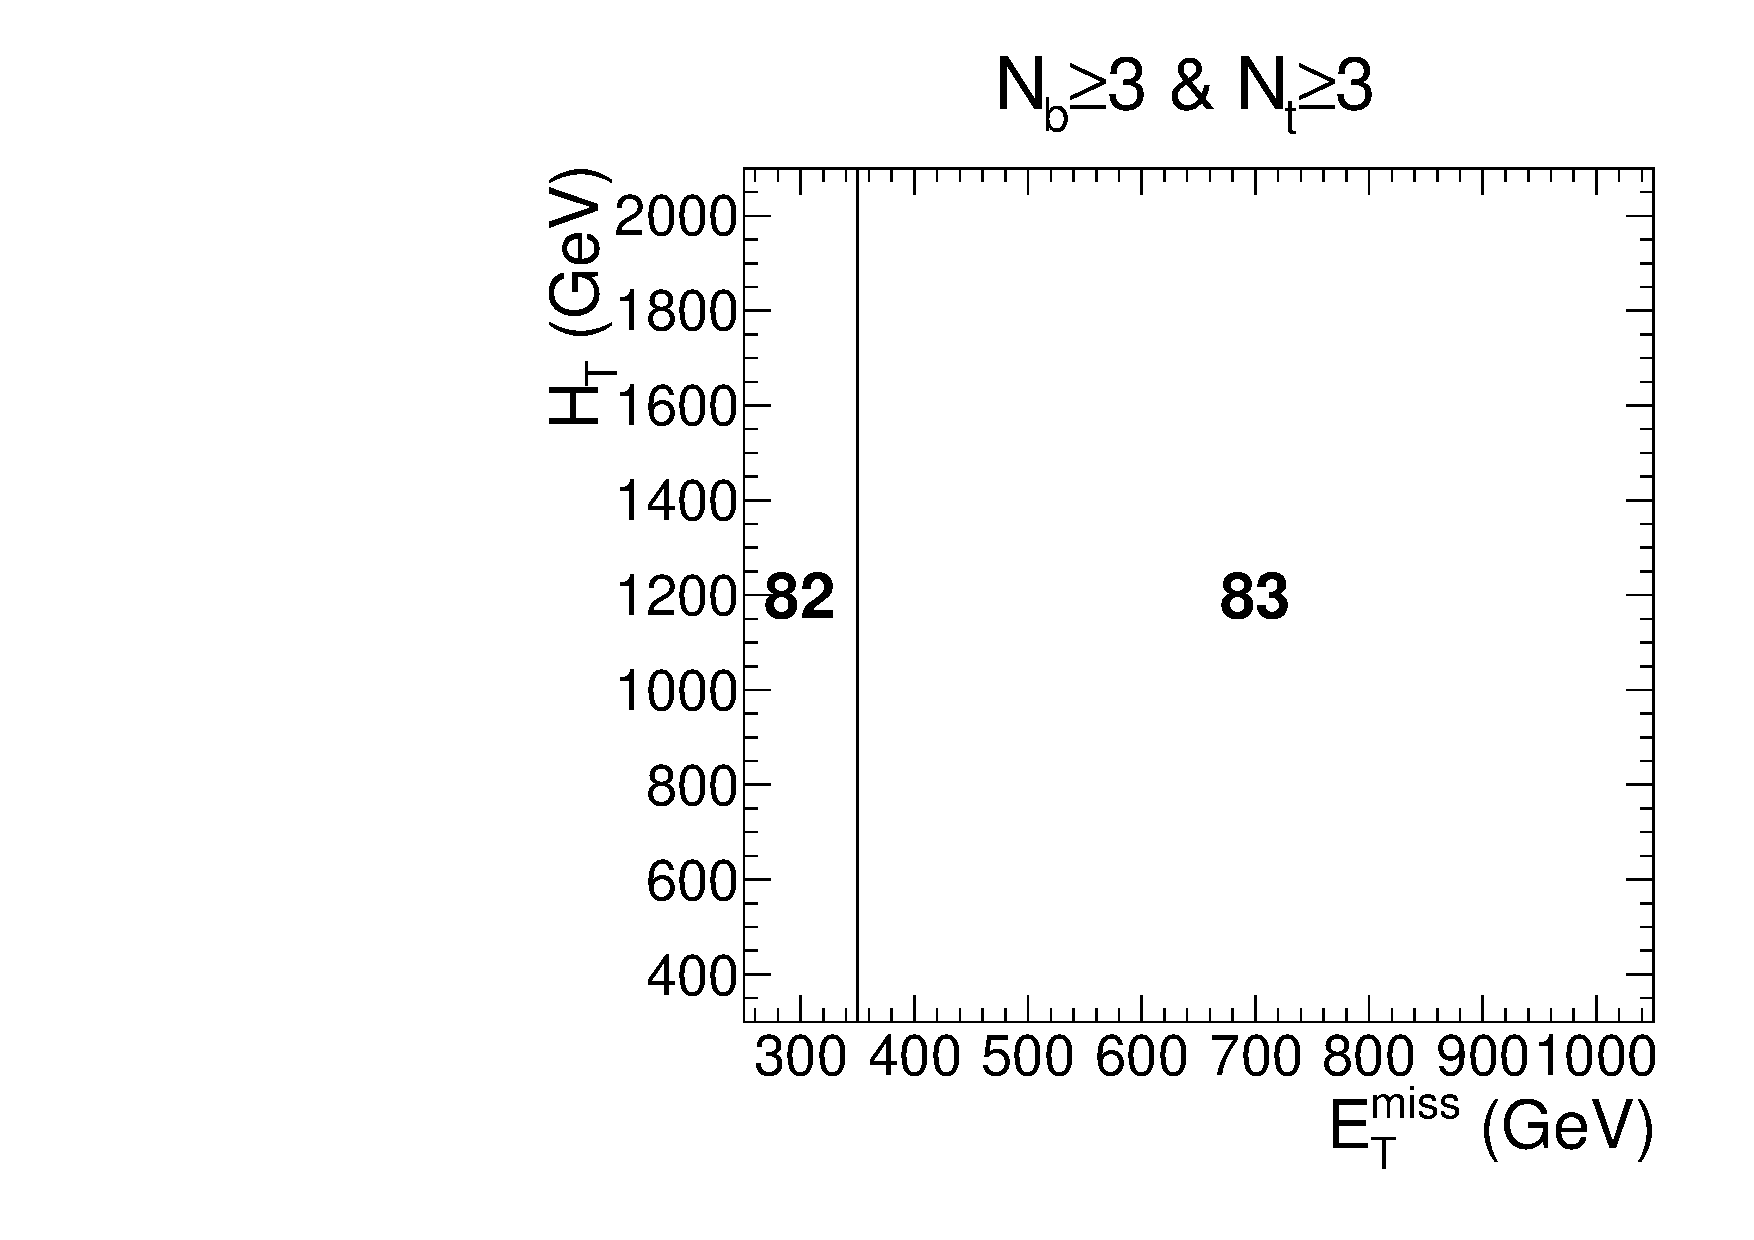
\includegraphics[width=0.30\linewidth]{sections/mc4/EvtSelSBOpt/figures/poly_MT2_vs_met_8.pdf} \\
    \caption{Original search bin definitions after baseline cuts (in total 84 search bins). }
    \label{fig:SBXX}
  \end{center}
\end{figure}

\subsection{MC samples for Background and Signal Studies}
\label{sec:sm-mc}

The analysis uses a set of Monte Carlo samples for background estimation method
development and predictions as well as SUSY signal samples for interpretation
of the results in the light of a number of simplified models. All the
background samples are generated with the Geant4-based CMS simulation 
application while all the signal samples for limit setting are generated
using the Fast Simulation application.

\paragraph{Standard Model Samples}

Monte Carlo samples of SM processes reconstructed with CMSSW release 8.0 
(Summer16) are used throughout this analysis note.
A complete list of these samples is shown in Tab.~\ref{tab:MCsamples}. 
The cross sections listed come from calculations performed at the 
next-to-next-to-leading-order (NNLO) unless otherwise noted.
All samples use the ``Moriond17" pileup scenario, which simulates a pileup 
distribution with an average of 25 interactions per bunch crossing and a 
25~ns interval between bunches.

% This table is out-dated, if needed, can copy the table from the MT2 AN2016_460
\begin{table}[hp]
\centering
\caption{Standard model Monte Carlo samples used in the analysis.}
\label{tab:MCsamples}
{\footnotesize
\begin{tabular}{lccc}
\hline \hline
Dataset & $\sigma$ (pb) & $\int$ (fb$^{-1}$) \\
\hline
\multicolumn{3}{c}{QCD MC samples (LO)} \\ \hline
QCD\_HT100to200\_TuneCUETP8M1\_13TeV-madgraphMLM-pythia8 & 27540000 & 0.01\\
QCD\_HT200to300\_TuneCUETP8M1\_13TeV-madgraphMLM-pythia8 & 1735000 & 0.01\\
QCD\_HT300to500\_TuneCUETP8M1\_13TeV-madgraphMLM-pythia8 & 366800 & 0.05\\
QCD\_HT500to700\_TuneCUETP8M1\_13TeV-madgraphMLM-pythia8 & 29370 & 0.67\\
QCD\_HT700to1000\_TuneCUETP8M1\_13TeV-madgraphMLM-pythia8 & 6524 & 2.30\\
QCD\_HT1000to1500\_TuneCUETP8M1\_13TeV-madgraphMLM-pythia8 & 1064 & 4.67\\
QCD\_HT1500to2000\_TuneCUETP8M1\_13TeV-madgraphMLM-pythia8 & 121.5 & 31.67\\
QCD\_HT2000toInf\_TuneCUETP8M1\_13TeV-madgraphMLM-pythia8 & 25.42 & 77.17\\
\hline
\multicolumn{3}{c}{SM \ttbar MC samples} \\ \hline
%TTJets\_TuneCUETP8M1\_13TeV-madgraphMLM-pythia8 & 816.0 & 13.90\\
TTJets\_SingleLeptFromT\_TuneCUETP8M1\_13TeV-madgraphMLM-pythia8 & 179.3 & 324.6\\
TTJets\_SingleLeptFromTbar\_TuneCUETP8M1\_13TeV-madgraphMLM-pythia8 & 179.3 & 335.7\\
TTJets\_DiLept\_TuneCUETP8M1\_13TeV-madgraphMLM-pythia8 & 86.66 & 351.2\\
TTJets\_HT-600to800\_TuneCUETP8M1\_13TeV-madgraphMLM-pythia8 & 2.615 & 1898\\
TTJets\_HT-800to1200\_TuneCUETP8M1\_13TeV-madgraphMLM-pythia8 & 1.077 & 3198\\
TTJets\_HT-1200to2500\_TuneCUETP8M1\_13TeV-madgraphMLM-pythia8 & 0.195 & 5063\\
TTJets\_HT-2500toInf\_TuneCUETP8M1\_13TeV-madgraphMLM-pythia8 & 0.002 & 218575\\
\hline
\multicolumn{3}{c}{SM \wlnu MC samples} \\ \hline
WJetsToLNu\_HT-100To200\_TuneCUETP8M1\_13TeV-madgraphMLM-pythia8 & 1635 & 6.20\\
WJetsToLNu\_HT-200To400\_TuneCUETP8M1\_13TeV-madgraphMLM-pythia8 & 437.0 & 11.97\\
WJetsToLNu\_HT-400To600\_TuneCUETP8M1\_13TeV-madgraphMLM-pythia8 & 59.50 & 31.96\\
WJetsToLNu\_HT-600ToInf\_TuneCUETP8M1\_13TeV-madgraphMLM-pythia8 & 22.80 & 45.44\\
WJetsToLNu\_HT-600To800\_TuneCUETP8M1\_13TeV-madgraphMLM-pythia8 & 15.50 & 257.1\\
WJetsToLNu\_HT-800To1200\_TuneCUETP8M1\_13TeV-madgraphMLM-pythia8 & 6.366 & 247.4\\
WJetsToLNu\_HT-1200To2500\_TuneCUETP8M1\_13TeV-madgraphMLM-pythia8 & 1.614 & 158.4\\
WJetsToLNu\_HT-2500ToInf\_TuneCUETP8M1\_13TeV-madgraphMLM-pythia8 & 0.037 & 6770\\
\hline
\multicolumn{3}{c}{SM \znunu MC samples} \\ \hline
ZJetsToNuNu\_HT-100To200\_13TeV-madgraph & 345.0 & 14.92\\
ZJetsToNuNu\_HT-200To400\_13TeV-madgraph & 96.38 & 52.22\\
ZJetsToNuNu\_HT-400To600\_13TeV-madgraph & 13.46 & 75.34\\
ZJetsToNuNu\_HT-600ToInf\_13TeV-madgraph & 5.170 & 196.5\\
ZJetsToNuNu\_HT-600To800\_13TeV-madgraph & 3.146 & 75.34\\
ZJetsToNuNu\_HT-800To1200\_13TeV-madgraph & 1.453 & 75.34\\
ZJetsToNuNu\_HT-1200To2500\_13TeV-madgraph & 0.359 & 75.34\\
ZJetsToNuNu\_HT-2500ToInf\_13TeV-madgraph & 0.008487& 75.34\\
\hline
\multicolumn{3}{c}{SM \zll MC samples} \\ \hline
DYJetsToLL\_M-50\_TuneCUETP8M1\_13TeV-madgraphMLM-pythia8 & 6025 & 1.50\\
DYJetsToLL\_M-50\_HT-100to200\_TuneCUETP8M1\_13TeV-madgraphMLM-pythia8 & 171.5 & 15.31\\
DYJetsToLL\_M-50\_HT-200to400\_TuneCUETP8M1\_13TeV-madgraphMLM-pythia8 & 52.58 & 18.18\\
DYJetsToLL\_M-50\_HT-400to600\_TuneCUETP8M1\_13TeV-madgraphMLM-pythia8 & 6.984 & 155.0\\
DYJetsToLL\_M-50\_HT-600to800\_TuneCUETP8M1\_13TeV-madgraphMLM-pythia8 & 1.676 & xxx\\
DYJetsToLL\_M-50\_HT-800to1200\_TuneCUETP8M1\_13TeV-madgraphMLM-pythia8 & 0.831 & xxx\\
DYJetsToLL\_M-50\_HT-1200to2500\_TuneCUETP8M1\_13TeV-madgraphMLM-pythia8 & 0.143 & xxx\\
DYJetsToLL\_M-50\_HT-2500toInf\_TuneCUETP8M1\_13TeV-madgraphMLM-pythia8 & 0.00319 & xxx\\
\hline
\multicolumn{3}{c}{SM single-top MC samples} \\ \hline
%ST\_s-channel\_4f\_leptonDecays\_13TeV-amcatnlo-pythia8\_TuneCUETP8M1 & 3.340 & 183.6\\
%ST\_t-channel\_antitop\_4f\_leptonDecays\_13TeV-powheg-pythia8\_TuneCUETP8M1 & 26.23 & 64.64\\
%ST\_t-channel\_top\_4f\_leptonDecays\_13TeV-powheg-pythia8\_TuneCUETP8M1 & 44.07 & 74.88\\
ST\_tW\_antitop\_5f\_inclusiveDecays\_13TeV-powheg-pythia8\_TuneCUETP8M1 & 35.80 (NLO) & 27.93\\
ST\_tW\_top\_5f\_inclusiveDecays\_13TeV-powheg-pythia8\_TuneCUETP8M1 & 35.80 (NLO) & 27.81\\
\hline
\multicolumn{3}{c}{SM diboson and other rare process MC samples} \\ \hline
ttHJetTobb\_M125\_13TeV\_amcatnloFXFX\_madspin\_pythia8 & 0.293 & 18269\\
TTZToLLNuNu\_M-10\_TuneCUETP8M1\_13TeV-amcatnlo-pythia8 & 0.228 & 811.4\\
TTZToQQ\_TuneCUETP8M1\_13TeV-amcatnlo-pythia8 & 0.530 & 663.4\\
TTWJetsToLNu\_TuneCUETP8M1\_13TeV-amcatnloFXFX-madspin-pythia8 & 0.204 & 635.6\\
TTWJetsToQQ\_TuneCUETP8M1\_13TeV-amcatnloFXFX-madspin-pythia8 & 0.423 & 1018\\
%ZH\_HToBB\_ZToNuNu\_M125\_13TeV\_amcatnloFXFX\_madspin\_pythia8 & 0.100 & 12116\\
%WH\_HToBB\_WToLNu\_M125\_13TeV\_amcatnloFXFX\_madspin\_pythia8 & 0.260 & 4782\\
WW\_TuneCUETP8M1\_13TeV\_pythia8 & 115.0 & 64.26\\
WZ\_TuneCUETP8M1\_13TeV\_pythia8 & 47.13 & 1339\\
ZZ\_TuneCUETP8M1\_13TeV\_pythia8 & 16.523 & 5556\\
%TTTT\_TuneCUETP8M1\_13TeV-amcatnlo-pythia8 & 0.009 & 57031\\
WWZ\_TuneCUETP8M1\_13TeV-amcatnlo-pythia8 & 0.165 & 1341\\
WZZ\_TuneCUETP8M1\_13TeV-amcatnlo-pythia8 & 0.056 & 3938\\
ZZZ\_TuneCUETP8M1\_13TeV-amcatnlo-pythia8 & 0.014 & 15297\\
\hline \hline
\end{tabular}
}
\end{table}

\paragraph{Signal samples}

Diagrams associated with the signal simplified models (SMS) used in this search for interpretation of the results are shown in Fig~\ref{Fig:signal_diagrams}. The top diagram is often referred to as T2tt($x,y$) and represents direct squark-antisquark pair production with $x$ and $y$ the top squark and \chiOneZero masses, respectively~\cite{CMS-SMS-paper}. Under the assumption that the SUSY particles that could decay to top squarks are too heavy and beyond the reach of LHC Run 2, this diagram would represent the dominant process for top squark pair production and the target signal process for this analysis.

If the gluino is within the LHC reach in Run 2, gluino-induced processes such as those in the bottom row of Fig~\ref{Fig:signal_diagrams} would become relevant to the analysis. The bottom left diagram is called T1tttt($x,y$) with $x$ and $y$ the gluino and \chiOneZero masses.
In this model, the gluino undergoes a three-body decay into \ensuremath{\rm t}, \ensuremath{\rm \bar{t}} and 
\chiOneZero. The event kinematics are similar to the case
where
$\gluino\to\mathrm{t}\sTop, \sTop\to\mathrm{t}\chiOneZero$~\cite{CMS-SMS-paper}
as in the other model shown on the bottom right, denoted as 
T5ttcc($x,y,z$).
The numbers in parentheses refer to the gluino, top squark, and 
\chiOneZero masses. 

Cross sections for a couple of mass points are shown in 
Tab.~\ref{tab:signalMC} for the T2tt and T1tttt SMS. 
These selected points were generated with full simulation and were used for
cut flow studies and search region optimization. Limit setting was performed
using fast simulation signal samples.

%%T2tt mass points selected for the study, with motivation. T1tttt and the dark matter signal points used for 
%%additional studies aiming for next stage of work.

\begin{table}[hp]
\centering
\caption{Cross sections for a couple of mass points for the T2tt and T1tttt 
Simplified Models. The selected points were generated with full simulation.} %Note that all samples are generated with FullSim.}
\label{tab:signalMC}
{\footnotesize
\begin{tabular}{lccc}
\hline \hline
Dataset & $\sigma$ (pb) & $\int$ (fb$^{-1}$) \\
\hline
SMS-T2tt\_mStop-500\_mLSP-325\_TuneCUETP8M1\_13TeV-madgraph-pythia8 & 0.51848 & 748 \\
SMS-T2tt\_mStop-850\_mLSP-100\_TuneCUETP8M1\_13TeV-madgraphMLM-pythia8 & 0.01896 & 12694 \\
\hline
SMS-T1tttt\_mGluino-1500\_mLSP-100\_TuneCUETP8M1\_13TeV-madgraph-pythia8 & 0.014 & 7268\\
SMS-T1tttt\_mGluino-1200\_mLSP-800\_TuneCUETP8M1\_13TeV-madgraph-pythia8 & 0.086 & 1719 \\
%T5ttttDeg\_mGo1300\_mStop300\_mCh285\_mChi280\_23bodydec\_v2 (private) & 0.0460525 & 951 \\
%T5ttttDeg\_mGo1300\_mStop300\_mChi280\_4bodydec\_v2 (private) & 0.0460525 & 956 \\ 
%TTDMDMJets\_M600GeV\_Tune4C\_13TeV-madgraph-tauola & 0.1038 & 1219 \\
%TTDMDMJets\_M1000GeV\_Tune4C\_13TeV-madgraph-tauola & 0.01585 & 7686 \\
\hline \hline
\end{tabular}
\footnotesize}
\end{table}



\clearpage
\section{Background estimation}

The standard model processes are suppressed after the baseline selection criteria are applied, and signal sensitivities are optimized through the search bin design. However, there are still irreducible standard model backgrounds in the search region. In this analysis, the events from \ttbar, $W$+jets and single top are the major background. $Z$+jets, QCD and other rare processes also make non-negligible contributions in some search bins. The simulated background distributions are shown in the Fig~\ref{fig:c4bgmcpie} in the \ntops and \nbjets categories.

\begin{figure}[htbp]
 \begin{center}
  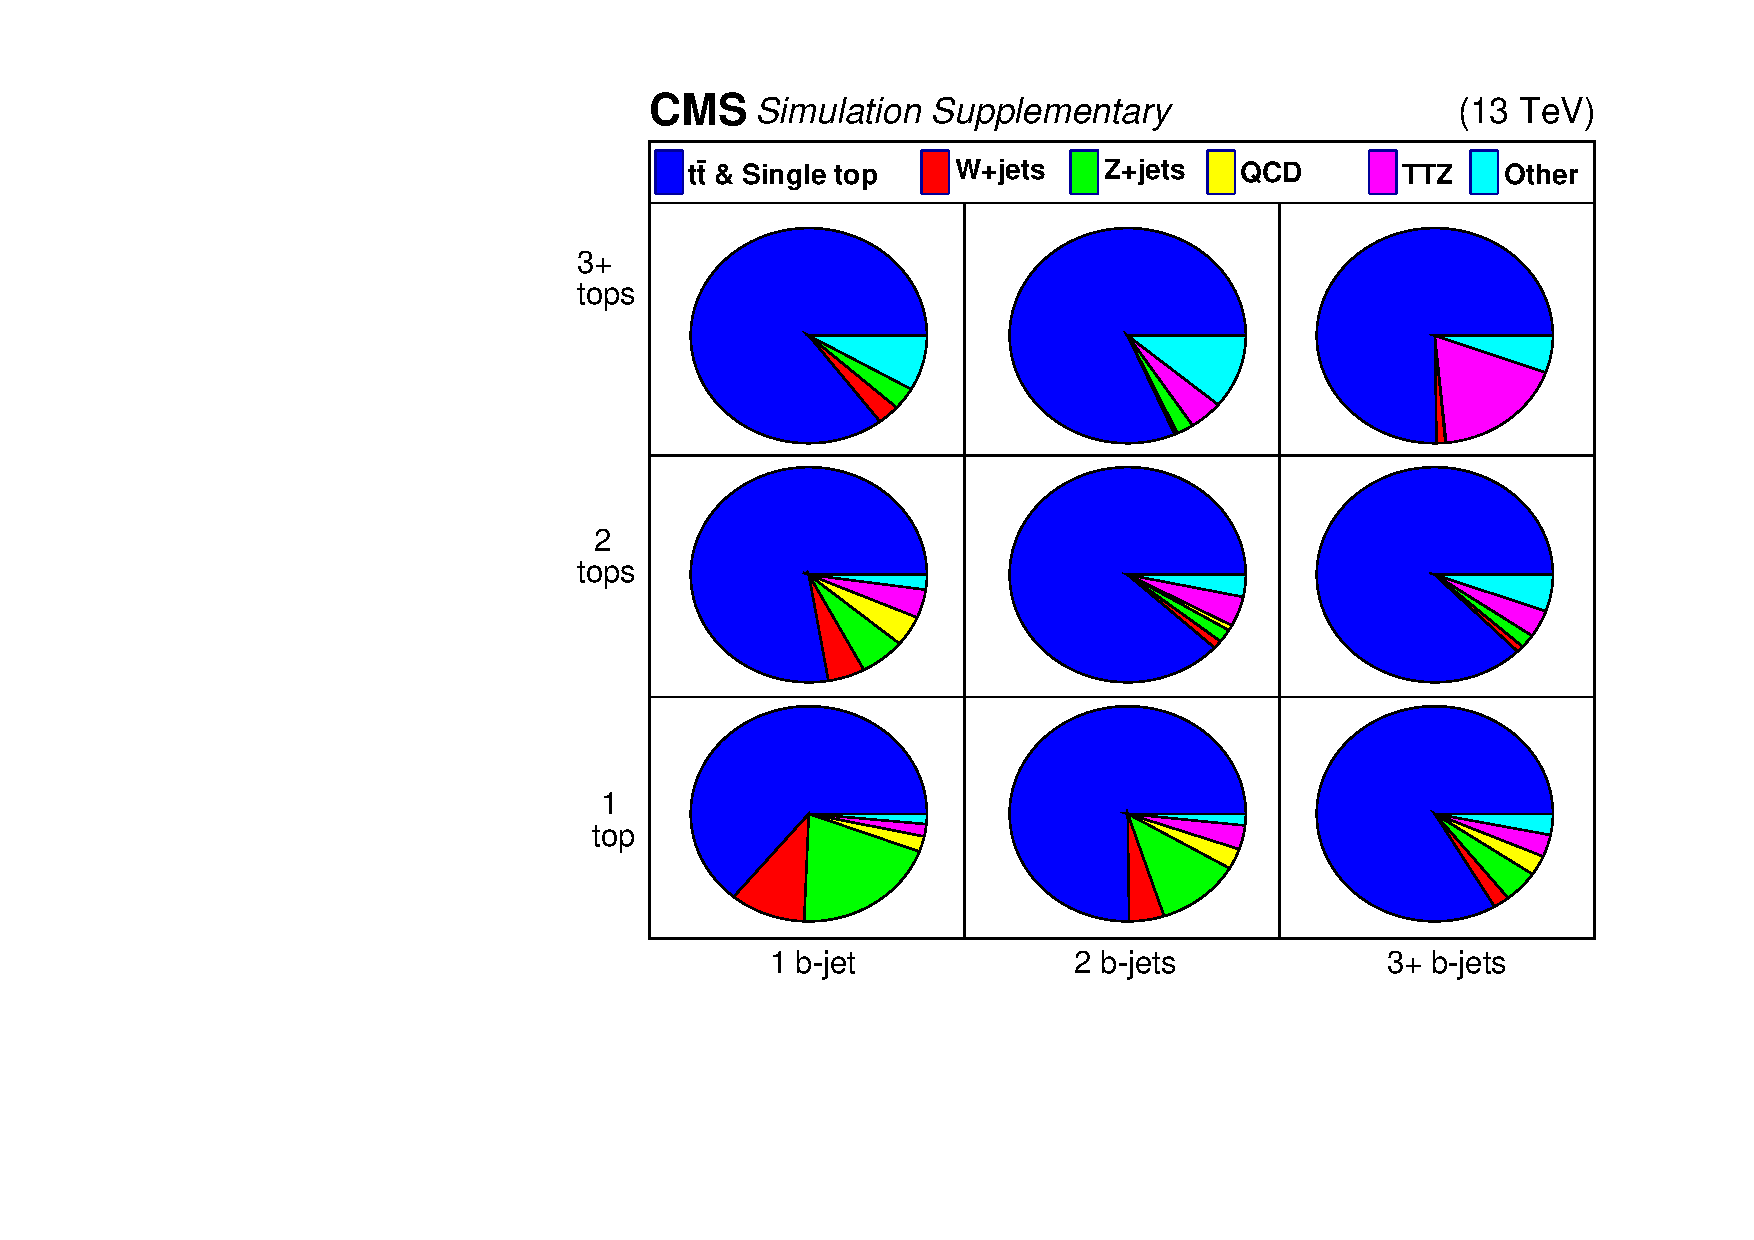
\includegraphics[width=0.85\textwidth]{figures/c4/c4_bg_mcpie.pdf}
 \end{center}
 \caption{Background pie chart, from simulation}
 \label{fig:c4bgmcpie}
\end{figure}

\clearpage
\subsection{Backgrounds from top and W decays}
The background from \ttbar, $W$+jets and single-top events that is not removed by the explicit lepton-veto and isolated track veto is the largest background in the analysis. It can contain either a hadronically decaying tau lepton or light leptons (electrons or muons) that are not isolated, not identified/reconstructed or are out of the acceptance region. Both types of background are estimated using the "translation factor method" (described in this section). The classic lost lepton method, which is used to predict specifically the events with light leptons, will be discussed in the following section. It serves as an important cross-check to the translation factor method.

\clearpage
\subsubsection{Translation factor method}
\label{sec:c4bgtf}
The translation factor is the ratio between the signal region yield and single lepton control sample yield in the simulation samples (\ttbar, $W$+jets and single top). The translation factor method is straightforward to apply. First, we calculate the translation factors for each search bin in the single lepton control sample in simulation events. The simulation events are corrected to account for residual differences with respect to data with ISR-reweighting, b-jet tag efficiencies and lepton reconstruction efficiencies. Then, we apply those factors to the single lepton control samples in data to estimate the backgrounds. The translation factors for misidentified leptons (lost lepton) and decaying tau leptons are shown in Figs~\ref{fig:hadtau_TF} and \ref{fig:lostle_TF}, for the single muon and electron control samples respectively. The final prediction combines the results from the single electron and single muon samples together (Figs~\ref{fig:TAUpredictionSB} and \ref{fig:LLpredictionSB}). 

\begin{figure}[htbp]
  \begin{center}
  \begin{tabular}{c}
  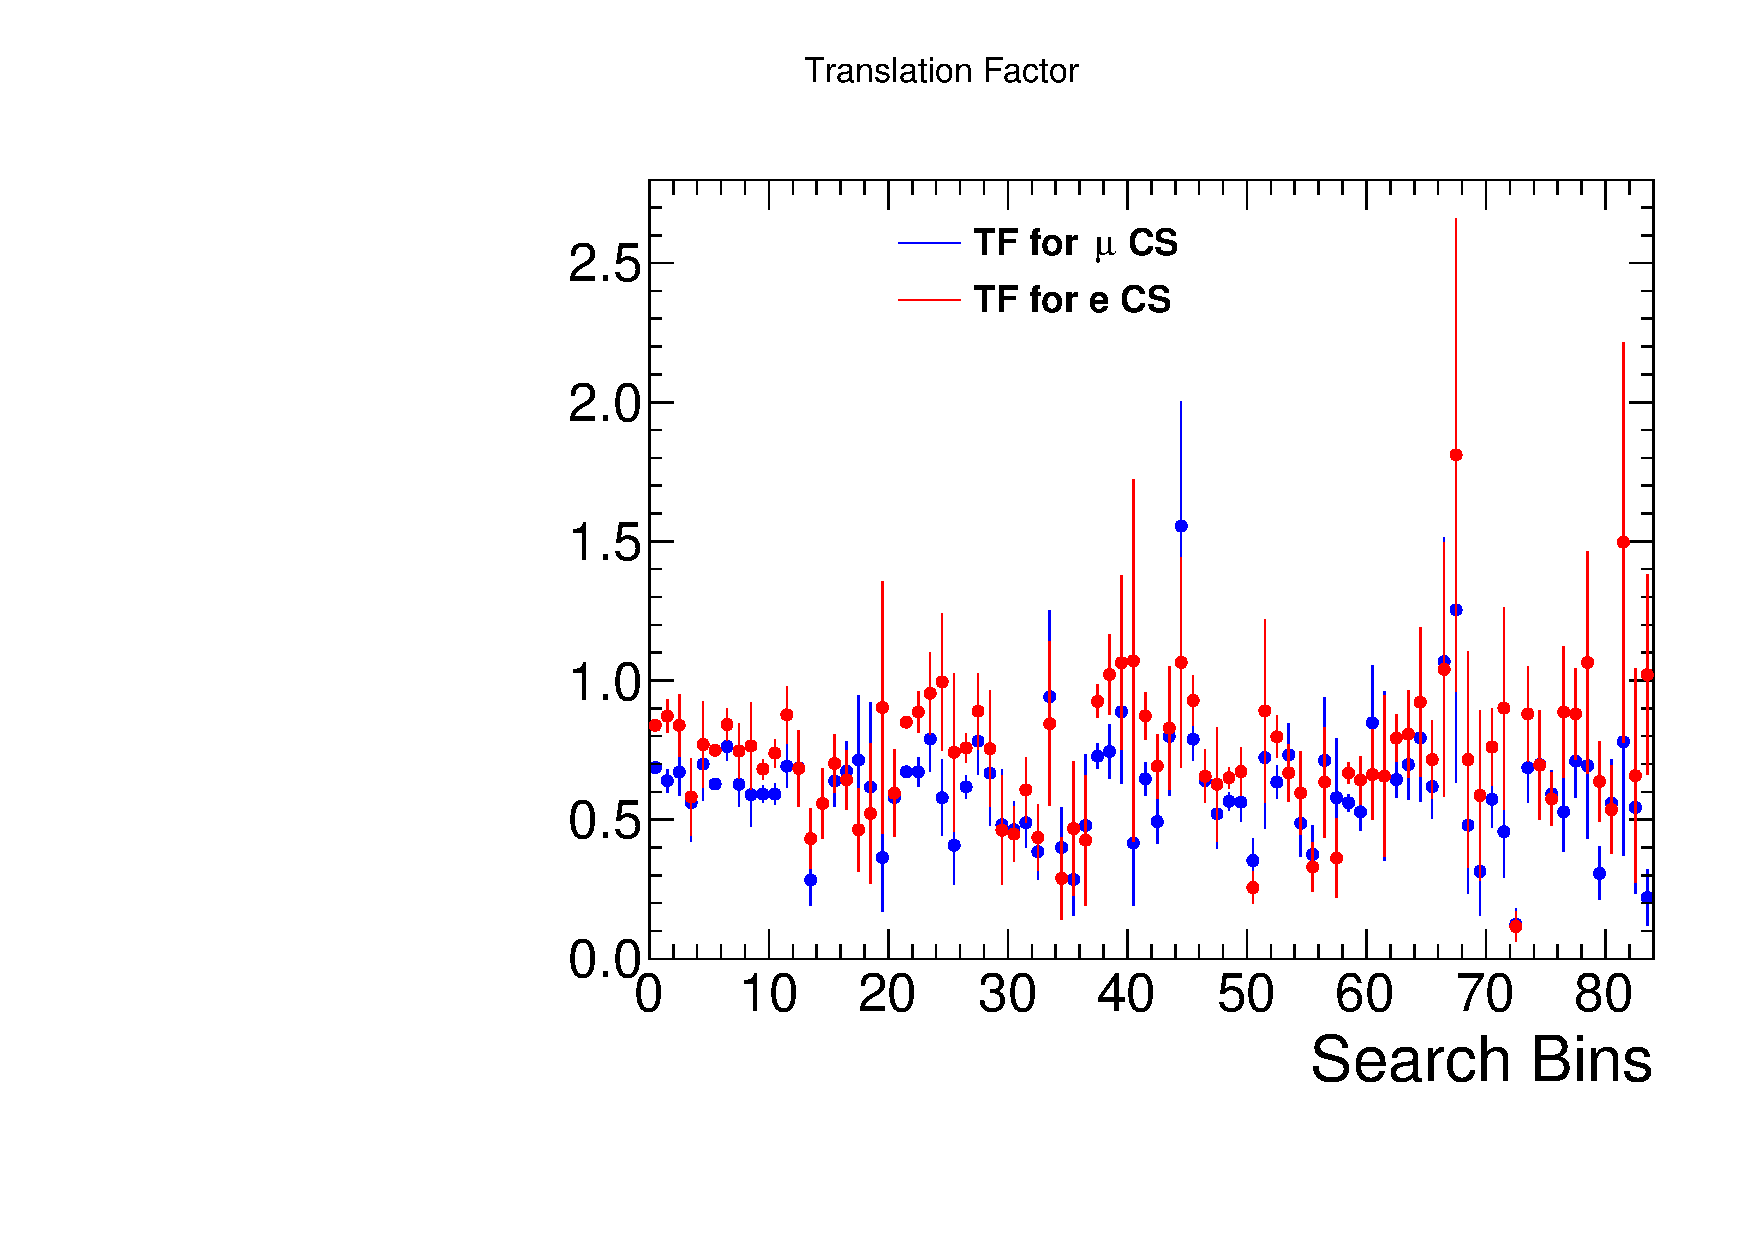
\includegraphics[angle=0,width=0.60\textwidth]{sections/mc4/Backgrounds/TF/figures/comp_TF_hadtau_comb.pdf}
  \end{tabular}
  \caption{Translation factors for the \tauh background prediction with their uncertainties from limited MC statistics for both muon and electron CS.}
    \label{fig:hadtau_TF}
  \end{center}
\end{figure}


\begin{figure}[htbp]
  \begin{center}
  \begin{tabular}{c}
  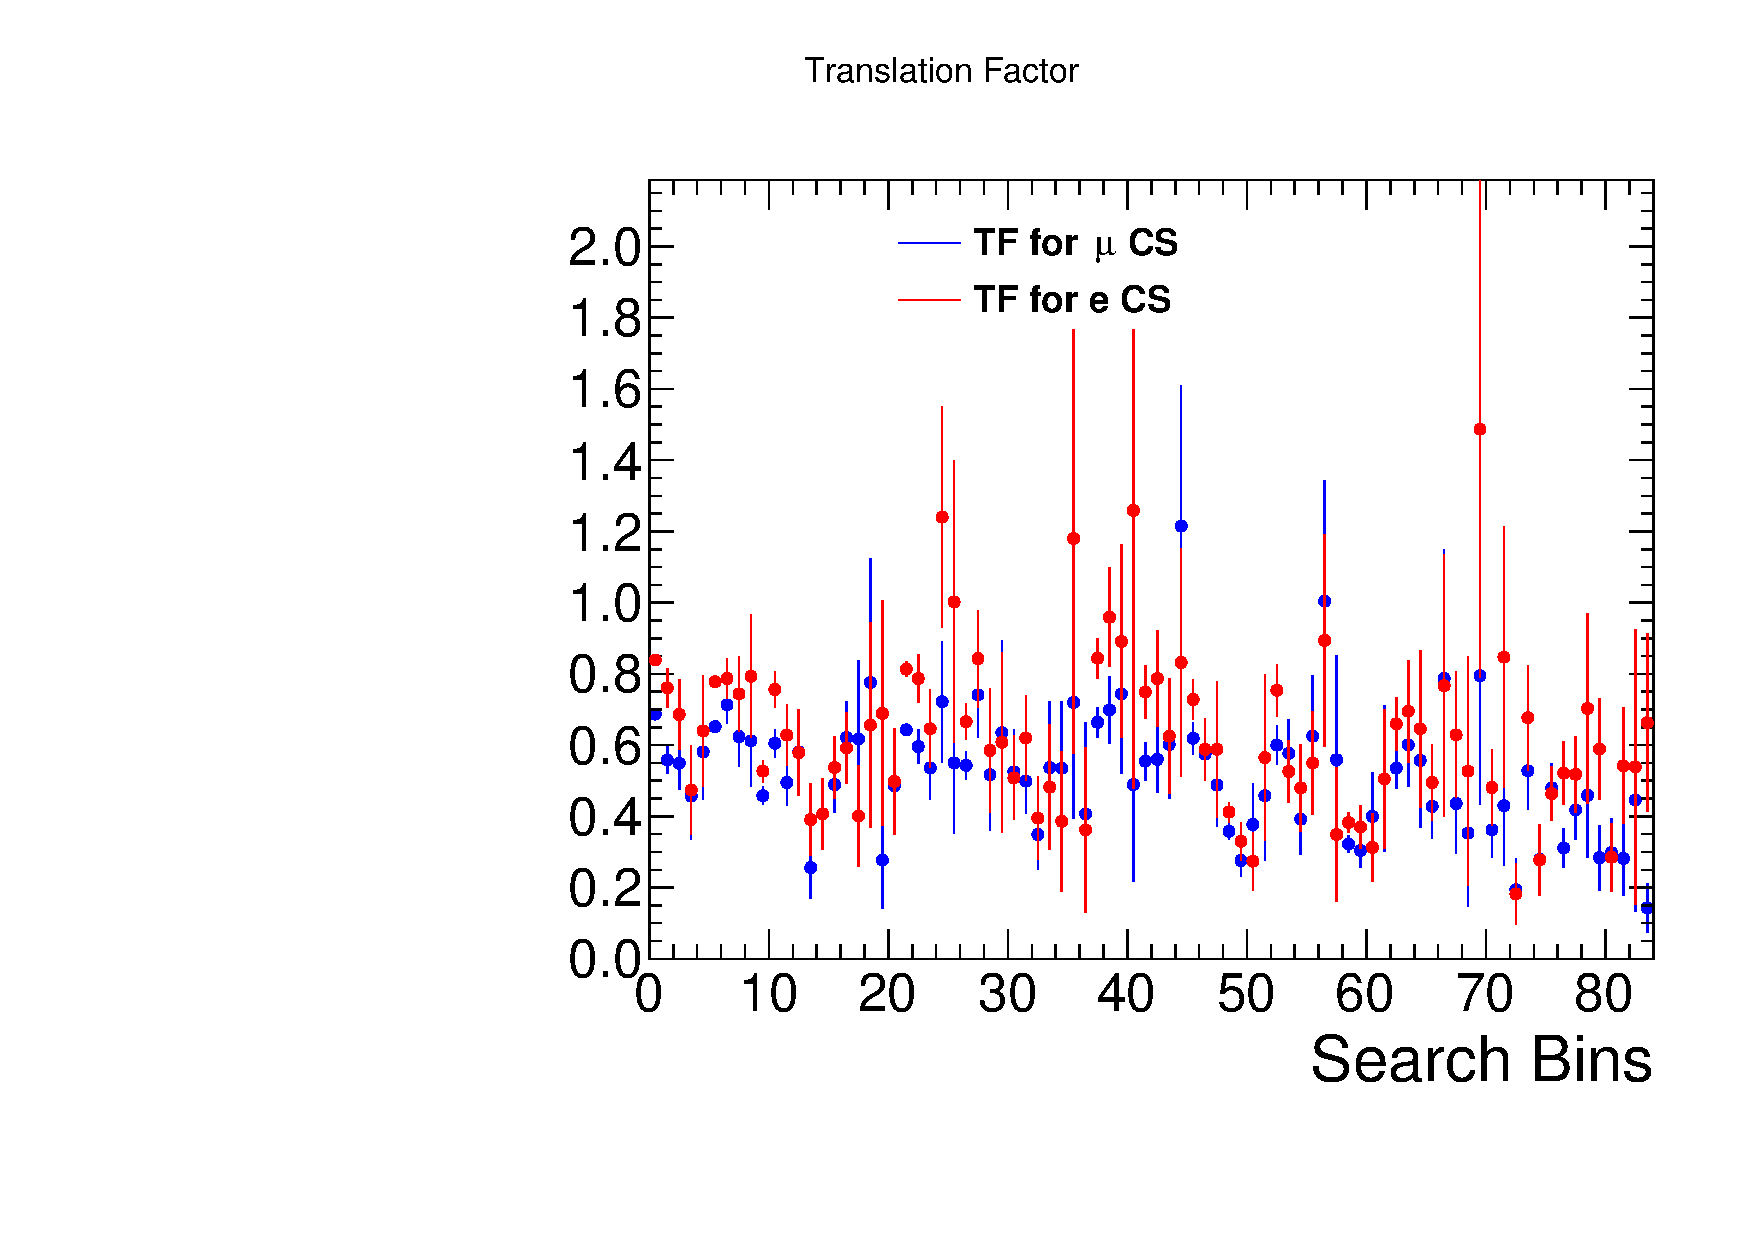
\includegraphics[angle=0,width=0.60\textwidth]{sections/mc4/Backgrounds/TF/figures/comp_TF_lostle_comb.pdf}
  \end{tabular}
  \caption{Translation factors for the lost lepton background prediction with their uncertainties from limited MC statistics for both muon and electron CS.}
    \label{fig:lostle_TF}
  \end{center}
\end{figure}

\begin{figure}[htbp]
  \begin{center}
  \begin{tabular}{cc}
  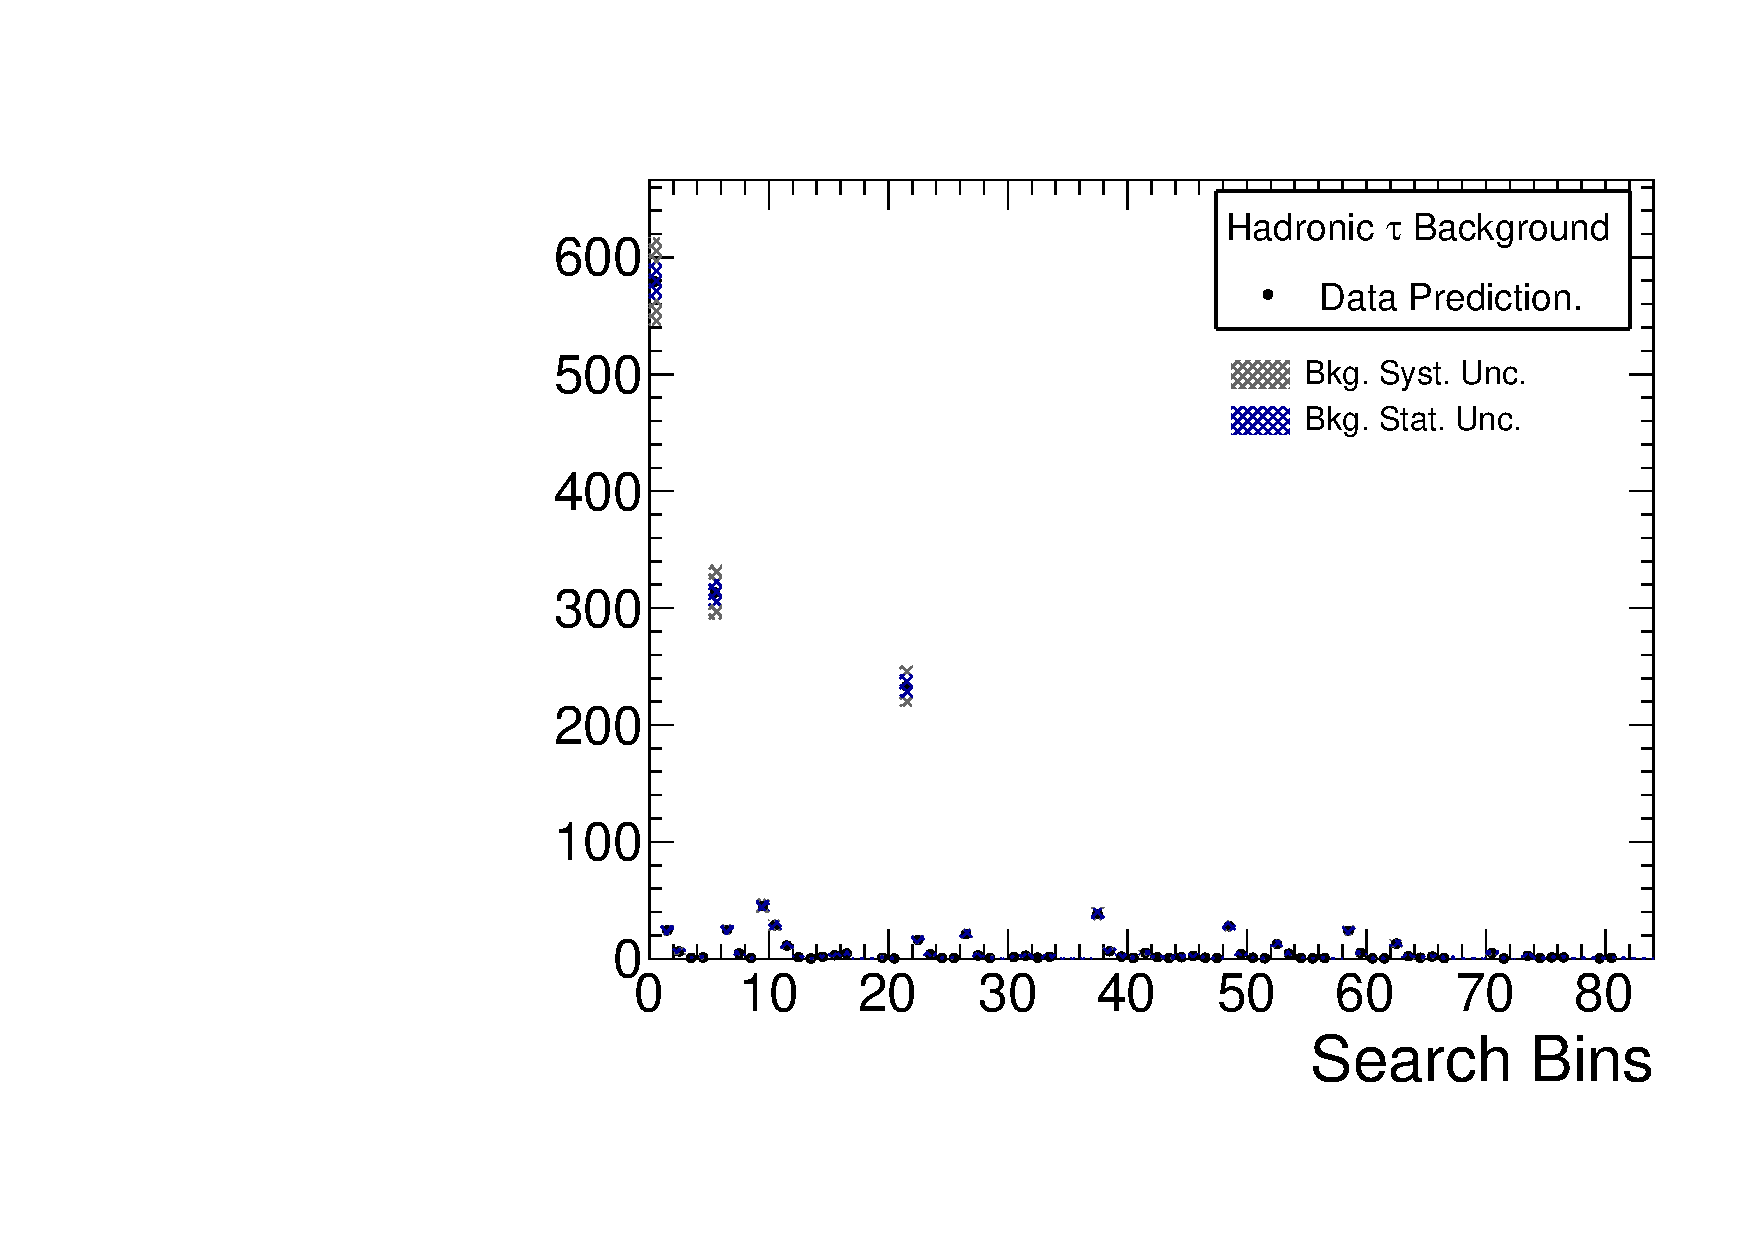
\includegraphics[angle=0,width=0.5\textwidth]{sections/mc4/Backgrounds/TF/figures/pred_full_hadtau_comb.pdf}
  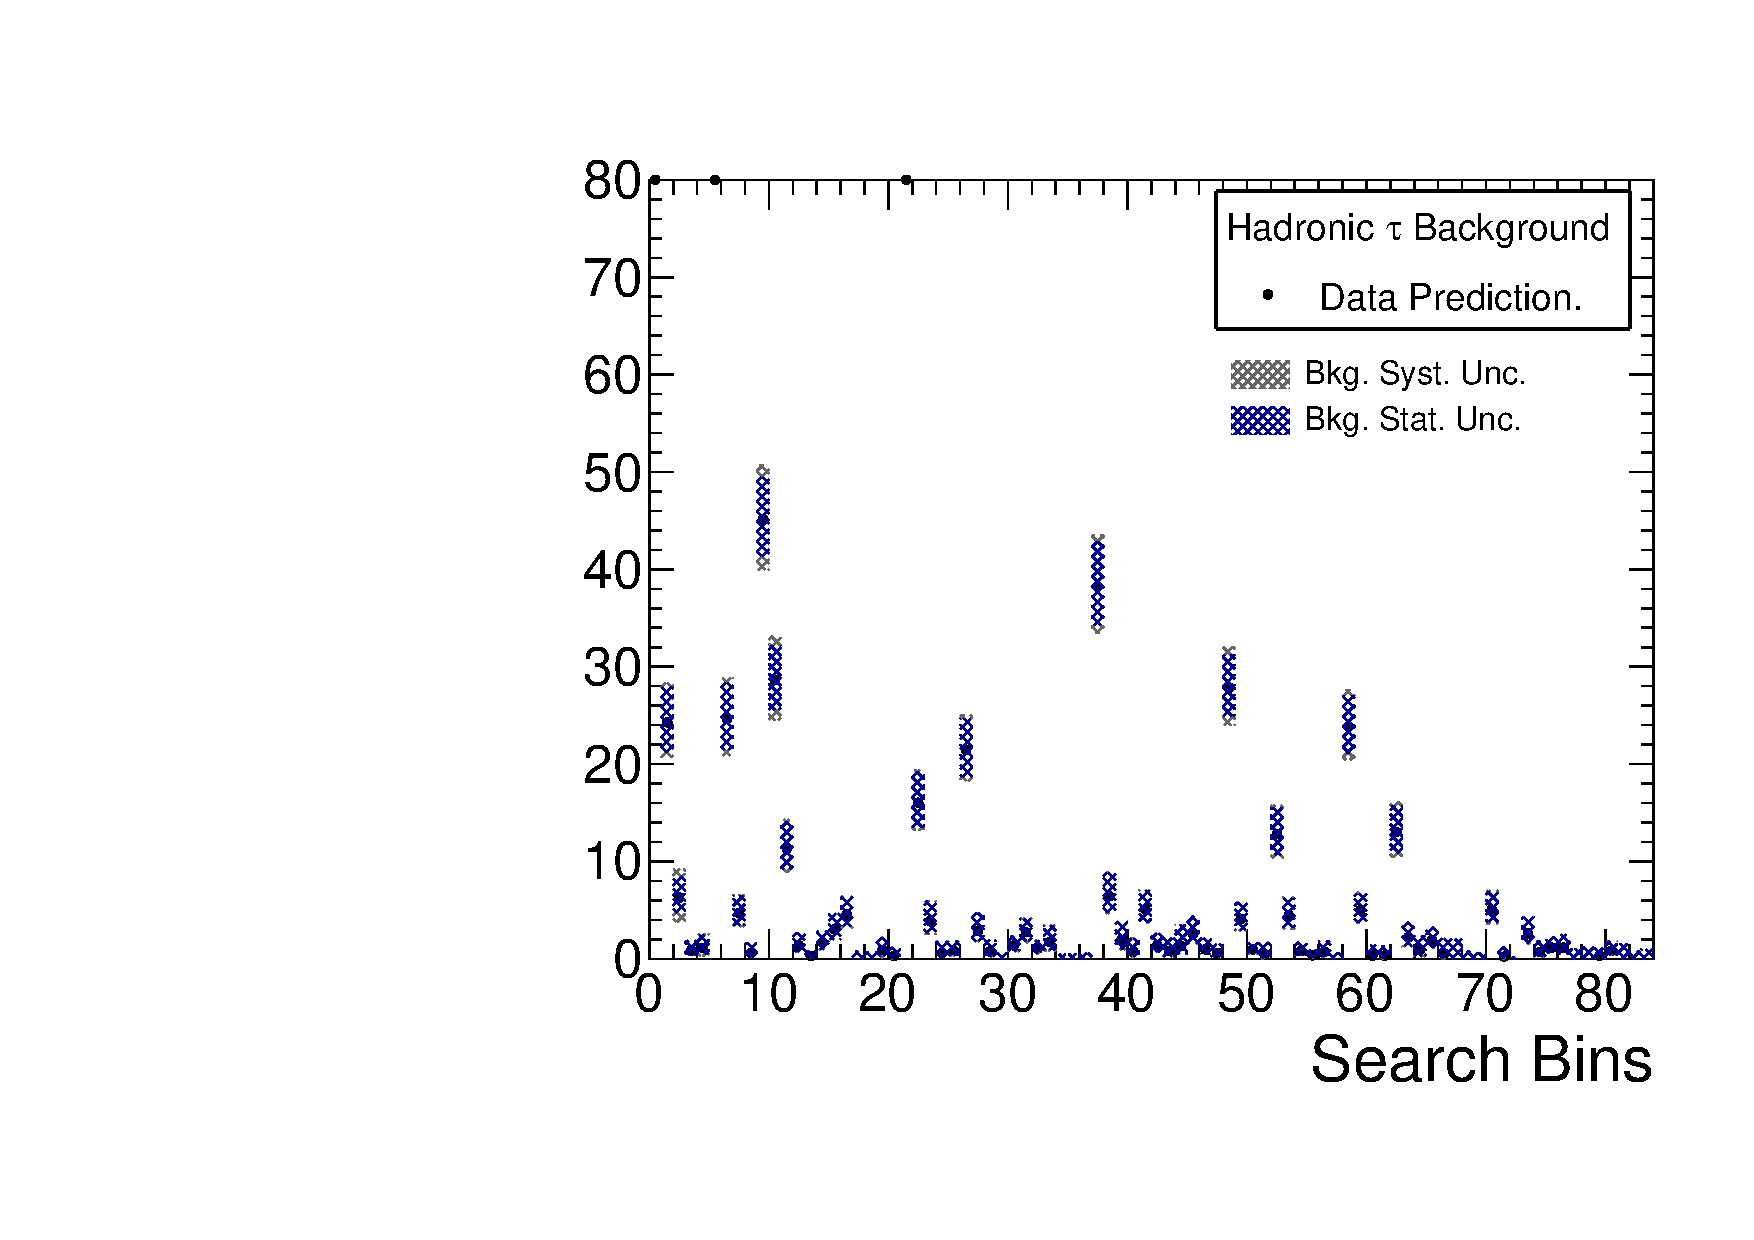
\includegraphics[angle=0,width=0.5\textwidth]{sections/mc4/Backgrounds/TF/figures/pred_zoomin_hadtau_comb.pdf}
  \end{tabular}
  \caption{Predicted hadronic tau background yield for a $35.9$~fb$^{-1}$ data for all the search regions. Right plot is a zoomed version of left plot.
Both statistical and total systematic uncertainties are shown. }
    \label{fig:TAUpredictionSB}
  \end{center}
\end{figure}

\begin{figure}[htbp]
  \begin{center}
  \begin{tabular}{cc}
  \includegraphics[angle=0,width=0.5\textwidth]{sections/mc4/Backgrounds/TF/figures/pred_full_lostle_comb.pdf}
  \includegraphics[angle=0,width=0.5\textwidth]{sections/mc4/Backgrounds/TF/figures/pred_zoomin_lostle_comb.pdf}
  \end{tabular}
  \caption{Predicted lost lepton background yield for a $35.9$~fb$^{-1}$ data for all the search regions. Right plot is a zoomed version of left plot.
Both statistical and total systematic uncertainties are shown. }
    \label{fig:LLpredictionSB}
  \end{center}
\end{figure}


\clearpage
\subsubsection{Classical lost lepton method}
\label{sec:c4bgll}
The classical lost lepton method is a validated method that was used in analysis of the 2015 data\cite{PhysRevD.96.012004}. Although the analysis of the 2016 data uses the simulation based translation factor method for the background estimation for \ttbar, single top and W+jets, the classical method is still an important cross check method. 

The name (lost lepton) of the background is interesting. On one hand, lost lepton indicates leptons that are lost because they are not in the acceptance, not reconstructed or not isolated. On the other hand, a lost lepton is like a lost boy. The boy becomes crazy and finally is misidentified as a jet. The expected numbers of lost lepton events are categorized in Table~\ref{tab:nexpLL}. The numbers of not accepted and not isolated events for muons and electrons are very similar. This is expected because of lepton flavor symmetry among \ttbar decay channels. However, the numbers of not reconstructed muon and electron are very different. The difference comes from the nature of detector: the muons detected by muon system have higher reconstruction efficiencies than electrons in ECAL. 

\begin{table}[htbp]
\fontsize{10 pt}{1.2 em}
\caption{Number of expected lost lepton events (not isolated, not identified/reconstructed and out of the acceptance) in \ttbar, single top and W+jets simulation events, for a luminosity of $35.9$~fb$^{-1}$.} 
\begin{center}
\begin{tabular}{|c|c|c|c|}
\hline
          & iso  & id   & acc \\
\hline
muons     & $139.6\pm16.4$ & $71.3\pm12.5$ & $707.7\pm38.2$ \\
electrons & $148.8\pm17.8$ & $305.2\pm25.3$ & $692.8\pm38.6$ \\
\hline\end{tabular}
\end{center}
\label{tab:nexpLL}
\end{table}

\paragraph{Description of the method}

The lepton identification chain is shown in Fig~\ref{fig:llmethod}. The event will satisfy the lepton veto if the lepton in the event is out of acceptance, not identified, or not isolated. Therefore, we can calculate the acceptance, identification and isolation efficiency in the single lepton control sample in simulation. And then, apply those efficiencies to the single lepton data sample with a model to estimate the lost lepton yield in the search region. 

\begin{figure}[htbp]
\begin{center}
\includegraphics[width=0.55\textwidth]{sections/mc4/Backgrounds/LostLepton/figures/lepton_veto_sketch.png}
\end{center}
\caption{Sketch of the requirements electrons and muons from $W$ decays must meet in order to be rejected by the explicit lepton veto.}
\label{fig:llmethod}
\end{figure}

However, the single lepton control sample can have a large signal contamination for some search bins, i.e., a large contribution of signal events. To reduce the contamination, only events with lepton transverse mass smaller than 100 GeV are considered. The lepton $m_{\rm T}$ is defined in Eq~\ref{eq:MTW}:
\begin{equation}
m_{\rm T} = \sqrt{2 p_{\rm T}(lepton) E^{\rm miss}_{\rm T} (1 - \cos(\Delta \Phi))},
\label{eq:MTW}
\end{equation}
where $\Delta \Phi$ is the distance in $\Phi$ between the muon and the $\MET$. For the electroweak control sample $\MET$ originates from the neutrino, $m_{\rm T}$ represents the transverse $W$-mass ($M_{T}^{W}$), and therefore the distribution falls sharply above $80$~GeV. To compensate for the loss in efficiency due to the $m_{\rm T}$ selection requirement, a correction factor is added in the lost lepton prediction model. 

We also need to consider the events with multiple lost leptons. Here we only estimate a part of the first-order effect: di-muon, di-electron and one electron plut one muon events. Events with a higher number of leptons are not considered. The simplification is reasonable since the correction factor is very close to 1.

As mentioned in the event selection section, an isolated track veto is used to reject 1-prong hadronic tau events. An overall correction factor is applied to account for this selection requirement. 

To summarize, the predicted number of \ttbar, $W$+jets and single top events with lost leptons, $N_{LostLepton}$ contributing to the search sample can be calculated by Eq~\ref{eq:lostleptonequation}:

\begin{equation}
N_{LostLepton}= \sum_{CS} (\sum_{i={e,\mu}}({F_{ISO}}^{i}+{F_{ID}}^{i}+{F_{Acc}}^{i}) \times F_{dilepton}^{i}) \times E_{Mtw} \times \epsilon_{isotrack},
\label{eq:lostleptonequation}
\end{equation}
where $\sum_{CS}$ is the sum over the events in the control sample after the baseline selection, ${F_{ISO}}^{i}$, ${F_{ID}}^{i}$ and ${F_{Acc}}^{i}$ are factors converting the number of events in the control sample to the number of lost lepton events due to respectively isolation, reconstruction or acceptance criteria, $F_{dilepton}^{i}$ is the correction factor for the dilepton contribution, $E_{Mtw}$ is the correction factor for the $M_{T}^{W}$ selection requirement and $\epsilon_{isotrack}$ is the correction factor to compensate for the isolated track veto. The simulation based factors are described in the remainder of this section.

The control sample is normalized to compensate for the reduction of efficiency because of the $M_{T}^{W}<100$~GeV requirement, as illustrated in Table~\ref{tab:mtw}, which shows the $M_{T}^{W}$ correction factors, obtained from simulation, as a function of muon $p_{T}$. 

\begin{table}[htbp]
\fontsize{10 pt}{1.2 em}
\caption{$M_{T}^{W}$ correction factors obtained from \ttbar, single top and W$+$jets simulation, after baseline selection. Only statistical uncertainties are shown.}
\begin{center}
\begin{tabular}{|c|c|c|c|c|c|c|c|}
\hline
\specialcell{Muon \\ $p_T$ [GeV]} & 10-20 & 20-30 & 30-40 & 40-50 & 50-70 & 70-100 & $>100$ \\
\hline
\specialcell{$M_{T}^{W}$ \\ factor} & \specialcell{1.04\\ $\pm$0.01} & \specialcell{1.06\\ $\pm$0.01} & \specialcell{1.07\\ $\pm$0.01} & \specialcell{1.09\\ $\pm$0.01} & \specialcell{1.11\\ $\pm$0.01} & \specialcell{1.19\\ $\pm$0.01} & \specialcell{1.66\\ $\pm$0.02} \\
\hline
\end{tabular}
\end{center}
\label{tab:mtw}
\end{table}

The control sample is weighted according to the lepton isolation efficiency in order to model the non-isolated leptons in the signal region (${F_{ISO}}^{i}$). 
The calculation is for muons and electrons depending on the superscript:
\begin{equation}
{F_{ISO}}^{e/\mu} =  \frac{1-\epsilon_{\rm ISO}^{e/\mu}}{\epsilon_{\rm ISO}^{\mu}} \cdot \frac{\epsilon^{e/\mu}_{\rm ID}}{\epsilon^{\mu}_{\rm ID}} \cdot \frac{\epsilon^{e/\mu}_{\rm Acc}}{\epsilon^{\mu}_{Acc}}.
\label{eq:isolation}
\end{equation}
To model the sample containing no identified electron or muons in the signal region, the control sample is weighted as follows:
\begin{equation}
{F_{ID}}^{e/\mu} = \frac{1}{\epsilon_{\rm ISO}^{\mu}}\cdot \frac{1-\epsilon_{\rm ID}^{e/\mu}}{\epsilon_{\rm ID}^{\mu}}  \cdot \frac{\epsilon^{e/\mu}_{\rm Acc}}{\epsilon^{\mu}_{\rm Acc}}.
\label{eq:id}
\end{equation}

The isolation and reconstruction efficiencies as well as the acceptance are obtained from simulated \ttbar and W$+$jets events. They are measured using reconstructed muons and electrons after the baseline selection and parametrized as a function of the muon $p_T$ and the activity around the lepton, defined as the sum of the $p_{T}$'s of all PF particle candidates in an annulus outside a standard isolation divided by the $p_T$ of the lepton:
\begin{equation}
\textit{$A_{\mu/e}$}=\left(\sum^{R_\texttt{miniIso}<r<0.4}_\texttt{PFcands} p_\text{T}\right) / p_\text{T}(lep) \; .
\label{eq:activity}
\end{equation}

The lepton isolation and reconstruction efficiencies are analysis independent. Therefore, they are calculated without the baseline selection. They are shown in Figs~\ref{fig:muoneffiso},~\ref{fig:eleeffiso},~\ref{fig:muoneffreco} and~\ref{fig:eleeffreco}.

\begin{figure}[hptb]
\begin{center}
\begin{tabular}{c}
\includegraphics[width=1.0\textwidth]{sections/mc4/Backgrounds/LostLepton/figures/v3_2d_effs_mus_iso_no_baseline.pdf}
\end{tabular}
\end{center}
\caption{Muon isolation efficiencies as a function of the muon $p_T$ and the activity around the muon. Only statistical uncertainties are shown.}
\label{fig:muoneffiso}
\end{figure}

\begin{figure}[hptb]
\begin{center}
\begin{tabular}{c}
\includegraphics[width=1.0\textwidth]{sections/mc4/Backgrounds/LostLepton/figures/v3_2d_effs_els_iso_no_baseline.pdf}
\end{tabular}
\end{center}
\caption{Electron isolation efficiencies as a function of the electron $p_T$ and the activity around the electron. Only statistical uncertainties are shown.}
\label{fig:eleeffiso}
\end{figure}

\begin{figure}[hptb]
\begin{center}
\begin{tabular}{c}
\includegraphics[width=1.0\textwidth]{sections/mc4/Backgrounds/LostLepton/figures/v3_2d_effs_mus_reco_no_baseline.pdf}
\end{tabular}
\end{center}
\caption{Muon reconstruction efficiencies as a function of the muon $p_T$ and Eta. Only statistical uncertainties are shown.}
\label{fig:muoneffreco}
\end{figure}

\begin{figure}[hptb]
\begin{center}
\begin{tabular}{c}
\includegraphics[width=1.0\textwidth]{sections/mc4/Backgrounds/LostLepton/figures/v3_2d_effs_els_reco_no_baseline.pdf}
\end{tabular}
\end{center}
\caption{Electron reconstruction efficiencies as a function of the electron $p_T$ and Eta. Only statistical uncertainties
are shown.}
\label{fig:eleeffreco}
\end{figure}

Another multiplicative factor to the number of control region events originates from leptons that 
are out of acceptance. Such events occur when leptons have a transverse 
momentum below the lepton veto $p_{T}$ threshold or when leptons are emitted in 
the forward region outside the $\eta$ acceptance. %, or when electrons are emitted in the transition reigion.
For example, leptons from leptonic-tau decays tend to have low 
momentum as well as neutrinos that contribute to the event \MET. 
This ${F_{Acc}}^{e/\mu}$ factor is modeled according to the following equation:
\begin{equation}
{F_{Acc}}^{e/\mu} = \frac{1}{\epsilon_{\rm ISO}^{\mu}}\cdot \frac{1}{\epsilon_{\rm ID}^{\mu}}  \cdot \frac{1 - \epsilon^{e/\mu}_{\rm Acc}}{\epsilon^{\mu}_{\rm Acc}}
\label{eq:accept}
\end{equation}
The acceptance efficiencies are derived for each search bin 
from \ttbar and W$+$jets simulated events,
selected using the baseline criteria. 
They are shown in Fig~\ref{fig:acceptance}.

\begin{figure}[hptb]
\begin{center}
\includegraphics[width=0.9\textwidth]{sections/mc4/Backgrounds/LostLepton/figures/v2_acc_eff_84bins.pdf}%\\
\end{center}
\caption{Acceptance efficiencies for muons and electrons in each of the
search bins. Only the statistical uncertainties are shown.}
\label{fig:acceptance}
\end{figure}

The \ttbar samples include both semileptonic/dileptonic "inclusive" samples and HT-binned samples.
The \ttbar inclusive samples have the largest weight when the samples are combined.
However, the \ttbar inclusive samples have very few events in some bins, which dramatically influences the efficiences.
We therefore set a criterion in the acceptance and isolated track efficiency calculations that if there are less than five events in a search bin, the acceptance and isolated track efficiencies are calculated for that bin using only the HT-binned samples.

Dilepton events may also contribute to the background if both leptons are lost.
In the muon control sample, there are dilepton events that contribute 
when one lepton is lost while the other one is reconstructed and
identified as a muon.

If $\epsilon_{\mu}$ is the total muon efficiency 
(reco/identification times acceptance), then the 1-muon control sample contains:
\begin{itemize}
\item $\epsilon_{\mu}$ events with exactly one identified/isolated muon and 
no other lost lepton.
\item $2\epsilon_{\mu}(1-\epsilon_{\mu})$ events with one identified/isolated 
muon and one lost muon.
\item $2\epsilon_{\mu}(1-\epsilon_{e})$ events with one muon and one 
lost electron.
\end{itemize}
For these events we apply a $(1-\epsilon_{\mu})/\epsilon_{\mu}$ factor to
predict the number of events with  
lost muons and  $(1-\epsilon_{e})/\epsilon_{\mu}$ to predict the
number of lost electrons.
This leads to an overestimate in the number of lost dileptonic events in the 
prediction by a factor of two:
\begin{itemize}
\item Two lost muons case: prediction is 
$2(1-\epsilon_{\mu})(1-\epsilon_{\mu})$, expectation 
is $(1-\epsilon_{\mu})(1-\epsilon_{\mu})$.
\item Two lost electrons case: prediction is 
$2(1-\epsilon_{e})(1-\epsilon_{e})$, 
expectation is $(1-\epsilon_{e})(1-\epsilon_{e})$.
\item One lost muon and one lost electron case: prediction is
$4(1-\epsilon_{\mu})(1-\epsilon_{e})$, 
expectation is $2(1-\epsilon_{\mu})(1-\epsilon_{e})$.
\end{itemize}
This effect is evaluated in  
simulated \ttbar, single top and W$+$jets events as the ratio between the number of events 
with one or two lost leptons over the number of events with one lost 
lepton plus twice the number of events with two lost lepton. 
Separate correction factors are applied,  
$F_{dilepton}^{\mu}$=$ (99.4\pm0.7)\% $ for muons and 
$F_{dilepton}^{e}$=$ (97.1\pm0.9)\% $ for electrons.

The purity of the electron control sample is measured in simulation and found to be $0.96\pm0.01$. The purity of the muon control sample is assumed to be 1.

Finally, the isolated track veto efficiency factor is applied in 
Eq~\ref{eq:lostleptonequation}
to get the final number of predicted lost lepton background events.
The isolated track veto efficiency is computed from simulated events 
for each search bin and shown in Fig~\ref{fig:isotrackeff}.

\begin{figure}[htbp]
\begin{center}
\includegraphics[width=0.9\textwidth]{sections/mc4/Backgrounds/LostLepton/figures/v2_isotrackvetoEff.pdf}%\\
\end{center}
\caption{Isolated track veto efficiencies for each search bin.}
\label{fig:isotrackeff}
\end{figure}

\paragraph{Closure Test}
Closure tests have been performed using \ttbar, single top and W$+$jets Monte Carlo samples. The prediction, i.e. the number of events obtained using the lost lepton 
method explained in the previous section is compared with the expectation, i.e. the true number of Monte Carlo simulated events with one or two lost leptons (coming from the $W$ boson produced in top quark decays). 

The results of the closure test are shown in Fig~\ref{fig:closureSBisotrk}. The expectation/prediction disagreements are propagated into the systematic uncertainty, and is the major uncertainty in the lost lepton background estimation.

\begin{figure}[htbp]
\begin{center}
\begin{tabular}{c}
\includegraphics[width=0.85\textwidth, height=0.35\textheight]{sections/mc4/Backgrounds/LostLepton/figures/v3_closure_mu_cs.pdf}\\
\includegraphics[width=0.85\textwidth, height=0.35\textheight]{sections/mc4/Backgrounds/LostLepton/figures/v3_closure_el_cs.pdf}
\end{tabular}
\end{center}
\caption{The lost lepton background in all the search regions of the analysis as predicted directly from \ttbar, single top and W$+$jets simulation (in red) and as predicted by applying the lost lepton background-determination procedure to simulated muon control sample (in black). The lower panel shows the ratio between the true and predicted yields. The top plot shows the prediction computed from the muon control sample. The bottom plot shows the prediction from the electron control sample.}
\label{fig:closureSBisotrk}
\end{figure}

\paragraph{Systematic uncertainties}

The following systematic uncertainties are included for the lost lepton background prediction:

\begin{itemize}
\item Lepton isolation efficiency:\\
  The muon and electron isolation efficiencies are obtained from simulated events. In order to estimate how well data and simulation agree, Tag-and-Probe efficiencies on the Z resonance from data and simulation are used, which are provided by the SUSY lepton scale-factor group. The maximum between the uncertainty obtained with the Tag-and-Probe comparing Data and simulation and the uncertainty on this value is used.
  Since no systematic bias is visible,
  no correction based on data/simulation scaling factors is introduced, and we merely take into account the systematic uncertainty obtained by propagating the SUSY lepton scale-factor group numbers.
  In addition the statistical uncertainty in the simulation efficiencies are
  propagated the same way as the Tag-and-Probe uncertainty.
  \item Lepton reconstruction/ID efficiency:\\
  The muon and electron reconstruction and ID efficiencies are obtained from simulated events. The main uncertainty here arises
  from possible differences between efficiencies obtained from data and simulation. By examining the reconstruction efficiencies as a function of the search variables it seems to be reasonable that using some inclusive efficiencies also provided by the SUSY lepton scale-factor groups are sufficient for deriving data/simulation uncertainties (same procedure as above). Furthermore, the statistical uncertainties from simulation are propagated.
\item Lepton acceptance:\\
  The uncertainty in the acceptance efficiency consists of the uncertainty
  in the parton distribution functions (PDF), the simulation renormalization/factorization scale
  and the uncertainty arising from the statistical precision of the efficiency maps.
  The PDF uncertainties are studied by varying the PDF sets used to produce the
  simulation samples, according to their uncertainties in the baseline selection.
\item Control sample purity:\\
The purity is expected to be very high ($>99\%$) so this only leads to a minor systematic uncertainty and a conservative uncertainty of 20\% on the impurity is assigned. Furthermore, the statistical uncertainties from simulation are propagated.
\item Dilepton correction:\\
Both dileptonic corrections are only minor compared to the remaining ones so a conservative systematic uncertainty is assigned here.
An uncertainty of 50\% is assigned on the number of di-leptonic events. Furthermore, the statistical uncertainties from simulation are propagated.
\item $M_T$ cut efficiency:\\
  The uncertainty associated with the \MT cut consists of two parts: the statistical uncertainty in the efficiency map from simulation and a systematic uncertainty. For the latter, the uncertainty in the jet energy corrections (JEC) is propagated to \MET (following the latest recommendations of the MET group) and the efficiency of the $M_T$ cut is recalculated. Following this procedure, a conservative uncertainty of 1\% is assigned as a systematic uncertainty. 
\item Isolated-track vetoes:\\
  The isolated-track vetoes lead to a reduction of about 40\%
  of the lost lepton background. Due to the size of this reduction,
  it is important to study the validity of the efficiency maps. A detailed study has been performed in the context of the RA2/b analysis~\cite{Sirunyan:2017cwe} comparing Tag-and-Probe efficiencies on the Z resonance from data and simulation. This study has shown that a systematic uncertainty of 10\% is a conservative estimate for the systematic uncertainty on the number of events removed by the isolated track veto.
\item simulation closure:\\
Furthermore, an uncertainty in the precision of the simulation closure test is assigned. Since no true non-closure is observed (see Fig~\ref{fig:closureSBisotrk}) the larger value of the non-closure or the statistical uncertainty in the non-closure is assigned for each bin. 
\end{itemize}

The source and contribution of the different components of the lost lepton method systematic uncertainties are shown in Table~\ref{tab:systematics}.

\begin{table}[htbp]
\fontsize{10 pt}{1.2 em}
\caption{Source and contribution of the different components of the lost lepton method systematic uncertainties.} 
\begin{center}
\begin{tabular}{|c|c|c|c|}
\hline
Source & Note & \specialcell{Electron \\ control sample} & \specialcell{Muon \\ control sample} \\
\hline
Muon Iso 			& \specialcell{Data-MC correction \\ from tag and probe} & 1\% to 3\% & 1\% to 4\% \\
\hline
Elec Iso 			& \specialcell{Data-MC correction \\ from tag and probe} & 4\% to 8\% & 2\% to 5\% \\
\hline
Muon ID 			& \specialcell{Data-MC correction \\ from tag and probe} & 2\% to 7\% & 4\% to 11\% \\
\hline
Elec ID 			& \specialcell{Data-MC correction \\ from tag and probe} & 6\% to 11\% & 2\% to 8\% \\
\hline
Acceptance    & \specialcell{PDF and MC \\ scale variation} & 4\% to 97\% & 4\% to 97\% \\ 
\hline
\specialcell{Other SM \\ contribution}  & \specialcell{20\% uncertainty on the purity} & 0\% & 0\% \\
\hline
\specialcell{Di-Muon \\ Correction}     & \specialcell{Statistical uncertainty + 50\%} & 0\% & 0\% \\
\hline
\specialcell{Di-Electron \\ Correction} & \specialcell{Statistical uncertainty + 50\%} & 1\% & 1\% \\
\hline
\specialcell{Transverse \\ Mass Cut}    & \specialcell{Variation of \MET energy scale} & 0\% & 0\% \\
\hline
\specialcell{Isolated \\ track veto}    & \specialcell{Data-MC correction \\ on isolated track \\ veto efficiencies} & 10\% & 10\% \\
\hline
Closure & \specialcell{Non-closure and \\ statistical precision \\ of the closure} & 2\% to 104\% & 2\% to 86\% \\
\hline
Total	& & 13\% to 143\% & 12\% to 131\% \\
\hline
\end{tabular}
\end{center}
\label{tab:systematics}
\end{table}

\paragraph{Lost Lepton background prediction}

The lost lepton method is applied to data event samples (collected with the search triggers) corresponding to an integrated luminosity of $35.9$~fb$^{-1}$. The final predictions for all search bins are shown in Figs~\ref{fig:LostLeptonResult_mu} and \ref{fig:LostLeptonResult_el} (red points) and listed in Tables~\ref{tab:LLpredmu1}-\ref{tab:LLpredel3} for both the muon and electron channels.

Applying the procedure indicated by Eq.~\ref{eq:lostleptonequation}, each event in the control sample is weighted by the various efficiencies. 
A few bins have zero predicted events. In that case the statistical uncertainty is computed as the upper bound of the statistical uncertainty on 0 given by the Garwood interval (1.8) multiplied by the average translation factor to go from a raw number of events to the prediction. This Poisson uncertainty is treated in the Higgs combination tool using a gamma function~\cite{HiggsCombine,cms-note-2011-005}.

\begin{figure}[hptb]
\begin{center}
\begin{tabular}{c}
\includegraphics[width=0.50\textwidth]{sections/mc4/Backgrounds/LostLepton/figures/v4_DataCardCampare_0_700_mu_cs.pdf}\\
\includegraphics[width=0.40\textwidth]{sections/mc4/Backgrounds/LostLepton/figures/v4_DataCardCampare_0_50_mu_cs.pdf}
\includegraphics[width=0.40\textwidth]{sections/mc4/Backgrounds/LostLepton/figures/v4_DataCardCampare_0_700_mu_cs_log.pdf}
\end{tabular}
\end{center}
\caption{Lost lepton background predictions on muon control sample, in red. The blue points are the results obtained with the average TF method. The uncertainties include both the statistical and systematic uncertainties. Bottom left plot is a zoom of the top plot and the bottom right plot is log sacle.}
\label{fig:LostLeptonResult_mu}
\end{figure}

\begin{figure}[hptb]
\begin{center}
\begin{tabular}{c}
\includegraphics[width=0.50\textwidth]{sections/mc4/Backgrounds/LostLepton/figures/v4_DataCardCampare_0_700_el_cs.pdf}\\
\includegraphics[width=0.40\textwidth]{sections/mc4/Backgrounds/LostLepton/figures/v4_DataCardCampare_0_50_el_cs.pdf}
\includegraphics[width=0.40\textwidth]{sections/mc4/Backgrounds/LostLepton/figures/v4_DataCardCampare_0_700_el_cs_log.pdf}
\end{tabular}
\end{center}
\caption{Lost lepton background predictions on electron control sample, in red. The blue points are the results obtained with the average TF method. The uncertainties include both the statistical and systematic uncertainties. Bottom left plot is a zoom of the top plot and the bottom right plot is log sacle.}
\label{fig:LostLeptonResult_el}
\end{figure}

\begin{table}[htbp]
\fontsize{10 pt}{1.2 em}
\selectfont
\begin{centering}
\caption{\label{tab:LLpredmu1} Predicted lost lepton background yield from the muon control sample with statistical and systematic uncertainties for a $35.9$~fb$^{-1}$ sample.}
\hspace*{-4ex}
\begin{tabular}{|c|c|c|c|c||c|}
\hline
Search Bin & \ntops & \nbjets & \MTTwo [GeV] & \MET [GeV] & Lost Lepton Prediction\\
\hline
0 &               1 &               1 &         200-300 &         250-400 & 571.615 $^{+21.270}_{-21.237}$ $^{+80.824}_{-85.452}$ \\ 
\hline
1 &               1 &               1 &         200-300 &         400-500 & 24.355 $^{+4.936}_{-4.837}$ $^{+4.015}_{-4.201}$ \\ 
\hline
2 &               1 &               1 &         200-300 &         500-600 & 2.376 $^{+1.520}_{-1.070}$ $^{+0.669}_{-0.682}$ \\ 
\hline
3 &               1 &               1 &         200-300 &         600-750 & 0.331 $^{+0.824}_{-0.331}$ $^{+0.182}_{-0.183}$ \\ 
\hline
4 &               1 &               1 &         200-550 &            750+ & 0.231 $^{+0.607}_{-0.231}$ $^{+0.150}_{-0.150}$ \\ 
\hline
5 &               1 &               1 &         300-400 &         250-400 & 332.123 $^{+16.111}_{-16.070}$ $^{+47.094}_{-49.965}$ \\ 
\hline
6 &               1 &               1 &         300-400 &         400-500 & 25.202 $^{+4.961}_{-4.816}$ $^{+4.242}_{-4.427}$ \\ 
\hline
7 &               1 &               1 &         300-400 &         500-600 & 5.341 $^{+2.178}_{-1.815}$ $^{+1.749}_{-1.773}$ \\ 
\hline
8 &               1 &               1 &         300-400 &         600-750 & 0.894 $^{+1.127}_{-0.645}$ $^{+0.369}_{-0.372}$ \\ 
\hline
9 &               1 &               1 &         400-550 &         250-400 & 36.205 $^{+5.030}_{-4.960}$ $^{+8.485}_{-8.724}$ \\ 
\hline
10 &               1 &               1 &         400-550 &         400-500 & 36.177 $^{+5.448}_{-5.329}$ $^{+7.466}_{-7.691}$ \\ 
\hline
11 &               1 &               1 &         400-550 &         500-600 & 7.748 $^{+2.303}_{-2.102}$ $^{+1.895}_{-1.937}$ \\ 
\hline
12 &               1 &               1 &         400-550 &         600-750 & 1.306 $^{+1.277}_{-0.924}$ $^{+0.449}_{-0.453}$ \\ 
\hline
13 &               1 &               1 &         550-750 &         250-400 & 0.609 $^{+0.681}_{-0.445}$ $^{+0.632}_{-0.633}$ \\ 
\hline
14 &               1 &               1 &         550-750 &         400-500 & 0.432 $^{+0.756}_{-0.432}$ $^{+0.185}_{-0.187}$ \\ 
\hline
15 &               1 &               1 &         550-750 &         500-600 & 2.232 $^{+1.523}_{-1.234}$ $^{+0.705}_{-0.719}$ \\ 
\hline
16 &               1 &               1 &         550-750 &         600-750 & 2.293 $^{+1.551}_{-1.177}$ $^{+0.674}_{-0.688}$ \\ 
\hline
17 &               1 &               1 &         550-750 &            750+ & 0.000 $^{+0.990}_{-0.000}$ $^{+0.000}_{-0.000}$ \\ 
\hline
18 &               1 &               1 &            750+ &         250-600 & 0.000 $^{+1.661}_{-0.000}$ $^{+0.000}_{-0.000}$ \\ 
\hline
19 &               1 &               1 &            750+ &         600-750 & 0.000 $^{+0.992}_{-0.000}$ $^{+0.000}_{-0.000}$ \\ 
\hline
20 &               1 &               1 &            750+ &            750+ & 0.446 $^{+1.055}_{-0.446}$ $^{+0.243}_{-0.244}$ \\ 
\hline
21 &               1 &               2 &         200-350 &         250-400 & 207.008 $^{+12.950}_{-12.904}$ $^{+28.139}_{-29.923}$ \\ 
\hline
22 &               1 &               2 &         200-350 &         400-500 & 10.922 $^{+2.757}_{-2.558}$ $^{+2.101}_{-2.173}$ \\ 
\hline
23 &               1 &               2 &         200-350 &         500-600 & 3.971 $^{+2.797}_{-2.627}$ $^{+1.238}_{-1.259}$ \\ 
\hline
24 &               1 &               2 &         200-350 &         600-750 & 1.471 $^{+1.617}_{-1.043}$ $^{+0.595}_{-0.598}$ \\ 
\hline
25 &               1 &               2 &         200-650 &            750+ & 0.796 $^{+1.127}_{-0.563}$ $^{+0.694}_{-0.700}$ \\ 
\hline
26 &               1 &               2 &         350-450 &         250-400 & 18.915 $^{+3.488}_{-3.308}$ $^{+5.244}_{-5.348}$ \\ 
\hline
27 &               1 &               2 &         350-450 &         400-500 & 4.115 $^{+2.637}_{-2.118}$ $^{+1.215}_{-1.231}$ \\ 
\hline
28 &               1 &               2 &         350-450 &         500-600 & 0.000 $^{+1.057}_{-0.000}$ $^{+0.000}_{-0.000}$ \\ 
\hline
29 &               1 &               2 &         350-450 &         600-750 & 0.000 $^{+1.090}_{-0.000}$ $^{+0.000}_{-0.000}$ \\ 
\hline
30 &               1 &               2 &         450-650 &         250-400 & 1.269 $^{+1.452}_{-0.926}$ $^{+0.692}_{-0.695}$ \\ 
\hline
31 &               1 &               2 &         450-650 &         400-500 & 0.000 $^{+0.884}_{-0.000}$ $^{+0.000}_{-0.000}$ \\ 
\hline
32 &               1 &               2 &         450-650 &         500-600 & 0.519 $^{+0.701}_{-0.370}$ $^{+0.184}_{-0.185}$ \\ 
\hline
33 &               1 &               2 &         450-650 &         600-750 & 0.482 $^{+1.016}_{-0.482}$ $^{+0.352}_{-0.353}$ \\ 
\hline
34 &               1 &               2 &            650+ &         250-600 & 0.000 $^{+1.282}_{-0.000}$ $^{+0.000}_{-0.000}$ \\ 
\hline
35 &               1 &               2 &            650+ &         600-750 & 0.000 $^{+1.123}_{-0.000}$ $^{+0.000}_{-0.000}$ \\ 
\hline
36 &               1 &               2 &            650+ &            750+ & 0.000 $^{+0.953}_{-0.000}$ $^{+0.000}_{-0.000}$ \\ 
\hline
\end{tabular}
\par\end{centering}
\end{table}

\begin{table}[htbp]
\fontsize{10 pt}{1.2 em}
\selectfont
\begin{centering}
\caption{\label{tab:LLpredmu2} Predicted lost lepton background yield from the muon control sample with statistical and systematic uncertainties for a $35.9$~fb$^{-1}$ sample.}
\hspace*{-4ex}
\begin{tabular}{|c|c|c|c|c||c|}
\hline
37 &               1 &              3+ &        300-1000 &         250-350 & 35.608 $^{+5.692}_{-5.569}$ $^{+6.655}_{-6.875}$ \\ 
\hline
38 &               1 &              3+ &        300-1000 &         350-450 & 8.699 $^{+3.703}_{-3.514}$ $^{+1.994}_{-2.035}$ \\ 
\hline
39 &               1 &              3+ &        300-1000 &         450-550 & 1.120 $^{+1.490}_{-0.792}$ $^{+0.472}_{-0.476}$ \\ 
\hline
40 &               1 &              3+ &        300-1000 &            550+ & 0.440 $^{+0.908}_{-0.440}$ $^{+0.330}_{-0.331}$ \\ 
\hline
41 &               1 &              3+ &       1000-1500 &         250-350 & 7.396 $^{+2.601}_{-2.400}$ $^{+1.654}_{-1.697}$ \\ 
\hline
42 &               1 &              3+ &       1000-1500 &         350-450 & 0.000 $^{+0.992}_{-0.000}$ $^{+0.000}_{-0.000}$ \\ 
\hline
43 &               1 &              3+ &       1000-1500 &         450-550 & 1.118 $^{+1.319}_{-0.827}$ $^{+0.589}_{-0.592}$ \\ 
\hline
44 &               1 &              3+ &       1000-1500 &            550+ & 0.520 $^{+1.291}_{-0.520}$ $^{+0.674}_{-0.674}$ \\ 
\hline
45 &               1 &              3+ &           1500+ &         250-350 & 1.366 $^{+1.192}_{-0.818}$ $^{+0.459}_{-0.467}$ \\ 
\hline
46 &               1 &              3+ &           1500+ &         350-550 & 0.777 $^{+1.127}_{-0.553}$ $^{+0.449}_{-0.451}$ \\ 
\hline
47 &               1 &              3+ &           1500+ &            550+ & 0.626 $^{+1.199}_{-0.626}$ $^{+0.321}_{-0.325}$ \\ 
\hline
\end{tabular}
\par\end{centering}
\end{table}

\begin{table}[htbp]
\fontsize{10 pt}{1.2 em}
\selectfont
\begin{centering}
\caption{\label{tab:LLpredmu3} Predicted lost lepton background yield from the muon control sample with statistical and systematic uncertainties for a $35.9$~fb$^{-1}$ sample.}
\hspace*{-4ex}
\begin{tabular}{|c|c|c|c|c||c|}
\hline
Search Bin & \ntops & \nbjets & \MTTwo [GeV] & \MET [GeV] & Lost Lepton Prediction\\
\hline
48 &               2 &               1 &         200-300 &         250-350 & 15.278 $^{+2.515}_{-2.443}$ $^{+2.699}_{-2.889}$ \\ 
\hline
49 &               2 &               1 &         200-300 &         350-450 & 1.733 $^{+1.132}_{-0.989}$ $^{+0.601}_{-0.617}$ \\ 
\hline
50 &               2 &               1 &         200-300 &         450-600 & 1.176 $^{+0.884}_{-0.649}$ $^{+1.195}_{-1.197}$ \\ 
\hline
51 &               2 &               1 &         200-450 &            600+ & 0.000 $^{+0.705}_{-0.000}$ $^{+0.000}_{-0.000}$ \\ 
\hline
52 &               2 &               1 &         300-450 &         250-350 & 12.074 $^{+3.125}_{-2.893}$ $^{+2.258}_{-2.343}$ \\ 
\hline
53 &               2 &               1 &         300-450 &         350-450 & 1.818 $^{+1.440}_{-1.083}$ $^{+0.555}_{-0.566}$ \\ 
\hline
54 &               2 &               1 &         300-450 &         450-600 & 0.624 $^{+0.939}_{-0.442}$ $^{+0.379}_{-0.381}$ \\ 
\hline
55 &               2 &               1 &            450+ &         250-450 & 0.388 $^{+0.992}_{-0.388}$ $^{+0.205}_{-0.206}$ \\ 
\hline
56 &               2 &               1 &            450+ &         450-600 & 1.550 $^{+2.135}_{-1.097}$ $^{+0.651}_{-0.655}$ \\ 
\hline
57 &               2 &               1 &            450+ &            600+ & 0.000 $^{+0.646}_{-0.000}$ $^{+0.000}_{-0.000}$ \\ 
\hline
58 &               2 &               2 &         200-300 &         250-350 & 12.561 $^{+2.605}_{-2.540}$ $^{+2.304}_{-2.466}$ \\ 
\hline
59 &               2 &               2 &         200-300 &         350-450 & 2.606 $^{+1.165}_{-1.012}$ $^{+1.057}_{-1.071}$ \\ 
\hline
60 &               2 &               2 &         200-300 &         450-600 & 0.000 $^{+0.535}_{-0.000}$ $^{+0.000}_{-0.000}$ \\ 
\hline
61 &               2 &               2 &         200-400 &            600+ & 0.000 $^{+0.650}_{-0.000}$ $^{+0.000}_{-0.000}$ \\ 
\hline
62 &               2 &               2 &         300-400 &         250-350 & 12.739 $^{+3.172}_{-3.016}$ $^{+2.566}_{-2.647}$ \\ 
\hline
63 &               2 &               2 &         300-400 &         350-450 & 4.170 $^{+3.038}_{-2.833}$ $^{+1.481}_{-1.497}$ \\ 
\hline
64 &               2 &               2 &         300-400 &         450-600 & 0.000 $^{+0.937}_{-0.000}$ $^{+0.000}_{-0.000}$ \\ 
\hline
65 &               2 &               2 &         400-500 &         250-450 & 2.671 $^{+1.609}_{-1.391}$ $^{+0.804}_{-0.815}$ \\ 
\hline
66 &               2 &               2 &         400-500 &         450-600 & 0.000 $^{+0.874}_{-0.000}$ $^{+0.000}_{-0.000}$ \\ 
\hline
67 &               2 &               2 &            400+ &            600+ & 0.000 $^{+1.032}_{-0.000}$ $^{+0.000}_{-0.000}$ \\ 
\hline
68 &               2 &               2 &            500+ &         250-450 & 0.000 $^{+0.710}_{-0.000}$ $^{+0.000}_{-0.000}$ \\ 
\hline
69 &               2 &               2 &            500+ &         450-600 & 0.000 $^{+1.422}_{-0.000}$ $^{+0.000}_{-0.000}$ \\ 
\hline
70 &               2 &              3+ &         300-900 &         250-350 & 3.810 $^{+1.407}_{-1.187}$ $^{+1.132}_{-1.156}$ \\ 
\hline
71 &               2 &              3+ &         300-900 &         350-500 & 0.342 $^{+0.781}_{-0.342}$ $^{+0.232}_{-0.233}$ \\ 
\hline
72 &               2 &              3+ &        300-1300 &            500+ & 0.000 $^{+1.289}_{-0.000}$ $^{+0.000}_{-0.000}$ \\ 
\hline
73 &               2 &              3+ &        900-1300 &         250-350 & 4.272 $^{+2.567}_{-2.301}$ $^{+1.633}_{-1.658}$ \\ 
\hline
74 &               2 &              3+ &        900-1300 &         350-500 & 0.675 $^{+0.772}_{-0.499}$ $^{+0.300}_{-0.305}$ \\ 
\hline
75 &               2 &              3+ &           1300+ &         250-350 & 0.732 $^{+1.007}_{-0.732}$ $^{+0.297}_{-0.300}$ \\ 
\hline
76 &               2 &              3+ &           1300+ &         350-500 & 0.446 $^{+0.726}_{-0.446}$ $^{+0.367}_{-0.369}$ \\ 
\hline
77 &               2 &              3+ &           1300+ &            500+ & 0.000 $^{+0.757}_{-0.000}$ $^{+0.000}_{-0.000}$ \\ 
\hline
78 &              3+ &               1 &            200+ &         250-350 & 0.000 $^{+0.673}_{-0.000}$ $^{+0.000}_{-0.000}$ \\ 
\hline
79 &              3+ &               1 &            200+ &            350+ & 0.000 $^{+0.661}_{-0.000}$ $^{+0.000}_{-0.000}$ \\ 
\hline
80 &              3+ &               2 &            200+ &         250-400 & 0.280 $^{+0.426}_{-0.199}$ $^{+0.166}_{-0.168}$ \\ 
\hline
81 &              3+ &               2 &            200+ &            400+ & 0.000 $^{+0.634}_{-0.000}$ $^{+0.000}_{-0.000}$ \\ 
\hline
82 &              3+ &              3+ &            200+ &         250-350 & 0.000 $^{+0.538}_{-0.000}$ $^{+0.000}_{-0.000}$ \\ 
\hline
83 &              3+ &              3+ &            200+ &            350+ & 0.000 $^{+0.414}_{-0.000}$ $^{+0.000}_{-0.000}$ \\ 
\hline
\end{tabular}
\par\end{centering}
\end{table}

\begin{table}[htbp]
\fontsize{10 pt}{1.2 em}
\selectfont
\begin{centering}
\caption{\label{tab:LLpredel1} Predicted lost lepton background yield from the electron control sample with statistical and systematic uncertainties for a $35.9$~fb$^{-1}$ sample.}
\hspace*{-4ex}
\begin{tabular}{|c|c|c|c|c||c|}
\hline
Search Bin & \ntops & \nbjets & \MTTwo [GeV] & \MET [GeV] & Lost Lepton Prediction\\
\hline
0 &               1 &               1 &         200-300 &         250-400 & 526.622 $^{+28.207}_{-28.173}$ $^{+81.255}_{-85.253}$ \\ 
\hline
1 &               1 &               1 &         200-300 &         400-500 & 20.687 $^{+4.571}_{-4.416}$ $^{+3.960}_{-4.112}$ \\ 
\hline
2 &               1 &               1 &         200-300 &         500-600 & 7.257 $^{+2.843}_{-2.416}$ $^{+2.633}_{-2.658}$ \\ 
\hline
3 &               1 &               1 &         200-300 &         600-750 & 0.777 $^{+1.071}_{-0.572}$ $^{+0.420}_{-0.423}$ \\ 
\hline
4 &               1 &               1 &         200-550 &            750+ & 0.542 $^{+0.841}_{-0.401}$ $^{+0.283}_{-0.284}$ \\ 
\hline
5 &               1 &               1 &         300-400 &         250-400 & 315.171 $^{+20.698}_{-20.657}$ $^{+47.346}_{-50.007}$ \\ 
\hline
6 &               1 &               1 &         300-400 &         400-500 & 15.472 $^{+3.652}_{-3.405}$ $^{+2.807}_{-2.914}$ \\ 
\hline
7 &               1 &               1 &         300-400 &         500-600 & 3.992 $^{+2.729}_{-2.221}$ $^{+1.491}_{-1.506}$ \\ 
\hline
8 &               1 &               1 &         300-400 &         600-750 & 0.000 $^{+0.968}_{-0.000}$ $^{+0.000}_{-0.000}$ \\ 
\hline
9 &               1 &               1 &         400-550 &         250-400 & 36.861 $^{+5.192}_{-5.093}$ $^{+10.358}_{-10.549}$ \\ 
\hline
10 &               1 &               1 &         400-550 &         400-500 & 21.512 $^{+4.524}_{-4.309}$ $^{+4.636}_{-4.775}$ \\ 
\hline
11 &               1 &               1 &         400-550 &         500-600 & 7.384 $^{+2.451}_{-2.111}$ $^{+1.845}_{-1.884}$ \\ 
\hline
12 &               1 &               1 &         400-550 &         600-750 & 2.355 $^{+2.132}_{-1.818}$ $^{+0.770}_{-0.783}$ \\ 
\hline
13 &               1 &               1 &         550-750 &         250-400 & 0.000 $^{+0.621}_{-0.000}$ $^{+0.000}_{-0.000}$ \\ 
\hline
14 &               1 &               1 &         550-750 &         400-500 & 1.835 $^{+1.175}_{-0.883}$ $^{+0.869}_{-0.875}$ \\ 
\hline
15 &               1 &               1 &         550-750 &         500-600 & 2.774 $^{+1.681}_{-1.374}$ $^{+0.887}_{-0.900}$ \\ 
\hline
16 &               1 &               1 &         550-750 &         600-750 & 5.459 $^{+2.155}_{-1.844}$ $^{+1.654}_{-1.681}$ \\ 
\hline
17 &               1 &               1 &         550-750 &            750+ & 0.000 $^{+1.019}_{-0.000}$ $^{+0.000}_{-0.000}$ \\ 
\hline
18 &               1 &               1 &            750+ &         250-600 & 0.000 $^{+0.778}_{-0.000}$ $^{+0.000}_{-0.000}$ \\ 
\hline
19 &               1 &               1 &            750+ &         600-750 & 1.586 $^{+1.736}_{-1.191}$ $^{+1.139}_{-1.145}$ \\ 
\hline
20 &               1 &               1 &            750+ &            750+ & 0.000 $^{+0.947}_{-0.000}$ $^{+0.000}_{-0.000}$ \\ 
\hline
21 &               1 &               2 &         200-350 &         250-400 & 206.079 $^{+15.422}_{-15.369}$ $^{+31.712}_{-33.349}$ \\ 
\hline
22 &               1 &               2 &         200-350 &         400-500 & 20.660 $^{+7.708}_{-7.619}$ $^{+4.371}_{-4.510}$ \\ 
\hline
23 &               1 &               2 &         200-350 &         500-600 & 1.513 $^{+1.287}_{-0.789}$ $^{+0.492}_{-0.499}$ \\ 
\hline
24 &               1 &               2 &         200-350 &         600-750 & 0.000 $^{+1.780}_{-0.000}$ $^{+0.000}_{-0.000}$ \\ 
\hline
25 &               1 &               2 &         200-650 &            750+ & 0.531 $^{+1.279}_{-0.553}$ $^{+0.564}_{-0.566}$ \\ 
\hline
26 &               1 &               2 &         350-450 &         250-400 & 18.258 $^{+4.157}_{-3.971}$ $^{+4.580}_{-4.690}$ \\ 
\hline
27 &               1 &               2 &         350-450 &         400-500 & 2.063 $^{+2.241}_{-1.245}$ $^{+0.814}_{-0.819}$ \\ 
\hline
28 &               1 &               2 &         350-450 &         500-600 & 0.882 $^{+1.305}_{-0.652}$ $^{+0.416}_{-0.418}$ \\ 
\hline
29 &               1 &               2 &         350-450 &         600-750 & 0.000 $^{+0.967}_{-0.000}$ $^{+0.000}_{-0.000}$ \\ 
\hline
30 &               1 &               2 &         450-650 &         250-400 & 2.596 $^{+1.785}_{-1.419}$ $^{+1.502}_{-1.508}$ \\ 
\hline
31 &               1 &               2 &         450-650 &         400-500 & 5.126 $^{+2.345}_{-2.103}$ $^{+1.741}_{-1.772}$ \\ 
\hline
32 &               1 &               2 &         450-650 &         500-600 & 0.769 $^{+0.771}_{-0.463}$ $^{+0.295}_{-0.297}$ \\ 
\hline
33 &               1 &               2 &         450-650 &         600-750 & 1.356 $^{+1.183}_{-0.874}$ $^{+0.984}_{-0.986}$ \\ 
\hline
34 &               1 &               2 &            650+ &         250-600 & 0.000 $^{+1.431}_{-0.000}$ $^{+0.000}_{-0.000}$ \\ 
\hline
35 &               1 &               2 &            650+ &         600-750 & 0.000 $^{+1.508}_{-0.000}$ $^{+0.000}_{-0.000}$ \\ 
\hline
36 &               1 &               2 &            650+ &            750+ & 0.000 $^{+0.867}_{-0.000}$ $^{+0.000}_{-0.000}$ \\ 
\hline
\end{tabular}
\par\end{centering}
\end{table}

\begin{table}[htbp]
\fontsize{10 pt}{1.2 em}
\selectfont
\begin{centering}
\caption{\label{tab:LLpredel2} Predicted lost lepton background yield from the electron control sample with statistical and systematic uncertainties for a $35.9$~fb$^{-1}$ sample.}
\hspace*{-4ex}
\begin{tabular}{|c|c|c|c|c||c|}
\hline
37 &               1 &              3+ &        300-1000 &         250-350 & 31.043 $^{+5.945}_{-5.752}$ $^{+6.260}_{-6.448}$ \\ 
\hline
38 &               1 &              3+ &        300-1000 &         350-450 & 3.717 $^{+2.068}_{-1.638}$ $^{+0.994}_{-1.009}$ \\ 
\hline
39 &               1 &              3+ &        300-1000 &         450-550 & 0.986 $^{+1.516}_{-0.727}$ $^{+0.471}_{-0.474}$ \\ 
\hline
40 &               1 &              3+ &        300-1000 &            550+ & 1.879 $^{+2.434}_{-1.957}$ $^{+2.111}_{-2.113}$ \\ 
\hline
41 &               1 &              3+ &       1000-1500 &         250-350 & 1.291 $^{+1.490}_{-1.029}$ $^{+0.319}_{-0.328}$ \\ 
\hline
42 &               1 &              3+ &       1000-1500 &         350-450 & 2.129 $^{+1.606}_{-1.150}$ $^{+0.753}_{-0.764}$ \\ 
\hline
43 &               1 &              3+ &       1000-1500 &         450-550 & 0.000 $^{+1.263}_{-0.000}$ $^{+0.000}_{-0.000}$ \\ 
\hline
44 &               1 &              3+ &       1000-1500 &            550+ & 6.040 $^{+6.445}_{-6.292}$ $^{+6.336}_{-6.341}$ \\ 
\hline
45 &               1 &              3+ &           1500+ &         250-350 & 1.452 $^{+1.395}_{-0.922}$ $^{+0.486}_{-0.493}$ \\ 
\hline
46 &               1 &              3+ &           1500+ &         350-550 & 0.436 $^{+1.303}_{-0.454}$ $^{+0.268}_{-0.269}$ \\ 
\hline
47 &               1 &              3+ &           1500+ &            550+ & 0.641 $^{+1.405}_{-0.668}$ $^{+0.331}_{-0.333}$ \\ 
\hline
\end{tabular}
\par\end{centering}
\end{table}

\begin{table}[htbp]
\fontsize{10 pt}{1.2 em}
\selectfont
\begin{centering}
\caption{\label{tab:LLpredel3} Predicted lost lepton background yield from the electron control sample with statistical and systematic uncertainties for a $35.9$~fb$^{-1}$ sample.}
\hspace*{-4ex}
\begin{tabular}{|c|c|c|c|c||c|}
\hline
Search Bin & \ntops & \nbjets & \MTTwo [GeV] & \MET [GeV] & Lost Lepton Prediction\\
\hline
48 &               2 &               1 &         200-300 &         250-350 & 18.648 $^{+5.730}_{-5.687}$ $^{+3.582}_{-3.780}$ \\ 
\hline
49 &               2 &               1 &         200-300 &         350-450 & 3.668 $^{+2.018}_{-1.825}$ $^{+1.912}_{-1.929}$ \\ 
\hline
50 &               2 &               1 &         200-300 &         450-600 & 0.737 $^{+0.826}_{-0.573}$ $^{+0.758}_{-0.760}$ \\ 
\hline
51 &               2 &               1 &         200-450 &            600+ & 0.434 $^{+1.201}_{-0.452}$ $^{+0.253}_{-0.254}$ \\ 
\hline
52 &               2 &               1 &         300-450 &         250-350 & 11.134 $^{+3.300}_{-2.928}$ $^{+2.624}_{-2.683}$ \\ 
\hline
53 &               2 &               1 &         300-450 &         350-450 & 6.168 $^{+2.709}_{-2.362}$ $^{+2.553}_{-2.575}$ \\ 
\hline
54 &               2 &               1 &         300-450 &         450-600 & 2.109 $^{+2.392}_{-2.197}$ $^{+1.236}_{-1.246}$ \\ 
\hline
55 &               2 &               1 &            450+ &         250-450 & 0.593 $^{+1.296}_{-0.617}$ $^{+0.287}_{-0.289}$ \\ 
\hline
56 &               2 &               1 &            450+ &         450-600 & 0.000 $^{+1.693}_{-0.000}$ $^{+0.000}_{-0.000}$ \\ 
\hline
57 &               2 &               1 &            450+ &            600+ & 0.000 $^{+1.245}_{-0.000}$ $^{+0.000}_{-0.000}$ \\ 
\hline
58 &               2 &               2 &         200-300 &         250-350 & 15.625 $^{+3.591}_{-3.533}$ $^{+3.005}_{-3.178}$ \\ 
\hline
59 &               2 &               2 &         200-300 &         350-450 & 2.661 $^{+1.242}_{-0.938}$ $^{+1.244}_{-1.255}$ \\ 
\hline
60 &               2 &               2 &         200-300 &         450-600 & 0.252 $^{+0.676}_{-0.262}$ $^{+0.116}_{-0.118}$ \\ 
\hline
61 &               2 &               2 &         200-400 &            600+ & 0.593 $^{+1.032}_{-0.618}$ $^{+0.409}_{-0.411}$ \\ 
\hline
62 &               2 &               2 &         300-400 &         250-350 & 8.563 $^{+2.784}_{-2.533}$ $^{+1.924}_{-1.980}$ \\ 
\hline
63 &               2 &               2 &         300-400 &         350-450 & 1.073 $^{+1.422}_{-0.797}$ $^{+0.410}_{-0.416}$ \\ 
\hline
64 &               2 &               2 &         300-400 &         450-600 & 2.377 $^{+2.394}_{-1.905}$ $^{+1.315}_{-1.320}$ \\ 
\hline
65 &               2 &               2 &         400-500 &         250-450 & 0.469 $^{+1.188}_{-0.489}$ $^{+0.173}_{-0.175}$ \\ 
\hline
66 &               2 &               2 &         400-500 &         450-600 & 0.476 $^{+1.333}_{-0.496}$ $^{+0.276}_{-0.278}$ \\ 
\hline
67 &               2 &               2 &            400+ &            600+ & 0.000 $^{+1.117}_{-0.000}$ $^{+0.000}_{-0.000}$ \\ 
\hline
68 &               2 &               2 &            500+ &         250-450 & 0.000 $^{+0.726}_{-0.000}$ $^{+0.000}_{-0.000}$ \\ 
\hline
69 &               2 &               2 &            500+ &         450-600 & 0.000 $^{+1.557}_{-0.000}$ $^{+0.000}_{-0.000}$ \\ 
\hline
70 &               2 &              3+ &         300-900 &         250-350 & 1.885 $^{+1.242}_{-0.900}$ $^{+0.570}_{-0.579}$ \\ 
\hline
71 &               2 &              3+ &         300-900 &         350-500 & 0.000 $^{+1.072}_{-0.000}$ $^{+0.000}_{-0.000}$ \\ 
\hline
72 &               2 &              3+ &        300-1300 &            500+ & 0.000 $^{+1.327}_{-0.000}$ $^{+0.000}_{-0.000}$ \\ 
\hline
73 &               2 &              3+ &        900-1300 &         250-350 & 1.131 $^{+1.450}_{-0.839}$ $^{+0.464}_{-0.469}$ \\ 
\hline
74 &               2 &              3+ &        900-1300 &         350-500 & 0.000 $^{+0.947}_{-0.000}$ $^{+0.000}_{-0.000}$ \\ 
\hline
75 &               2 &              3+ &           1300+ &         250-350 & 1.468 $^{+1.145}_{-0.915}$ $^{+0.611}_{-0.617}$ \\ 
\hline
76 &               2 &              3+ &           1300+ &         350-500 & 0.738 $^{+0.859}_{-0.570}$ $^{+0.584}_{-0.586}$ \\ 
\hline
77 &               2 &              3+ &           1300+ &            500+ & 0.000 $^{+0.766}_{-0.000}$ $^{+0.000}_{-0.000}$ \\ 
\hline
78 &              3+ &               1 &            200+ &         250-350 & 0.000 $^{+0.887}_{-0.000}$ $^{+0.000}_{-0.000}$ \\ 
\hline
79 &              3+ &               1 &            200+ &            350+ & 0.366 $^{+0.804}_{-0.381}$ $^{+0.228}_{-0.230}$ \\ 
\hline
80 &              3+ &               2 &            200+ &         250-400 & 0.181 $^{+0.634}_{-0.189}$ $^{+0.108}_{-0.109}$ \\ 
\hline
81 &              3+ &               2 &            200+ &            400+ & 0.000 $^{+0.645}_{-0.000}$ $^{+0.000}_{-0.000}$ \\ 
\hline
82 &              3+ &              3+ &            200+ &         250-350 & 0.000 $^{+1.156}_{-0.000}$ $^{+0.000}_{-0.000}$ \\ 
\hline
83 &              3+ &              3+ &            200+ &            350+ & 0.000 $^{+0.571}_{-0.000}$ $^{+0.000}_{-0.000}$ \\ 
\hline
\end{tabular}
\par\end{centering}
\end{table}

Figures~\ref{fig:LostLeptonResult_mu} and \ref{fig:LostLeptonResult_el} also show the comparison of the lost lepton background prediction between this method and the TF method. The first figure shows the prediction from the muon CS and the second figure shows the results from electron CS. As seen, both methods provide good agreement within the uncertainties. Thus the lost-lepton method provides a good cross-check of this important background.


\clearpage
\subsubsection{Classical hadronic tau method}
\label{sec:c4bghadtau}
The hadronic decay of $\tau$ leptons (\tauh) is one of the largest components 
of the background from \ttbar , $W$+jets and single-top events contributing to the 
search regions. With respect to the Run 1 analysis, the 2015 version 
described in this note incorporates a veto on isolated tracks to reduce
the hadronic $\tau$ background while sustaining a minimal 
impact on signal efficiency. After applying the veto, the remnant hadronic
$\tau$ events are estimated using the method described in the succeeding
sections. 

\subsubsection{Tau response function method}
\label{sec:tauresponse}

When a $W$ boson decays to a neutrino and a hadronically decaying 
$\tau$ lepton ($\tauh$), the presence of neutrinos in the final state 
results in \MET, and the event passes the lepton veto because the 
hadronically decaying $\tau$ is reconstructed as a jet. 
This background is estimated from a control sample (CS) of $\mu$\,+\,jets 
events selected from data using a $\mu+\HT$-based trigger, 
HLT\_Mu15\_IsoVVVL\_PFHT350\_v, and requiring exactly one 
$\mu$ with $p_{T}^{\mu}>20 GeV$ and $|\eta|<2.4$.
A cut on the transverse mass of the $W$, 
$m_\mathrm{T}=\sqrt{2p_{T}^{\mu}\MET(1-\cos\Delta\phi)}<$ 100 GeV, 
is required in order 
to select events containing a $W\to\mu\nu$ decay and to suppress 
possible new physics signal contamination, i.e., signal events
present in the $\mu$\,+\,jets sample. Here,
$\Delta\phi$ is the azimuthal angle between the $\vec{p_{T}}^\mu$ and the 
\MET directions.
Because the $\mu$\,+\,jets and \tauh{}\,+\,jets events arise from the same 
physics processes, the hadronic component of the two samples is the same 
except for the response of the detector to the muon or the $\tauh$ jet. 
The trick consists of replacing the muon $p_{T}$ by a random sample of a
simulated \tauh jet response ``template'' function for a 
hadronically-decaying $\tau$ lepton. The 
global variables of the event are recalculated with this $\tauh$ jet, and the 
search selections are applied to predict the \tauh background.

As shown in Fig.~\ref{fig:templates}, the template is measured in
four $p_{T}$ bins to account for the $p_{T}$ dependence of $\tau$ jet response.

\begin{figure}[htbp]
\centering
\includegraphics[width=0.5\textwidth]{sections/mc4/Backgrounds/HadTau/figures/TauResponseTemplate.pdf}
\caption{Tau jet visible energy fraction templates in tau lepton $p_{T}$ bins.}
\label{fig:templates}
\end{figure}



\clearpage
\subsection{Backgrounds from neutrinos in Z decays}
\label{sec:c4bgzinv}
An important background for any analysis with jets and large \MET is
the production of $Z$ bosons in association with jets, where the $Z$
boson decays to neutrinos.  In this section the estimation of this background
is discussed.  
%The prediction method is the same as the one used in the 13\TeV
%stop analysis from 2015 detailed in Refs.~\cite{CMS-PAS-SUS-16-007} and \cite{2015stopAN}.

Ideally, we would like to use a data driven approach based on
$Z$+Jets events where the $Z$ boson decays to a
muon pair. The kinematics of these events are indistinguishable from the
kinematics of events where $Z$ decays to neutrinos.
The behavior under the search region selection and the characteristics
of the distributions of physics observables for both decays, including the minimum
\HT and \MET requirements or the number of b-tagged jets, would be
preserved.
This strategy gives a reliable background estimation, however it suffers from
low statistics, which is due in part to the small branching ratio for $Z \rightarrow \mu \mu$
as well as the b-tagging and other kinematic requirements placed on the control
region events.

To improve on the large statistical errors that would occur when using the
above method, a method incorporating data-validated MC is used instead.
In this multistage process the final estimate is taken from the
$Z \rightarrow \nu \nu$ MC, which is corrected for
data/MC differences observed in a control region with loosened cuts.

The central value of the $Z \rightarrow \nu \nu$ background prediction
for each search bin $B$ can be written as

\begin{equation}
\widehat{N}_B = R_\textrm{norm} \cdot \sum_{\textrm{events}\in B} S_{DY}(N_\textrm{jet}) w_\textrm{MC},
\label{eq:zinv_pred}
\end{equation}

with $\widehat{N}_B$ the predicted number of $Z \rightarrow \nu \nu$
background events in search bin $B$, and $w_\textrm{MC}$ the standard MC event
weight including the assumed $Z \rightarrow \nu \nu$ cross section, the data
luminosity, the b tag scale factors,
and the measured trigger efficiency.
Each MC event is corrected using two additional scale factors. The first, $R_\textrm{norm}$,
is an overall normalization factor for the $Z \rightarrow \nu \nu$ simulation
that is derived in a tight control region in data.
This tight control region has the same selection as the search region, apart from
the requirement that there be two muons (treated as if they were neutrinos) and
that events with any b-tagged jet multiplicity are allowed, so it is a very
good proxy for the signal region.
The second scale factor, $S_{DY}$, depends on the number of jets $(N_\textrm{jet})$
in the event and is derived in a loose control region in which the signal region
requirements on \MET, \MTTwo and the number of top-tagged jets in the event are
relaxed.
The scale factor is derived separately for events with 0 and ${\geq}1$ b-tagged
jets. 
It corrects both the observed mismodelling of the jet multiplicity distribution
in the simulation and the difference in normalization between data and simulation
in this loose region.

This corrected MC estimate is further validated, and systematic
uncertainties are assigned where appropriate.
A first sanity check is to validate the $DY\rightarrow \mu \mu$ MC against
the $Z \rightarrow \nu \nu$ MC.  Any expected differences due to generator
discrepancies, acceptance, and efficiency are corrected for.
This is an important step for the overall validation of the method because it relies on
the usage of dimuon events in data to do the various cross checks and derive scale factors.
These scale factors are eventually applied to $Z \rightarrow \nu \nu$ MC events, hence
the need for a good match between $DY\rightarrow \mu \mu$ and $Z \rightarrow \nu \nu$ MC.
A second layer of validation is to use the loose control region, for which a reasonable
number of events are available in data, to check the shape agreement between data
and the simulated distributions.
Any disagreements will be incorporated as a systematic uncertainty in the prediction.
Finally, we also need to check the data/MC agreement in the loose region, where the shape
systematics are assessed, versus the data/MC agreement in the tight region, which is the
proxy for the region we want to predict.


The $Z \rightarrow \nu \nu$ background predictions for each search bin,
including the statistical and systematic uncertainties,
are shown in Fig.~\ref{fig:Zinv_prediction}

\begin{figure}[htbp]
\begin{center}
\includegraphics[width=\textwidth]{sections/mc4/Backgrounds/ZInv/figures/moneyplot.pdf}
\end{center}
\caption{$Z\rightarrow\nu\nu$ background prediction for all search bins, including the breakdown of the various uncertainties.}
\label{fig:Zinv_prediction}
\end{figure}



\clearpage
\subsection{Backgrounds from QCD multi-jet}
\label{sec:c4bgqcd}
%
%QCD background subsubsection
%

The QCD multijet background originates in the measurement process (instrumentation) and is primarily due to mismeasurement of the energy of one or more jets in a SM multijet event. When that happens, large amounts of spurious \MET can be present in the reconstructed event, which potentially mimics an all-hadronic SUSY final state that satisfies the search selection. The probability to have such an event, where there are fake b jets and tops, is very low, but the large QCD cross section makes them more likely and therefore their contribution to the signal regions must be estimated. The expectation is for this background to be subdomiant in most search bins.

MC simulation tells us a fact that the high $\MET$ and
$\Delta\phi_{\mathrm{jets~and}~\MET}$ requirements, as well as the requirement that there be multiple jets, 
remove nearly all the QCD contribution. An unfortunate consequence of the excellent veto power of the selection
criteria is that the QCD contribution is also very small 
in the sideband samples typically used to evaluate the residual QCD background 
contribution. The fact that these control samples are most frequently 
leptonic-\ttbar dominated makes it difficult to use the more common background 
estimation techniques that would simply extrapolate QCD dominated distributions 
from the sidebands into the signal regions. 

The procedure developed for the analysis described in this note consists
of selecting a signal depleted data control sample rich in QCD events, 
from which contributions of other SM backgrounds, such as \ttbar, $W$+jets, 
$Z$+jets, are subtracted. These backgrounds
are estimated using the same procedures described in the preceeding sections.  
A translation or transfer factor is determined to extrapolate the
number of QCD events from the control sample to the 
search region. Due to the small number of events in data control regions, we use MC samples to
derive the translation factor, although we normalize their values to a 
data measurement in the 200 GeV$<\MET<$ 250 GeV bin, just below the 
signal region, where there are enough events to offer a reasonably small statistical uncertainty.

\subsubsection{Description of the method}

The sideband or QCD enriched control sample is defined by applying 
the full set of baseline selection requirements to the search triggers, except for the $\Delta\phi_{\mathrm{jets~and}~\MET}$ 
requirements which are inverted in order to select multijet events. In other words,
we require that
$\Delta\phi_{1^{st}\mathrm{jet~and}~\MET} < 0.5$, 
$\Delta\phi_{2^{nd} \mathrm{jet~and}~\MET} < 0.5$ or 
$\Delta\phi_{3^{rd} \mathrm{jet~and}~\MET} < 0.3$ in order to maximize the 
number of events with fake \MET, which tend to be aligned with one of the 
highest $p_{T}$ jets.
Fig~\ref{fig:deltaPhi} depicts the topology of events passing the 
$\Delta\phi$ and the inverted $\Delta\phi$ cuts.

\begin{figure}[htbp]
\begin{center}
\includegraphics[width=0.59\textwidth]{sections/mc4/Backgrounds/QCD/figures/84sb/DPhiEventVsFlipDPhiEvent.pdf}
\end{center}
\caption{(a) Example of an event passing the 
$\Delta\phi_{\mathrm{jets~and}~\MET}$ cut. $\MET$ is well separated from the 
leading three jets. (b) Example of an event failing the 
$\Delta\phi_{\mathrm{jets~and}~\MET}$ cut. $\MET$ is well aligned with one of the 
leading jets and most likely arises from jet mismeasurement.}
\label{fig:deltaPhi}
\end{figure}

Although the contribution of QCD multijet events is not negligible in this 
control sample, it is still far from dominant.
MC studies in the Fig~\ref{fig:BasicCheckQCD} show the non-QCD background contribution to the 
control sample.
%% CS check for QCD
\begin{figure}[hp]
\begin{center}
\begin{tabular}{cc}
\includegraphics[width=0.49\textwidth]{sections/mc4/Backgrounds/QCD/figures/84sb/_met_BasicCheck.pdf}\\
\includegraphics[width=0.49\textwidth]{sections/mc4/Backgrounds/QCD/figures/84sb/_mt2_BasicCheck.pdf}
\includegraphics[width=0.49\textwidth]{sections/mc4/Backgrounds/QCD/figures/84sb/_ht_BasicCheck.pdf}\\
\includegraphics[width=0.49\textwidth]{sections/mc4/Backgrounds/QCD/figures/84sb/_nbjets_BasicCheck.pdf}
\includegraphics[width=0.49\textwidth]{sections/mc4/Backgrounds/QCD/figures/84sb/_ntopjets_BasicCheck.pdf}
\end{tabular}
\end{center}
\caption{Basic kinematic distributions in the QCD control sample. The uncertainty relates to the total
statistical uncertainty. The variables are \MET on top, \MTTwo (left) and \HT (right) in middle
and number of b-jets (left) and number of top candidates (right) on bottom.}
\label{fig:BasicCheckQCD}
\end{figure}

To assume that the events in the sideband sample are all QCD multijet events 
would lead to a gross overestimation of the total QCD background, after the 
translation factor is applied. Therefore we predict and subtract the 
contributions from lost leptons (LL), hadronic $\tau$'s (\tauh), 
and $Z$+jets ($Z\rightarrow \nu\nu$) processes from the number of data 
events counted in the inverted $\Delta\phi_{\mathrm{jets~and}~\MET}$ sample.
The remaining events make up the QCD contribution, $N^{\Delta\bar{\phi}}_{QCD}$,
is calculated as:

\begin{equation}
N^{\Delta\bar{\phi}}_{QCD} = N^{\Delta\bar{\phi}}_{Data} - N^{\Delta\bar{\phi}}_{LL} - N^{\Delta\bar{\phi}}_{\tauh} - N^{\Delta\bar{\phi}}_{Z\rightarrow \nu\nu}, \;
\label{eq:Nqcd}
\end{equation}
where $N^{\Delta\bar{\phi}}_{X}$ is the number of type X events in the 
inverted $\Delta\phi_{\mathrm{jets~and}~ \MET}$ sideband. The contributions 
$N^{\Delta\bar{\phi}}_{LL}$, $N^{\Delta\bar{\phi}}_{\tauh}$ and 
$N^{\Delta\bar{\phi}}_{Z \rightarrow \nu\nu}$ are estimated using the same 
methods as described in the previous sections. 

The translation factor, $T_{QCD}^{MC}$, is defined as the ratio of the MC
predictions for the $\Delta\phi$ and $\Delta\bar{\phi}$ samples: 

\begin{equation}
%T_{QCD}^{MC} = \frac{N^{\Delta\phi}_{MC-QCD}}{N^{\Delta\bar{\phi}}_{MC-QCD}}= \frac{N^{\Delta\phi}_{MC} - N^{\Delta\phi}_{MC-LL} - N^{\Delta\phi}_{MC-\tauh} - N^{\Delta\phi}_{MC-Z\rightarrow \nu\nu}}{N^{\Delta\bar{\phi}}_{MC} - N^{\Delta\bar{\phi}}_{MC-LL} - N^{\Delta\bar{\phi}}_{MC-\tauh} - N^{\Delta\bar{\phi}}_{MC-Z\rightarrow \nu\nu}} \; ,
T_{QCD}^{MC} = \frac{N^{\Delta\phi}_{MC-QCD}}{N^{\Delta\bar{\phi}}_{MC-QCD}}, \;
\label{eq:TqcdMC}
\end{equation}
while the final QCD background prediction in the search regions is calculated as:

\begin{equation}
N^{SR}_{QCD} = N^{\Delta\bar{\phi}}_{QCD} \times T_{QCD}^{Scale}, \;
\label{eq:QCDformula}
\end{equation}
where $N^{\Delta\bar{\phi}}_{QCD}$ comes from data (as defined in Eq.~\ref{eq:Nqcd}). The $T_{QCD}^{Scale}$ term is the
$T_{QCD}^{MC}$ normalized to a translation factor measured in the 200 GeV $<\MET<$ 250 GeV sideband from data.
This normalization provides a more accurate
estimation of the true translation factors because although we trust (within the assigned uncertainties)
the shape of the MC distributions utilized to calculate them, we do not
trust their absolute values, which are corrected using the low 
200 GeV $<\MET<$ 250 GeV sideband $T_{QCD}^{Data}$ measurement. Technically 
speaking, the $T_{QCD}^{Scale}$ is based on MC only in what relates to 
its dependence on the search variables (shape), and based on data in what
relates to its normalization.

The procedure to derive the translation factors is the following:
\begin{itemize}
\item Calculate $T_{QCD}^{MC}$ from QCD MC
\item Measure $T_{QCD}^{Data}$ from Data in low $\MET$ sideband
\item Measure $T_{QCD}^{Scale}$ by normalizing the $T_{QCD}^{MC}$ versus \MET functions using the sideband 
$T_{QCD}^{Data}$ factors measured in real data from the 
200 GeV $<\MET<$ 250 GeV bin.
\end{itemize}

To summarize, we have three sets of translation factors: 
\begin{itemize}
\item \textbf{MC $T_{QCD}^{MC}$,} calculated from QCD MC and
used to evaluate the non-closure systematic uncertainty
\item \textbf{Scaled $T_{QCD}$, i.e., $T_{QCD}^{Scale}$} are factors 
applied to get final QCD background predictions.
\end{itemize}

The $T_{QCD}^{MC}$'s are shown in Fig~\ref{fig:TfactorPreFit} and Table~\ref{tab:TfactorPreFitExt}
(QCD HT-binned MC samples). The error bars are statistical uncertainties only.
%% QCD TFactor MC
\begin{figure}[htbp]
\begin{center}
\includegraphics[width=0.89\textwidth]{sections/mc4/Backgrounds/QCD/figures/84sb/_tfactors2dPreFit.pdf}
\end{center}
\caption{ $T_{QCD}^{MC}$ versus \MET and \MTTwo distributions for \ntops and \nbjets $<$ 3 requirements. Both the 
sideband point, 200 GeV $< \MET <$ 250 GeV, and the 
signal region are included.}
\label{fig:TfactorPreFit}
\end{figure}

\begin{table}[htbp]
\fontsize{10 pt}{1.2 em}
\selectfont
\begin{centering}
\caption{\label{tab:TfactorPreFitExt} $T_{QCD}^{MC}$ versus \MET distributions for \ntops or \nbjets $>=$ 2 requirements.}
\hspace*{-4ex}
\begin{tabular}{|c|c|}
\hline
%     \MET [200,250] &          \ntops &         \nbjets &   \MTTwo or HT [GeV] &     \MET [GeV] & QCD Prediction\\
\MET [200,250] & \MET [250,Inf]\\
\hline
         0.113 &          0.095\\
\hline
\end{tabular}
\par\end{centering}
\end{table}


The low \MET $T_{QCD}^{Data}$ are measured from data using the following relation:
\begin{equation}
	T_{QCD}^{Data} = \frac{N^{\Delta\phi}_{Data} - N^{\Delta\phi}_{MC-LL} - N^{\Delta\phi}_{MC-\tauh} - N^{\Delta\phi}_{MC-Z\rightarrow \nu\nu}- N^{\Delta\phi}_{MC-TTZ,Rare}}{N^{\Delta\bar{\phi}}_{Data} - N^{\Delta\bar{\phi}}_{MC-LL} - N^{\Delta\bar{\phi}}_{MC-\tauh} - N^{\Delta\bar{\phi}}_{MC-Z\rightarrow \nu\nu} - N^{\Delta\bar{\phi}}_{MC-TTZ,Rare}} \;.
\label{eq:TqcdData}
\end{equation}

The results for $T_{QCD}^{Scale}$ are shown in Fig~\ref{fig:TfactorScaled} and Table~\ref{tab:TfactorScaledExt}.
The low \MET scaled $T_{QCD}^{Data}$ are calculated using data and MC samples. The \ttbar, $W$+jets and single top MC events are reweighted with a scale factor, whose value is 84\%. The scale factor is derived from the data/MC comparison in the single-muon control samples, with ISR reweighting and the fake b scale factor. The Z+jets event yields are calculated in the same way described in the last section. The TTZ and Rare events are obtained directly from MC samples, with generator-level leptonically decaying W and Z bosons vetoed.
The error bars are the total uncertainties, obtained by adding in quadrature
the statistical uncertainties and the uncertainty in $T_{QCD}^{Data}$.
Since negative $T_{QCD}^{Scale}$ factors are not physical, we set the
background prediction to zero when this is consistent within the uncertainties.

%% QCD TFactor Scaled
\begin{figure}[htbp]
\begin{center}
\includegraphics[width=0.89\textwidth]{sections/mc4/Backgrounds/QCD/figures/84sb/_tfactors2dScaled.pdf}
\end{center}
\caption{$T_{QCD}^{Scale}$ versus \MET and \MTTwo distributions
Both the sideband point, 200 GeV $< \MET <$ 250 GeV, and the
signal region are included.}
\label{fig:TfactorScaled}
\end{figure}

\begin{table}[htbp]
\fontsize{10 pt}{1.2 em}
\selectfont
\begin{centering}
\caption{\label{tab:TfactorScaledExt} $T_{QCD}^{Scale}$ versus \MET distributions for \ntops or \nbjets $>=$ 3 requirements.}
\hspace*{-4ex}
\begin{tabular}{|c|c|}
\hline
%     \MET [200,250] &          \ntops &         \nbjets &   \MTTwo or HT [GeV] &     \MET [GeV] & QCD Prediction\\
\MET [200,250] & \MET [250,Inf]\\
\hline
         0.312 &          0.261\\
\hline
\end{tabular}
\par\end{centering}
\end{table}

The trigger effects are taken into account when calculating the translation factors. We measure the trigger efficiencies in low/high \HT and $\Delta\phi$/inverted $\Delta\phi$ data samples, and then apply them into translation factors calculation, both for the MC shape and for the low \MET sideband.

\subsubsection{Closure Test}
The closure test is the comparison between the MC expectation after the baseline selection and the $T_{QCD}^{MC}$ prediction. It is not a circular test since we measure the $T_{QCD}^{MC}$ without binning in \ntops and \nbjets. 
The closure test aims to test whether the $T_{QCD}^{MC}$ method works on the QCD MC sample by comparing the distribution of expectation and $T_{QCD}^{MC}$ prediction in QCD MC.
As seen in Fig~\ref{fig:ClorureTestQCD}, the closure is reasonable for all search bin variables. The non-closure uncertainty is evaluated in the following section.
%% Closure test for QCD
\begin{figure}[hp]
\begin{center}
\begin{tabular}{cc}
\includegraphics[width=0.49\textwidth]{sections/mc4/Backgrounds/QCD/figures/84sb/_met.pdf}\\
\includegraphics[width=0.49\textwidth]{sections/mc4/Backgrounds/QCD/figures/84sb/_mt2.pdf}
\includegraphics[width=0.49\textwidth]{sections/mc4/Backgrounds/QCD/figures/84sb/_ht.pdf}\\
\includegraphics[width=0.49\textwidth]{sections/mc4/Backgrounds/QCD/figures/84sb/_nbjets.pdf}
\includegraphics[width=0.49\textwidth]{sections/mc4/Backgrounds/QCD/figures/84sb/_ntopjets.pdf}
\end{tabular}
\end{center}
\caption{Closure test of the method: prediction compared to expectation in \HT
binned QCD MC samples. The uncertainty relates to the total statistical uncertainty of the prediction. 
The shown variables are \MET on top, \MTTwo (left) and \HT (right) in middle 
and number of b jets (left) and number of top jets (right) on bottom.}
\label{fig:ClorureTestQCD}
\end{figure}

QCD closure tests with $T_{QCD}^{MC}$ applied to all search bins are shown in
Fig~\ref{fig:SBClosure}. The uncertainties shown in the plot are statistical only.
%% QCD search bin closure
\begin{figure}[htbp]
\begin{center}
\includegraphics[width=0.89\textwidth]{sections/mc4/Backgrounds/QCD/figures/84sb/_sb.pdf}
\end{center}\caption{QCD background Closure tests in all search bins with $T_{QCD}^{MC}$.}
\label{fig:SBClosure}
\end{figure}

\subsubsection{Systematic Uncertainties}

The sources of QCD background systematical uncertainty are:

\begin{itemize}
\item $T_{QCD}^{Scale}$
\item Non-closure
\item Contamination from other backgrounds
%\item \textbf{Trigger efficiency}
\end{itemize}

\paragraph{$T_{QCD}^{Scale}$ uncertainties}
The uncertainty of the $T_{QCD}^{Scale}$ factors are the statistical uncertainties when we calculate $T_{QCD}^{MC}$ and $T_{QCD}^{Data}$.

\paragraph{Non-Closure uncertainty}

For the evaluation of the systematic uncertainty, the prediction is 
derived from the $T_{QCD}^{MC}$'s. 
The expectations and predictions are compatible in 
most of the search bins. In the case of bins without enough ($<4$) expected MC events,
we take the uncertainties from \MET and  \MTTwo or \MET and  \HT 2 dimensional inclusive closure plots, then combine them with 1 dimensional \ntops and \nbjets closure results in quadrature. If there are not enough MC events in \MET and  \MTTwo or \MET and  \HT 2 dimensional inclusive closure plots, we will take 4 independent closure results from search bin variables inclusive closure plots and then combine them in quadrature. However, there are no MC events in some bins, such as when \MET greater than 700 GeV. In these case, we use the uncertainty from the neighboring bin.

\paragraph{Contamination uncertainty}
Since we are using input from other backgrounds to estimate the contamination to the QCD control region, we also incorporate this into the total systematic uncertainty.

\begin{table}[htbp]
\fontsize{10 pt}{1.2 em}
\selectfont
\begin{centering}
\caption{\label{tab:QCDpredsys} Contributions from different sources of systematic uncertainty to the QCD background prediction.}
\hspace*{-4ex}
\begin{tabular}{|c|c|c|}
\hline
Process & Source & \specialcell{Effect on QCD \\ Prediction in \%} \\
\hline
$T_{QCD}^{Scale}$ factors & \specialcell{Statistical uncertainty \\ on $T_{QCD}^{MC}$ and $T_{QCD}^{Data}$} & 30 to 330 \\
\hline
Closure & \specialcell{Non-closure and statistical \\ precision of the closure} & 30 to 500 \\
\hline
\specialcell{Contamination from \\ other backgrounds} & \specialcell{Uncertainties from \\ other background input} & 2 to 50 \\
\hline
\end{tabular}
\par\end{centering}
\end{table}

\subsubsection{QCD background prediction}
The QCD background predictions for the full $35.9$ fb$^{-1}$ dataset in all search bins are shown in Fig~\ref{fig:SBPrediction} and listed in Tables~\ref{tab:QCDpred84_1}, \ref{tab:QCDpred84_2} and \ref{tab:QCDpred84_3}. The uncertainties include both statistical and systematic terms.
%% QCD search bin Prediction
\begin{figure}[htbp]
\begin{center}
\includegraphics[width=0.89\textwidth]{sections/mc4/Backgrounds/QCD/figures/84sb/_sb_Data.pdf}
\end{center}\caption{QCD background predictions in all search bins.}
\label{fig:SBPrediction}
\end{figure}

\begin{table}[htbp]
\fontsize{10 pt}{1.2 em}
\selectfont
\begin{centering}
\caption{\label{tab:QCDpred84_1} Predicted QCD backgrounds corresponding to 
the full $35.9$~fb$^{-1}$ data sample in first 37 search bins.}
\hspace*{-4ex}
\begin{tabular}{|c|c|c|c|c||c|}
\hline
     Search Bin &          \ntops &         \nbjets &   \MTTwo [GeV] &     \MET [GeV] & QCD Prediction\\
 \hline
              0 &               1 &               1 &         200-300 &         250-400 & 213.6 $^{+8.556}_{-8.324}$  $^{+89.18}_{-89.18}$  \\
 \hline
              1 &               1 &               1 &         200-300 &         400-500 & 8.587 $^{+1.443}_{-1.318}$  $^{+11.12}_{-11.12}$  \\
 \hline
              2 &               1 &               1 &         200-300 &         500-600 & 0.644 $^{+0.339}_{-0.279}$  $^{+2.180}_{-2.180}$  \\
 \hline
              3 &               1 &               1 &         200-300 &         600-750 & 0.300 $^{+0.254}_{-0.192}$  $^{+1.031}_{-1.031}$  \\
 \hline
              4 &               1 &               1 &         200-550 &            750+ & 0.327 $^{+0.239}_{-0.176}$  $^{+1.111}_{-1.111}$  \\
 \hline
              5 &               1 &               1 &         300-400 &         250-400 & 54.22 $^{+4.673}_{-4.437}$  $^{+39.76}_{-39.76}$  \\
 \hline
              6 &               1 &               1 &         300-400 &         400-500 & 2.029 $^{+0.767}_{-0.637}$  $^{+2.842}_{-2.842}$  \\
 \hline
              7 &               1 &               1 &         300-400 &         500-600 & 0.212 $^{+0.222}_{-0.159}$  $^{+1.141}_{-1.141}$  \\
 \hline
              8 &               1 &               1 &         300-400 &         600-750 & 0.442 $^{+0.239}_{-0.176}$  $^{+1.485}_{-1.485}$  \\
 \hline
              9 &               1 &               1 &         400-550 &         250-400 & 2.214 $^{+0.250}_{-0.233}$  $^{+1.397}_{-1.397}$  \\
 \hline
             10 &               1 &               1 &         400-550 &         400-500 & 0.621 $^{+0.170}_{-0.146}$  $^{+0.640}_{-0.640}$  \\
 \hline
             11 &               1 &               1 &         400-550 &         500-600 & 0.000 $^{+0.027}_{-0.009}$  $^{+0.005}_{-0.005}$  \\
 \hline
             12 &               1 &               1 &         400-550 &         600-750 & 0.007 $^{+0.031}_{-0.015}$  $^{+0.012}_{-0.012}$  \\
 \hline
             13 &               1 &               1 &         550-750 &         250-400 & 0.061 $^{+0.060}_{-0.040}$  $^{+0.053}_{-0.053}$  \\
 \hline
             14 &               1 &               1 &         550-750 &         400-500 & 0.319 $^{+0.121}_{-0.097}$  $^{+0.388}_{-0.388}$  \\
 \hline
             15 &               1 &               1 &         550-750 &         500-600 & 0.024 $^{+0.047}_{-0.033}$  $^{+0.039}_{-0.039}$  \\
 \hline
             16 &               1 &               1 &         550-750 &         600-750 & 0.036 $^{+0.042}_{-0.028}$  $^{+0.052}_{-0.052}$  \\
 \hline
             17 &               1 &               1 &         550-750 &            750+ & 0.004 $^{+0.027}_{-0.009}$  $^{+0.007}_{-0.007}$  \\
 \hline
             18 &               1 &               1 &            750+ &         250-600 & 0.032 $^{+0.034}_{-0.019}$  $^{+0.170}_{-0.170}$  \\
 \hline
             19 &               1 &               1 &            750+ &         600-750 & 0.001 $^{+0.027}_{-0.009}$  $^{+0.009}_{-0.009}$  \\
 \hline
             20 &               1 &               1 &            750+ &            750+ & 0.055 $^{+0.042}_{-0.028}$  $^{+0.290}_{-0.290}$  \\
 \hline
             21 &               1 &               2 &         200-350 &         250-400 & 53.76 $^{+4.982}_{-4.747}$  $^{+34.32}_{-34.32}$  \\
 \hline
             22 &               1 &               2 &         200-350 &         400-500 & 2.278 $^{+0.949}_{-0.822}$  $^{+3.946}_{-3.946}$  \\
 \hline
             23 &               1 &               2 &         200-350 &         500-600 & 0.000 $^{+0.204}_{-0.139}$  $^{+0.045}_{-0.045}$  \\
 \hline
             24 &               1 &               2 &         200-350 &         600-750 & 0.000 $^{+0.158}_{-0.088}$  $^{+0.032}_{-0.032}$  \\
 \hline
             25 &               1 &               2 &         200-650 &            750+ & 0.232 $^{+0.194}_{-0.128}$  $^{+0.788}_{-0.788}$  \\
 \hline
             26 &               1 &               2 &         350-450 &         250-400 & 16.92 $^{+2.498}_{-2.257}$  $^{+24.85}_{-24.85}$  \\
 \hline
             27 &               1 &               2 &         350-450 &         400-500 & 0.283 $^{+0.402}_{-0.257}$  $^{+0.448}_{-0.448}$  \\
 \hline
             28 &               1 &               2 &         350-450 &         500-600 & 0.014 $^{+0.031}_{-0.015}$  $^{+0.021}_{-0.021}$  \\
 \hline
             29 &               1 &               2 &         350-450 &         600-750 & 0.000 $^{+0.021}_{-0.000}$  $^{+0.001}_{-0.001}$  \\
 \hline
             30 &               1 &               2 &         450-650 &         250-400 & 0.367 $^{+0.107}_{-0.088}$  $^{+0.303}_{-0.303}$  \\
 \hline
             31 &               1 &               2 &         450-650 &         400-500 & 0.006 $^{+0.074}_{-0.047}$  $^{+0.021}_{-0.021}$  \\
 \hline
             32 &               1 &               2 &         450-650 &         500-600 & 0.025 $^{+0.037}_{-0.022}$  $^{+0.039}_{-0.039}$  \\
 \hline
             33 &               1 &               2 &         450-650 &         600-750 & 0.007 $^{+0.027}_{-0.009}$  $^{+0.012}_{-0.012}$  \\
 \hline
             34 &               1 &               2 &            650+ &         250-600 & 0.006 $^{+0.027}_{-0.009}$  $^{+0.035}_{-0.035}$  \\
 \hline
             35 &               1 &               2 &            650+ &         600-750 & 0.005 $^{+0.027}_{-0.009}$  $^{+0.032}_{-0.032}$  \\
 \hline
             36 &               1 &               2 &            650+ &            750+ & 0.000 $^{+0.021}_{-0.000}$  $^{+0.003}_{-0.003}$  \\
 \hline
\end{tabular}
\par\end{centering}
\end{table}


\begin{table}[htbp]
\fontsize{10 pt}{1.2 em}
\selectfont
\begin{centering}
\caption{\label{tab:QCDpred84_2} Predicted QCD backgrounds corresponding to
the full $35.9$~fb$^{-1}$ data sample in following 11 search bins.}
\hspace*{-4ex}
\begin{tabular}{|c|c|c|c|c||c|}
\hline
     Search Bin &          \ntops &         \nbjets &   \HT [GeV] &     \MET [GeV] & QCD Prediction\\
 \hline
             37 &               1 &              3+ &        300-1000 &         250-350 & 2.024 $^{+1.685}_{-1.399}$  $^{+1.807}_{-1.807}$  \\
 \hline
             38 &               1 &              3+ &        300-1000 &         350-450 & 0.668 $^{+0.985}_{-0.674}$  $^{+0.704}_{-0.704}$  \\
 \hline
             39 &               1 &              3+ &        300-1000 &         450-550 & 0.212 $^{+0.689}_{-0.337}$  $^{+0.259}_{-0.259}$  \\
 \hline
             40 &               1 &              3+ &        300-1000 &            550+ & 0.000 $^{+0.481}_{-0.000}$  $^{+0.018}_{-0.018}$  \\
 \hline
             41 &               1 &              3+ &       1000-1500 &         250-350 & 2.718 $^{+1.505}_{-1.216}$  $^{+2.073}_{-2.073}$  \\
 \hline
             42 &               1 &              3+ &       1000-1500 &         350-450 & 1.726 $^{+1.154}_{-0.853}$  $^{+1.749}_{-1.749}$  \\
 \hline
             43 &               1 &              3+ &       1000-1500 &         450-550 & 0.118 $^{+0.689}_{-0.337}$  $^{+0.186}_{-0.186}$  \\
 \hline
             44 &               1 &              3+ &       1000-1500 &            550+ & 0.000 $^{+0.481}_{-0.000}$  $^{+0.077}_{-0.077}$  \\
 \hline
             45 &               1 &              3+ &           1500+ &         250-350 & 4.770 $^{+1.505}_{-1.216}$  $^{+4.257}_{-4.257}$  \\
 \hline
             46 &               1 &              3+ &           1500+ &         350-550 & 1.426 $^{+1.074}_{-0.769}$  $^{+3.653}_{-3.653}$  \\
 \hline
             47 &               1 &              3+ &           1500+ &            550+ & 0.000 $^{+0.601}_{-0.216}$  $^{+0.107}_{-0.107}$  \\
 \hline
\end{tabular}
\par\end{centering}
\end{table}

\begin{table}[htbp]
\fontsize{10 pt}{1.2 em}
\selectfont
\begin{centering}
\caption{\label{tab:QCDpred84_3} Predicted QCD backgrounds corresponding to the full $35.9$~fb$^{-1}$ data sample in remaining 36 search bins.}
\hspace*{-4ex}
\begin{tabular}{|c|c|c|c|c||c|}
\hline
     Search Bin &          \ntops &         \nbjets &   \MTTwo [GeV] &     \MET [GeV] & QCD Prediction\\
 \hline
             48 &               2 &               1 &         200-300 &         250-350 & 11.75 $^{+2.316}_{-2.074}$  $^{+10.06}_{-10.06}$  \\
 \hline
             49 &               2 &               1 &         200-300 &         350-450 & 1.008 $^{+0.619}_{-0.486}$  $^{+1.736}_{-1.736}$  \\
 \hline
             50 &               2 &               1 &         200-300 &         450-600 & 0.161 $^{+0.194}_{-0.128}$  $^{+0.579}_{-0.579}$  \\
 \hline
             51 &               2 &               1 &         200-450 &            600+ & 0.000 $^{+0.124}_{-0.044}$  $^{+0.020}_{-0.020}$  \\
 \hline
             52 &               2 &               1 &         300-450 &         250-350 & 3.269 $^{+1.346}_{-1.092}$  $^{+2.106}_{-2.106}$  \\
 \hline
             53 &               2 &               1 &         300-450 &         350-450 & 0.201 $^{+0.376}_{-0.227}$  $^{+0.384}_{-0.384}$  \\
 \hline
             54 &               2 &               1 &         300-450 &         450-600 & 0.223 $^{+0.194}_{-0.128}$  $^{+0.831}_{-0.831}$  \\
 \hline
             55 &               2 &               1 &            450+ &         250-450 & 0.169 $^{+0.097}_{-0.071}$  $^{+0.243}_{-0.243}$  \\
 \hline
             56 &               2 &               1 &            450+ &         450-600 & 0.044 $^{+0.040}_{-0.025}$  $^{+0.075}_{-0.075}$  \\
 \hline
             57 &               2 &               1 &            450+ &            600+ & 0.031 $^{+0.034}_{-0.019}$  $^{+0.052}_{-0.052}$  \\
 \hline
             58 &               2 &               2 &         200-300 &         250-350 & 3.697 $^{+1.729}_{-1.481}$  $^{+3.479}_{-3.479}$  \\
 \hline
             59 &               2 &               2 &         200-300 &         350-450 & 0.459 $^{+0.525}_{-0.388}$  $^{+0.854}_{-0.854}$  \\
 \hline
             60 &               2 &               2 &         200-300 &         450-600 & 0.077 $^{+0.171}_{-0.103}$  $^{+0.290}_{-0.290}$  \\
 \hline
             61 &               2 &               2 &         200-400 &            600+ & 0.000 $^{+0.099}_{-0.000}$  $^{+0.016}_{-0.016}$  \\
 \hline
             62 &               2 &               2 &         300-400 &         250-350 & 0.059 $^{+0.822}_{-0.546}$  $^{+0.221}_{-0.221}$  \\
 \hline
             63 &               2 &               2 &         300-400 &         350-450 & 0.258 $^{+0.376}_{-0.227}$  $^{+0.517}_{-0.517}$  \\
 \hline
             64 &               2 &               2 &         300-400 &         450-600 & 0.020 $^{+0.124}_{-0.044}$  $^{+0.086}_{-0.086}$  \\
 \hline
             65 &               2 &               2 &         400-500 &         250-450 & 0.138 $^{+0.077}_{-0.057}$  $^{+0.172}_{-0.172}$  \\
 \hline
             66 &               2 &               2 &         400-500 &         450-600 & 0.000 $^{+0.021}_{-0.000}$  $^{+0.001}_{-0.001}$  \\
 \hline
             67 &               2 &               2 &            400+ &            600+ & 0.000 $^{+0.021}_{-0.000}$  $^{+0.001}_{-0.001}$  \\
 \hline
             68 &               2 &               2 &            500+ &         250-450 & 0.003 $^{+0.038}_{-0.013}$  $^{+0.009}_{-0.009}$  \\
 \hline
             69 &               2 &               2 &            500+ &         450-600 & 0.004 $^{+0.027}_{-0.009}$  $^{+0.010}_{-0.010}$  \\
 \hline
     Search Bin &          \ntops &         \nbjets &   \HT [GeV] &     \MET [GeV] & QCD Prediction\\
 \hline
             70 &               2 &              3+ &         300-900 &         250-350 & 0.929 $^{+0.884}_{-0.564}$  $^{+1.221}_{-1.221}$  \\
 \hline
             71 &               2 &              3+ &         300-900 &         350-500 & 0.000 $^{+0.481}_{-0.000}$  $^{+0.031}_{-0.031}$  \\
 \hline
             72 &               2 &              3+ &        300-1300 &            500+ & 0.251 $^{+0.601}_{-0.216}$  $^{+0.307}_{-0.307}$  \\
 \hline
             73 &               2 &              3+ &        900-1300 &         250-350 & 0.000 $^{+0.689}_{-0.337}$  $^{+0.112}_{-0.112}$  \\
 \hline
             74 &               2 &              3+ &        900-1300 &         350-500 & 0.147 $^{+0.689}_{-0.337}$  $^{+0.300}_{-0.300}$  \\
 \hline
             75 &               2 &              3+ &           1300+ &         250-350 & 1.348 $^{+0.985}_{-0.674}$  $^{+1.636}_{-1.636}$  \\
 \hline
             76 &               2 &              3+ &           1300+ &         350-500 & 0.203 $^{+0.689}_{-0.337}$  $^{+0.316}_{-0.316}$  \\
 \hline
             77 &               2 &              3+ &           1300+ &            500+ & 0.164 $^{+0.601}_{-0.216}$  $^{+0.241}_{-0.241}$  \\
 \hline
             78 &              3+ &               1 &            300+ &         250-350 & 0.198 $^{+0.601}_{-0.216}$  $^{+0.273}_{-0.273}$  \\
 \hline
             79 &              3+ &               1 &            300+ &            350+ & 0.000 $^{+0.481}_{-0.000}$  $^{+0.026}_{-0.026}$  \\
 \hline
             80 &              3+ &               2 &            300+ &         250-400 & 0.430 $^{+0.689}_{-0.337}$  $^{+0.588}_{-0.588}$  \\
 \hline
             81 &              3+ &               2 &            300+ &            400+ & 0.000 $^{+0.481}_{-0.000}$  $^{+0.028}_{-0.028}$  \\
 \hline
             82 &              3+ &              3+ &            300+ &         250-350 & 0.458 $^{+0.689}_{-0.337}$  $^{+0.608}_{-0.608}$  \\
 \hline
             83 &              3+ &              3+ &            300+ &            350+ & 0.000 $^{+0.481}_{-0.000}$  $^{+0.000}_{-0.000}$  \\
 \hline

\end{tabular}
\par\end{centering}
\end{table}


\clearpage
\subsection{Backgrounds from TTZ and other standard model rare process}
\label{sec:c4bgttzrare}
Besides the dominant backgrounds discussed above, other SM backgrounds with
small cross sections were also considered and estimated for this analysis.
These include the diboson ($WW$, $WZ$, $ZZ$) processes, multiboson ($WWW$,
$WWZ$, $WZZ$, $ZZZ$) processes, the associated production with a top quark
pair ({\ensuremath{{\ttbar{}\mathrm{H}}}\xspace}, {\ensuremath{{\ttbar{}\mathrm{G}}}\xspace}, \ttbarW, and
\ttbarZ), and others ($tWZ$, $WZG$, $WWG$). 
Due to the requirement that at least one reconstructed top quark candidate be present, the backgrounds associated
with top quarks are expected to have higher selection efficiency than those without top quarks.  The
Feynman diagrams for the dominant \ttbarW and \ttbarZ production mechanisms in
proton-proton collisions are shown in Fig~\ref{fig:ttV_feynman}. 

\begin{figure}[htb]
  \centering
  $\vcenter{\hbox{\includegraphics[width=0.35\textwidth]{sections/mc4/Backgrounds/TTZRare/figures/TTW}}}$
  \hspace{0.4 in}
  $\vcenter{\hbox{\includegraphics[width=0.37\textwidth]{sections/mc4/Backgrounds/TTZRare/figures/TTZ}}}$
  \caption{Dominant leading order Feynman diagrams for $\ttbarW^{+}$ and
  $\ttbarZ$ production at the LHC. The charge conjugate process of
  $\ttbarW^{+}$ produces $\ttbarW^{-}$.}
  \label{fig:ttV_feynman}
\end{figure}

The lost lepton and hadronic $\tau$ background use a data driven method, which therefore automatically takes into account the leptonically decaying $W$ and $Z$ components of these
backgrounds. The invisible $Z$ background method uses simulation only to derive scale factors. So only the hadronically decaying $W$ and $Z$,
$Z\rightarrow\nu\nu$ components of these rare backgrounds need to be explicitly addressed. To remove the
overlap between the prediction and the lost lepton and hadronic tau background
prediction, a veto on the generator level leptonically decaying $W$ and $Z$ is
applied.

\subsubsection{\texorpdfstring{\ttbarZ Background}{\ttbarZ Background}}
\label{sss:ttZ}

Similarly to the $Z\rightarrow\nu\nu$+jets background, \ttbarZ is an
irreducible background when the $Z$ decays to $\nu \nu$ and both top quarks decay
hadronically.  The \ttbarZ cross section at 13~TeV is 782.6 pb. The predicted
yield of \ttbarZ events in the search bins is less than 10\% of the total
background. Given the small cross section associated with this process, we
rely on simulation to generate a prediction, although this estimation is
validated using data. A validation study is performed in the
three-lepton channel following the \ttbarZ normalization exercise within the
SUSY group. The three-lepton channel is defined by the following selection:

\begin{itemize}
  \item Satisfies all filters that remove detector- and beam-related noise: 
    \begin{itemize}
      \item HBHE noise filter, 
      \item HBHEiso noise filter, 
      \item ECAL dead cell trigger primitive filter,
      \item Primary vertex filter,
      \item Bad EE super crystal filter,
      \item Global tight beam halo filter,
      \item Bad muon filter,
      \item Bad charged hadron filter,
      \item Loose JetID event filter.
    \end{itemize}
  \item Satisfies the trigger, here we only consider the single muon trigger
    \begin{itemize}
      \item \texttt{HLT\_Mu50\_v*}.
      \item \texttt{HLT\_IsoMu24\_v*}.
      \item \texttt{HLT\_IsoTKMu24\_v*}.
    \end{itemize}
  \item Has exactly 3 leptons
    \begin{itemize}
			\item Highest $p_{T}$ lepton, which is required by the trigger to be a muon, with $p_{T}>$ 40 GeV
			\item Leptons with the second and third largest $p_{T}$ with $p_{T}>$ 20 GeV
    \end{itemize}
  \item Has one reconstructed $Z$ boson within the mass window between 81 and 101 GeV
	\item At least 4 jets with $p_{T}>$ 40 GeV
	\item At least 2 b-tagged jets with $p_{T}>$ 30 GeV
  \item \MET $>$ 30 GeV
\end{itemize}

The list of MC samples for \ttbarZ and other rare backgrounds is given in
Table~\ref{tab:ttzNorm}. The \ttbarZ and other rare backgrounds are normalized to the SM
prediction. The measured yield of \ttbarZ and other rare backgrounds are compared with
single-muon data as shown in Fig~\ref{fig:ttZSUSY}, as a function of the
reconstructed $Z$ boson mass. The observed \ttbarZ rate is calculated by
subtracting the backgrounds yields from the data yield. The derived \ttbarZ scale
factor is $1.03 \pm 0.31$. The predicted \ttbarZ rate is consistent with data within the
statistical uncertainty. Thus we don't apply a scale factor for the \ttbarZ
yield in this analysis. A 30\% systematic uncertainty is assigned to the
\ttbarZ background prediction.

\begin{table}[hp]
  \centering
  \caption{The list of MC samples for \ttbarZ and other rare backgrounds.}
  \label{tab:ttzNorm}
  \footnotesize
  \begin{tabular}{ll}
    \hline \hline
    Process & Dataset names \\
    \hline
    \ttbarZ & TTZToLLNuNu\_M-10\_TuneCUETP8M1\_13TeV-amcatnlo-pythia8 \\
    \hline
    \multirow{15}{*}{Rare} 
    & ttHToNonbb\_M125\_13TeV\_powheg\_pythia8   \\
    & VHToNonbb\_M125\_13TeV\_amcatnloFXFX\_madspin\_pythia8\\
    & GluGluHToZZTo4L\_M125\_13TeV\_powheg2\_JHUgenV6\_pythia8\\
    & ST\_tWll\_5f\_LO\_13TeV-MadGraph-pythia8\\
    & tZq\_ll\_4f\_13TeV-amcatnlo-pythia8\_TuneCUETP8M1\\
    & TTWJetsToLNu\_TuneCUETP8M1\_13TeV-amcatnloFXFX-madspin-pythia8\\
    & WZTo3LNu\_TuneCUETP8M1\_13TeV-amcatnloFXFX-pythia8\\
    & ZZTo4L\_13TeV\_powheg\_pythia8\\
    & WWZ\_TuneCUETP8M1\_13TeV-amcatnlo-pythia8\\
    & WZZ\_TuneCUETP8M1\_13TeV-amcatnlo-pythia8\\
    & ZZZ\_TuneCUETP8M1\_13TeV-amcatnlo-pythia8\\
    & WZG\_TuneCUETP8M1\_13TeV-amcatnlo-pythia8 \\
    & WWG\_TuneCUETP8M1\_13TeV-amcatnlo-pythia8 \\
    & WWW\_4F\_TuneCUETP8M1\_13TeV-amcatnlo-pythia8\\
    & TTTT\_TuneCUETP8M1\_13TeV-amcatnlo-pythia8\\
    \hline
    \multirow{2}{*}{NonPrompt} & 
    TTJets\_DiLept\_TuneCUETP8M1\_13TeV-madgraphMLM-pythia8\\
   & DYJetsToLL\_M-50\_HT-*\_TuneCUETP8M1\_13TeV-madgraphMLM-pythia8\\
    \hline
    \hline 
  \end{tabular}
\end{table}


\begin{figure}[htbp]
  \begin{center}
    \includegraphics[width=0.79\textwidth]{sections/mc4/Backgrounds/TTZRare/figures/RecoZMass_7.pdf}
  \end{center}
  \caption{\ttbarZ validation in the three-leptons channels from the
  Single Muon data. The error bar denotes the statistical uncertainty.}
  \label{fig:ttZSUSY}
\end{figure}


Systematic uncertainties come from the choice of the renormalization/factorization
scale and PDF in the \ttbarZ MC samples are shown in
Fig~\ref{fig:ttZSysUncern}.  Other systematic uncertainties including ISR
reweighing, pileup correction, $b$--tagging scale factor are also considered.


\begin{figure}[htbp]
  \begin{center}
    \includegraphics[width=0.49\textwidth]{sections/mc4/Backgrounds/TTZRare/figures/TTZ_Scale.pdf}
    \includegraphics[width=0.49\textwidth]{sections/mc4/Backgrounds/TTZRare/figures/TTZ_PDF.pdf}
  \end{center}
  \caption{Systematic uncertainties from different sources that contribute to 
  the \ttbarZ background prediction, normalized to $36$~fb$^{-1}$.}
  \label{fig:ttZSysUncern}
\end{figure}

\subsubsection{Yields of Other SM Backgrounds}
\label{sss:otherSM}
The yields of the \ttbarZ and other rare backgrounds are derived from MC samples, normalized to the
SM predicted cross section. A generator-level veto of the leptonically decaying
$W$ and $Z$ bosons is applied to avoid double-counting with the lost-lepton and
hadronic tau backgrounds. Except for \ttbarZ process, the other backgrounds are
combined as the rare background. Their yield with statistical uncertainties is
shown in Fig~\ref{fig:ttZRareYeild}. Additional systematic uncertainties come from the choice
of renormalization/factorization scale and PDF in the rare MC samples, ISR
reweighting, pileup correction, and b-tagging scale factors.

\begin{figure}[htbp]
  \begin{center}
    \includegraphics[width=0.49\textwidth]{sections/mc4/Backgrounds/TTZRare/figures/TTZ_Stat.pdf}
    \includegraphics[width=0.49\textwidth]{sections/mc4/Backgrounds/TTZRare/figures/Rare_Stat.pdf}
  \end{center}
  \caption{Yield of the \ttbarZ and rare background prediction normalized to
  $36$~fb$^{-1}$.}
  \label{fig:ttZRareYeild}
\end{figure}


\clearpage
\section{Results}
\label{sec:c4results}
The data yields and background estimation for all 84 search bins are shown in Fig~\ref{fig:84sbunblind}. No statistically significant excess in the data above the expectation from the standard model is observed. The \ttbar, $W$+jets and single top events are the largest source of the background. The $Z$+jets events can be dominant in the high \MET search bins. The QCD and rare backgrounds are small in all search bins. 

\begin{figure}[htbp]
 \begin{center}
  \includegraphics[width=0.8\textwidth]{sections/mc4/Results/figures/UnblindPlots.pdf}
 \end{center}
 \caption{Observed event yields in data (black points) and predicted SM background (filled solid area) for the 84 search bins. The lower panel shows the ratio of data over total background prediction in each search bin. For both panels, the error bars show the statistical uncertainty associated with the observed data counts, and the grey (blue) hatched bands indicate the statistical (systematic) uncertainties in the total predicted background.}
 \label{fig:84sbunblind}
\end{figure}

The analysis is interpreted as the upper limit of the signal model cross section. The upper limit of the signal model cross sections with 95\% confidence level are calculated, using a modified frequentist ($CL_{s}$) approach\cite{Cowan:2010js}. The $CL_{s}$ is defined in Eq~\ref{eq:c4cls}:

\begin{equation}
 \begin{aligned}
  CL_{s}=\frac{CL_{s+b}}{CL_{b}}
 \end{aligned}
 \label{eq:c4cls}
\end{equation}
, where the $CL_{s+b}$ is the confidence level in signal plus background hypothesis, and $CL_{b}$ is the confidence level with the background only assumption. 

In the $CL_{s+b}$ calculation, we assume that the observed number of events n to follows a Poisson distribution with an expected value $E[n]=\mu s+b$. The s term is the mean number of events from a signal model, which is a known number from simulation. The b term is the expected number of background events, also a known number. The $\mu$ term is the signal acceptance, which is the value we need to obtain with likelihood. 

The b term is the expected number of background events from all sources. We treat the backgrounds as nuisance parameters, whose values are constrained by the control samples (e.g., the single muon control sample for the lost lepton and hadronic tau background, the inverted $\Delta \phi$ control sample for the QCD background, etc.). The control samples are defined as a Poisson distribution with mean value $E[n]=\tau b$. The $\tau$ term is a scale factor between the control sample region and signal region, for example, the translation factors in the QCD case. Therefore the likelihood function for $\mu$ and b can be expressed as Eq~\ref{eq:c4clslikelihood}:

\begin{equation}
 \begin{aligned}
  L(\mu,b)= \frac{(\mu s+b)^{n}}{n!}e^{-(\mu s+b)} \prod_{k=1}^{M}\frac{b_{k}^{m_{k}}}{m_{k}!}e^{-b_{k}}
 \end{aligned}
 \label{eq:c4clslikelihood}
\end{equation}
, where M is the number of different background categories. In this analysis, M=4: one category for the lost lepton and hadronic tau lepton background, and the other three for the Z+jets, QCD, and TTZ/rare backgrounds. The likelihood is maximized following the procedure described in Ref~\cite{Cowan:2010js}.

We consider the following uncertainties in the signal yields: 

\begin{itemize}
\item {\bf MC statistics:} The statistical uncertainties in MC signal samples.
\item {\bf Luminosity:} A 2.6\% flat contribution is assigned.
\item {\bf lepton veto:} Lepton vetos are categorized as the muon and electron vetoes, the muon and electron track vetoes and the pion track veto.
The numbers of signal events vetoed by each of the categories are evaluated. Then the yields are varied by the corresponding veto category uncertainties and propogated to be relative changes to the signal yields in the search bins. Here the amount of vetoed events effectively reflects the various lepton selection efficiencies.
The efficiency uncertainties in the lepton selections either come from the lepton scale factor group (for the muon and electron efficiencies) or dedicated studies by either the lost lepton (for the muon and electron track efficiencies) or the hadronic tau method (for the pion track efficiencies). The scale factors from lepton scale factor group are used in this thesis.
\item {\bf b-tag efficiency:} The b-tagging and mistagging scale factor uncertainties are applied as a function of the jet $p_{T}$ and $\eta$.
\item {\bf b-tag FastSim corrections:} The b-tagging and mistagging performance as derived from the fast simulation is corrected to match the
full simulation predictions. Separate correction factors are derived for b-jets, c-jets, and light-flavor-jets, as a function of the jet $p_{T}$ and $\eta$. As with the scale factors above, the correction factors for each type of jet are varied independently within their uncertainties and propagated to the signal bins. The correction factors and uncertainties are derived from an average mixture of \ttbar and signal events.
\item {\bf Trigger efficiency:} The signal samples are corrected for the trigger inefficiencies. The effect of trigger efficiency uncertainties on the signal samples is at most 2.6\% in the lowest \MET bins.
\item {\bf Pileup acceptance:}
The signal acceptance was found not to depend strongly on pileup, and an uncertainty is assigned to quantify this. The relative signal acceptance as a function of $n_{\text{vtx}}$ is modeled from Monte Carlo, and is applied to the normalized $n_{\text{vtx}}$ distribution in data.
The relative signal acceptance is modeled as a linear fit in two bins, $n_{\text{vtx}} < 20$ (low PU) or $n_{\text{vtx}} \geq 20$ (high PU). A confidence band for the linear fit is derived from the uncertainty in the relative acceptance due to the statistical uncertainty in the Monte Carlo event counts. The pileup acceptance uncertainty is found by calculating the expectation
value:
\begin{equation}
c = \sum_{n_{\text{vtx}}=0}^{100} f_{\text{MC}}(n_{\text{vtx}})g_{\text{data}}(n_{\text{vtx}}) \label{eq:puacc-expval}
\end{equation}
, where $f_{\text{MC}}$ is taken from the central fit value or the lower or upper limit from the confidence band.
The $g_{\text{data}}(n_{\text{vtx}})$ term is measured in a single electron control region (requiring $\njets\geq2$, $n_{\text{electron}}=1$, and \texttt{HLT\_Elea27\_WPTight}).
The up and down variations of c are normalized to the value from the central variation of the fit. The magnitude of the uncertainty is found to be 0.2-4.1\%
\item {\bf Renormalization and factorization scales:} The uncertainty is calculated using the envelope of the weights obtained by varying the renormalization and factorization scales, $\mu_{R}$ and $\mu_{F}$, by factor of two \cite{Cacciari:2003fi,Catani:2003zt}. The effects on the signal shapes are considered as their uncertainties on the signal cross sections. %The effect on the T2tt signal samples ranges from 0 to 2.9\%.
\item {\bf ISR:} The ISR correction is applied and its uncertainty is propagated following the recommended procedure for Moriond 2017.
\item {\bf Jet Energy Corrections:} The jet energy corrections (JEC) are varied within the $p_{T}$ and $\eta$-dependent jet energy scale uncertainties available in the official database. A different set of corrections and uncertainties is used in fast simulation samples. These variations are propagated into the jet-dependent search variables, such as: \nbjets, \ntops, \MET, \MTTwo, \HT, $\Delta\phi(\MET,j_{i})$.
\item {\bf \MET uncertainty:} To account for uncertainties in \MET in the fast simulation, the evaluation of the signal yield is repeated using generator \MET. The average of both yields is used as an uncertainty.
\item {\bf PDFs:} The LHC4PDF\cite{Butterworth:2015oua} prescription for the uncertainty in the total cross section is included as $\pm$1 sigma band in the limit plots. As recommended by the SUSY group, no additional PDF uncertainty is included.
\item {\bf Full/fastsim scale for top quark reconstruction:} We use the full simulation to fastsim scale factor as measured in Ref~\cite{AN-16-461}. In the fastsim signal events for any of the reconstructed top quark candidates that are matched to a generator-level top quark, we apply the corresponding scale factor measured as a function of top quark $p_{T}$. We then propagate the statistical uncertainties on the scale factor to the signal yields in our search bins.
\item {\bf Top tagger data/MC difference:} As discussed in Ref~\cite{AN-16-461}, the top tagger efficiency agrees well between data and MC (full simulation) within uncertainties. We applied the measured correction factors for each type of the mono-jet, di-jet and tri-jet reconstructed top quark candidates. We then propagate the measured uncertainties to the signal yields in our search bins.
\end{itemize}

The analysis interpretations are presented in Fig~\ref{fig:signal_results}. The T2tt interpretation is not given for $|m_{\sTop}-m_{\chiOneZero}-m{t}|<25~GeV$ and $m_{\sTop}<275~GeV$ because the signal acceptance is difficult to model in these regions, due to the similarity between signal events and the standard model \ttbar events in these regions. 

The T5tttt interpretation is not presented for $m_{\chiOneZero}<50~GeV$ because of contamination from SM \ttbar events with fake \MET.
The solid black curves represent the observed exclusion contour with respect to NLO+NLL signal cross sections and the change in this contour due to variation of these cross sections within their theoretical uncertainties\cite{Borschensky:2014cia}. The dashed red curves indicate the mean expected exclusion contour and the region containing 68\% of the distribution of expected exclusion limits under the background-only hypothesis. 

\begin{figure}[ht!]
 \begin{centering}
  \includegraphics[width=0.50\textwidth]{sections/mc4/Results/figures/Covered_T2tt_OnlyXSEC.pdf}\\
  \includegraphics[width=0.40\textwidth]{sections/mc4/Results/figures/T1tttt_OnlyXSEC.pdf}
  \includegraphics[width=0.40\textwidth]{sections/mc4/Results/figures/T1ttbb_OnlyXSEC.pdf}\\
  \includegraphics[width=0.40\textwidth]{sections/mc4/Results/figures/T5ttttdM175_OnlyXSEC.pdf}
  \includegraphics[width=0.40\textwidth]{sections/mc4/Results/figures/T5ttcc_OnlyXSEC.pdf}\\
  \caption{Exclusion limit at 95\% CL for the signal models in this search: top squark pair production with the top squark decaying into a top quark and neutralino (top), and top squarks from cascade decays of gluinos (middle and bottom). The top is T2tt, the middle left model as T1tttt, middle right model as T1ttbb the bottom left one as T5tttt and the bottom right one as T5ttcc.}
  \label{fig:signal_results}
 \end{centering}
\end{figure}

The expected exclusion limits on the model parameters are summarized in Table~\ref{tab:c4limitsummary_exp}:

\begin{table}[htbp]
\fontsize{10 pt}{1.2 em}
\selectfont
\begin{centering}
\caption{\label{tab:c4limitsummary_exp} Expected Exclusion summary table}
\hspace*{-4ex}
\begin{tabular}{|c|c|c|}
\hline
SMS Model & \specialcell{LSP mass \\ expected exclusion} & \specialcell{SUSY Mother mass \\ expected exclusion} \\
\hline
T2tt & 460 GeV & 1130 GeV \\
\hline
T1tttt & 1100 GeV & 2040 GeV \\
\hline
T1ttbb & 1130 GeV & 1900 GeV \\
\hline
T5tttt & 1080 GeV & 1950 GeV \\
\hline
T5ttcc & 1120 GeV & 1940 GeV \\
\hline
\end{tabular}
\par\end{centering}
\end{table}

The observed exclusion limits on the model parameters are summarized in Table~\ref{tab:c4limitsummary_obs}:

\begin{table}[htbp]
\fontsize{10 pt}{1.2 em}
\selectfont
\begin{centering}
\caption{\label{tab:c4limitsummary_obs} Observed Exclusion summary table}
\hspace*{-4ex}
\begin{tabular}{|c|c|c|}
\hline
SMS Model & \specialcell{LSP mass \\ observed exclusion} & \specialcell{SUSY Mother mass \\ observed exclusion} \\
\hline
T2tt & 400 GeV & 1020 GeV \\
\hline
T1tttt & 1100 GeV & 2060 GeV \\
\hline
T1ttbb & 1150 GeV & 2000 GeV \\
\hline
T5tttt & 1080 GeV & 2000 GeV \\
\hline
T5ttcc & 1070 GeV & 1850 GeV \\
\hline
\end{tabular}
\par\end{centering}
\end{table}



